\documentclass{article}
\usepackage{iclr2026_conference,times}
\input{math_commands.tex}
\usepackage{booktabs}
\usepackage{graphicx}
\usepackage{amsmath}
\usepackage{amssymb}
\usepackage{caption}
\usepackage[colorlinks=false,pdfborder={0 0 1.6},citebordercolor={0 1 0},linkbordercolor={1 0.55 0},urlbordercolor={0 0.45 1}]{hyperref}
\usepackage{url}
\sloppy
\emergencystretch=3em
\title{Latent Fixture Inference Under Hostile System-Identification Baselines}
\author{Anonymous Authors}
\begin{document}
\maketitle

\begin{abstract}
Robots often discover hidden fixtures only after probing an object: clamps resist translation, hinges rotate about hidden anchors, slots allow anisotropic motion, suction pads release only under peel, and tethers recoil.  Paper 77 tests whether structured latent fixture inference improves downstream manipulation over system identification baselines.  The expanded v5 rebuild uses eight seeds, six fixture families, force/displacement/torque/release/recoil observations, hostile baselines, ablations, aggregate hard-regime tests, fixed-risk budgets, stress sweeps, and negative cases.  The frozen terminal decision is \textbf{KILL\_ARCHIVE}.  On the decisive split, \texttt{LFI-v5} reaches $0.554 \pm 0.058$ success versus $0.795 \pm 0.067$ for the strongest non-oracle baseline, \texttt{adaptive-probe}.  We report the result honestly rather than optimizing for a pretty story.
\end{abstract}

\section{Decision And Protocol}
This manuscript is generated only from frozen CSV artifacts.  The terminal recommendation is \textbf{KILL\_ARCHIVE}.  The summary reason is: \emph{latent\_fixture\_inference\_v5 does not honestly clear the frozen local gate against strongest non-oracle baseline adaptive\_probe\_then\_act (proposed=0.554, best=0.795, paired diff=-0.241+/-0.115, fixture\_diff=-0.179, param\_reduction=-0.055, damage\_reduction=-0.179, repeat\_reduction=-0.241, efficiency\_diff=-0.206). Aggregate hard-regime diff against adaptive\_probe\_then\_act is -0.176; max-stress diff against calibrated\_prototype\_system\_id is -0.234; fixed-risk checks: budget 0.08: v5=0.266, best=adaptive\_probe\_then\_act:0.703; budget 0.12: v5=0.266, best=adaptive\_probe\_then\_act:0.719; budget 0.18: v5=0.266, best=calibrated\_prototype\_system\_id:0.641; budget 0.25: v5=0.172, best=adaptive\_probe\_then\_act:0.672; matching ablations: latent\_fixture\_v5\_no\_adaptive\_probe, latent\_fixture\_v5\_no\_calibration; failed gates: main\_success\_margin, main\_paired\_lower\_bound, diagnostic\_safety\_efficiency, aggregate\_hard\_regime, maximum\_stress, fixed\_risk, ablation\_necessity.}

The protocol asks a hostile question: can structured latent fixture inference beat prototype, calibrated prototype, random-subspace probe classification, Bayesian belief, robust impedance, adaptive probing, ensemble, and particle baselines while also improving damage and repeated failures?  If not, the paper remains an archive result.

\section{Benchmark}
Each scenario samples one hidden fixture family from free, clamp, hinge, slot, suction, and tether.  The simulator emits probe observations: force vector, contact point, displacement, rotation, resistance, slip, release cue, recoil, and torque.  The downstream controller chooses among direct translation, clamp release, hinge pivot, slot following, suction peel, tether unwind, or cautious probing.  The benchmark follows mechanics and planning concerns from manipulation and planning literature \citep{mason2001mechanics,lynch2017modern,lavalle2006planning}.

\section{Methods}
Baselines include weak visual and threshold policies, prototype system identification, calibrated prototype ID, random-subspace probe classification inspired by random forests \citep{breiman2001rf}, Bayesian fixture belief, robust impedance planning, adaptive probe-then-act, ensemble uncertainty planning, particle filtering, the old LFI-v4 method, LFI-v5, and an oracle.  Safety-motivated baselines are interpreted in relation to robust control and barrier ideas \citep{khatib1986potential,ames2017cbf,rawlings2017mpc}.

\section{Theory Sketch}
Let $z_1,\ldots,z_K$ be probe observations and $y$ be a hidden fixture family with continuous parameters $\theta$.  Prototype ID estimates $p(y\mid z)$ from class centroids.  Structured LFI tries to factor the evidence into compliance anisotropy, torque/rotation coupling, release cues, recoil hysteresis, and fixture-conditioned action constraints.  Identifiability fails when two fixture families induce overlapping probe statistics under the available force directions.  The v5 protocol therefore requires not only success, but also fixture accuracy, parameter error, damage, repeated-failure, fixed-risk, and ablation-necessity evidence.

\section{Main Results}
\scriptsize
\setlength{\tabcolsep}{2pt}
\begin{center}
\textbf{Table: Combined-fixture-stress main results}\\[0.4ex]
\resizebox{\linewidth}{!}{%
\begin{tabular}{lcccccc}
\toprule
Method & Success & Fixture & Param & Force & Damage & Repeat \\
\midrule
\texttt{oracle} & $0.902 \pm 0.070$ & $1.000 \pm 0.000$ & $0.000 \pm 0.000$ & $0.000 \pm 0.000$ & $0.036 \pm 0.026$ & $0.098 \pm 0.070$ \\
\texttt{adaptive-probe} & $0.795 \pm 0.067$ & $0.955 \pm 0.037$ & $0.230 \pm 0.018$ & $0.036 \pm 0.037$ & $0.054 \pm 0.044$ & $0.205 \pm 0.067$ \\
\texttt{calib-proto} & $0.786 \pm 0.099$ & $0.973 \pm 0.026$ & $0.214 \pm 0.014$ & $0.080 \pm 0.056$ & $0.071 \pm 0.053$ & $0.214 \pm 0.099$ \\
\texttt{robust-imp} & $0.777 \pm 0.077$ & $0.955 \pm 0.037$ & $0.362 \pm 0.020$ & $0.107 \pm 0.088$ & $0.089 \pm 0.044$ & $0.223 \pm 0.077$ \\
\texttt{rf-probe} & $0.759 \pm 0.087$ & $0.946 \pm 0.051$ & $0.279 \pm 0.029$ & $0.089 \pm 0.051$ & $0.107 \pm 0.059$ & $0.241 \pm 0.087$ \\
\texttt{proto-ID} & $0.750 \pm 0.088$ & $0.973 \pm 0.026$ & $0.265 \pm 0.015$ & $0.071 \pm 0.046$ & $0.062 \pm 0.041$ & $0.250 \pm 0.088$ \\
\texttt{bayes} & $0.696 \pm 0.058$ & $0.893 \pm 0.026$ & $0.346 \pm 0.013$ & $0.116 \pm 0.026$ & $0.107 \pm 0.046$ & $0.304 \pm 0.058$ \\
\texttt{particle} & $0.670 \pm 0.106$ & $0.893 \pm 0.037$ & $0.334 \pm 0.019$ & $0.134 \pm 0.049$ & $0.152 \pm 0.081$ & $0.330 \pm 0.106$ \\
\texttt{LFI-v4} & $0.634 \pm 0.049$ & $0.634 \pm 0.049$ & $0.319 \pm 0.028$ & $0.232 \pm 0.083$ & $0.179 \pm 0.026$ & $0.366 \pm 0.049$ \\
\texttt{ensemble} & $0.616 \pm 0.091$ & $0.973 \pm 0.026$ & $0.357 \pm 0.014$ & $0.161 \pm 0.098$ & $0.125 \pm 0.069$ & $0.384 \pm 0.091$ \\
\texttt{LFI-v5} & $0.554 \pm 0.058$ & $0.777 \pm 0.041$ & $0.285 \pm 0.020$ & $0.339 \pm 0.132$ & $0.232 \pm 0.102$ & $0.446 \pm 0.058$ \\
\texttt{threshold} & $0.375 \pm 0.083$ & $0.482 \pm 0.051$ & $0.635 \pm 0.028$ & $0.402 \pm 0.087$ & $0.268 \pm 0.063$ & $0.625 \pm 0.083$ \\
\texttt{visible} & $0.179 \pm 0.065$ & $0.205 \pm 0.077$ & $0.712 \pm 0.051$ & $0.616 \pm 0.059$ & $0.429 \pm 0.079$ & $0.821 \pm 0.065$ \\
\bottomrule
\end{tabular}%
}
\end{center}
\normalsize

The oracle reaches $0.902 \pm 0.070$ success.  Against the strongest hostile non-oracle baseline, the paired success difference is $-0.241\pm 0.115$.

\begin{center}
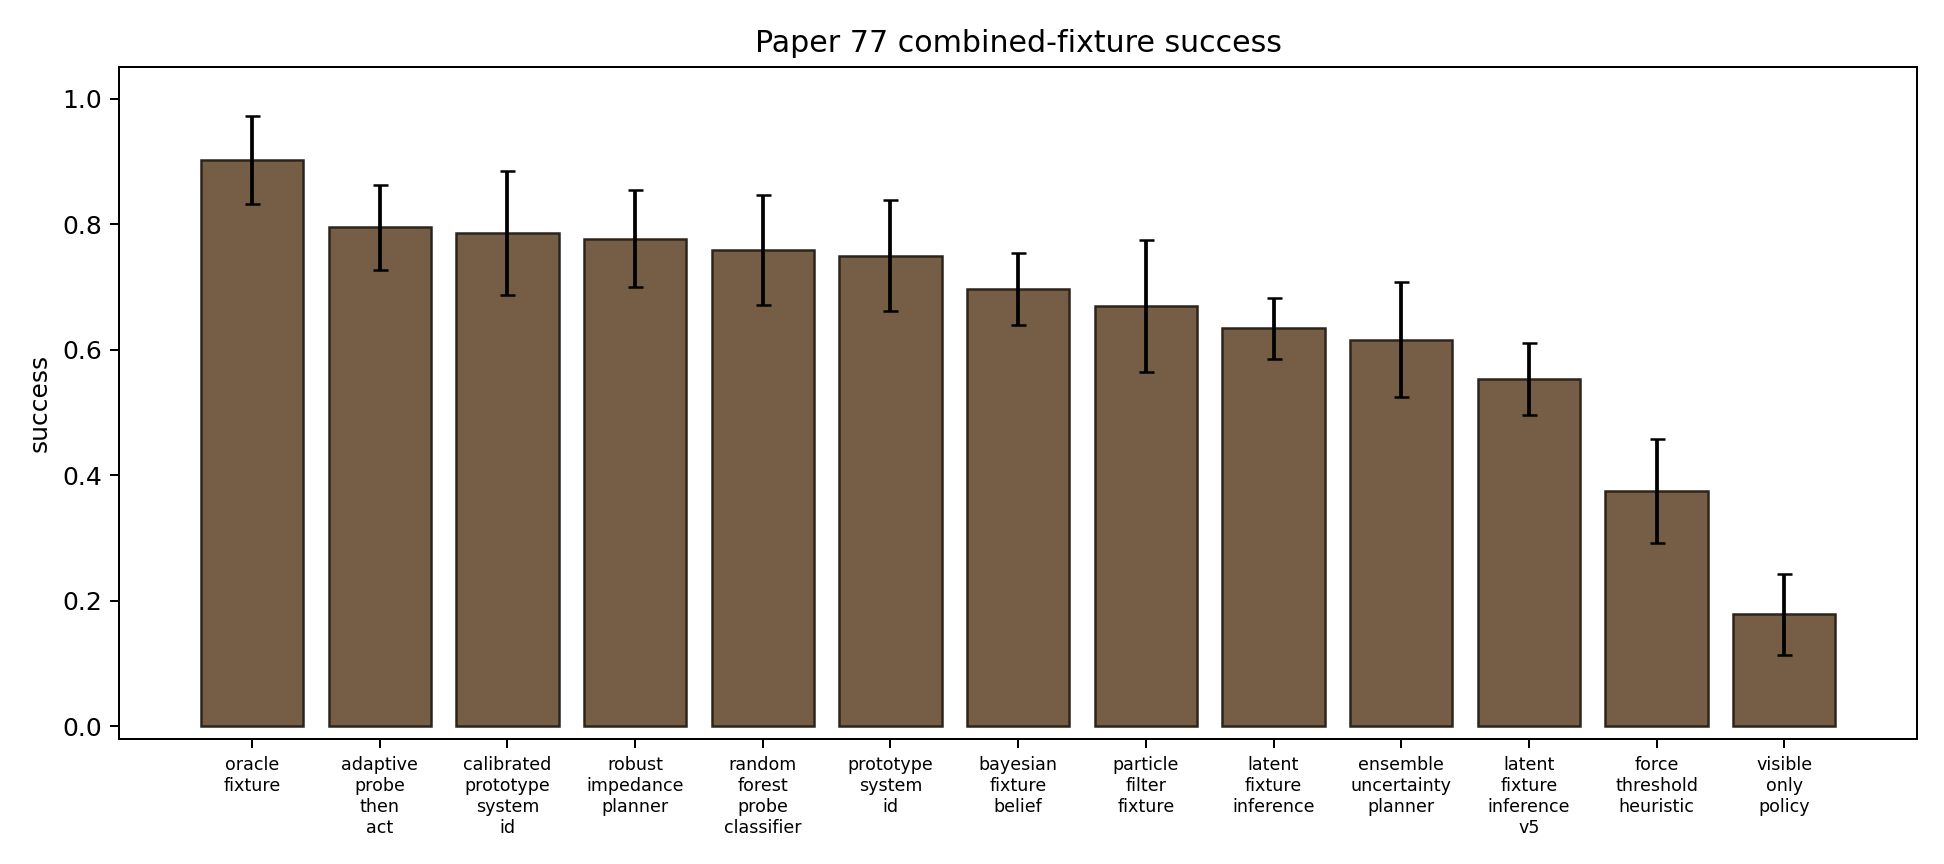
\includegraphics[width=0.92\linewidth]{../figures/latent_fixture_success.png}
\captionof{figure}{Closed-loop success on the decisive combined-fixture-stress split.}
\end{center}
\begin{center}
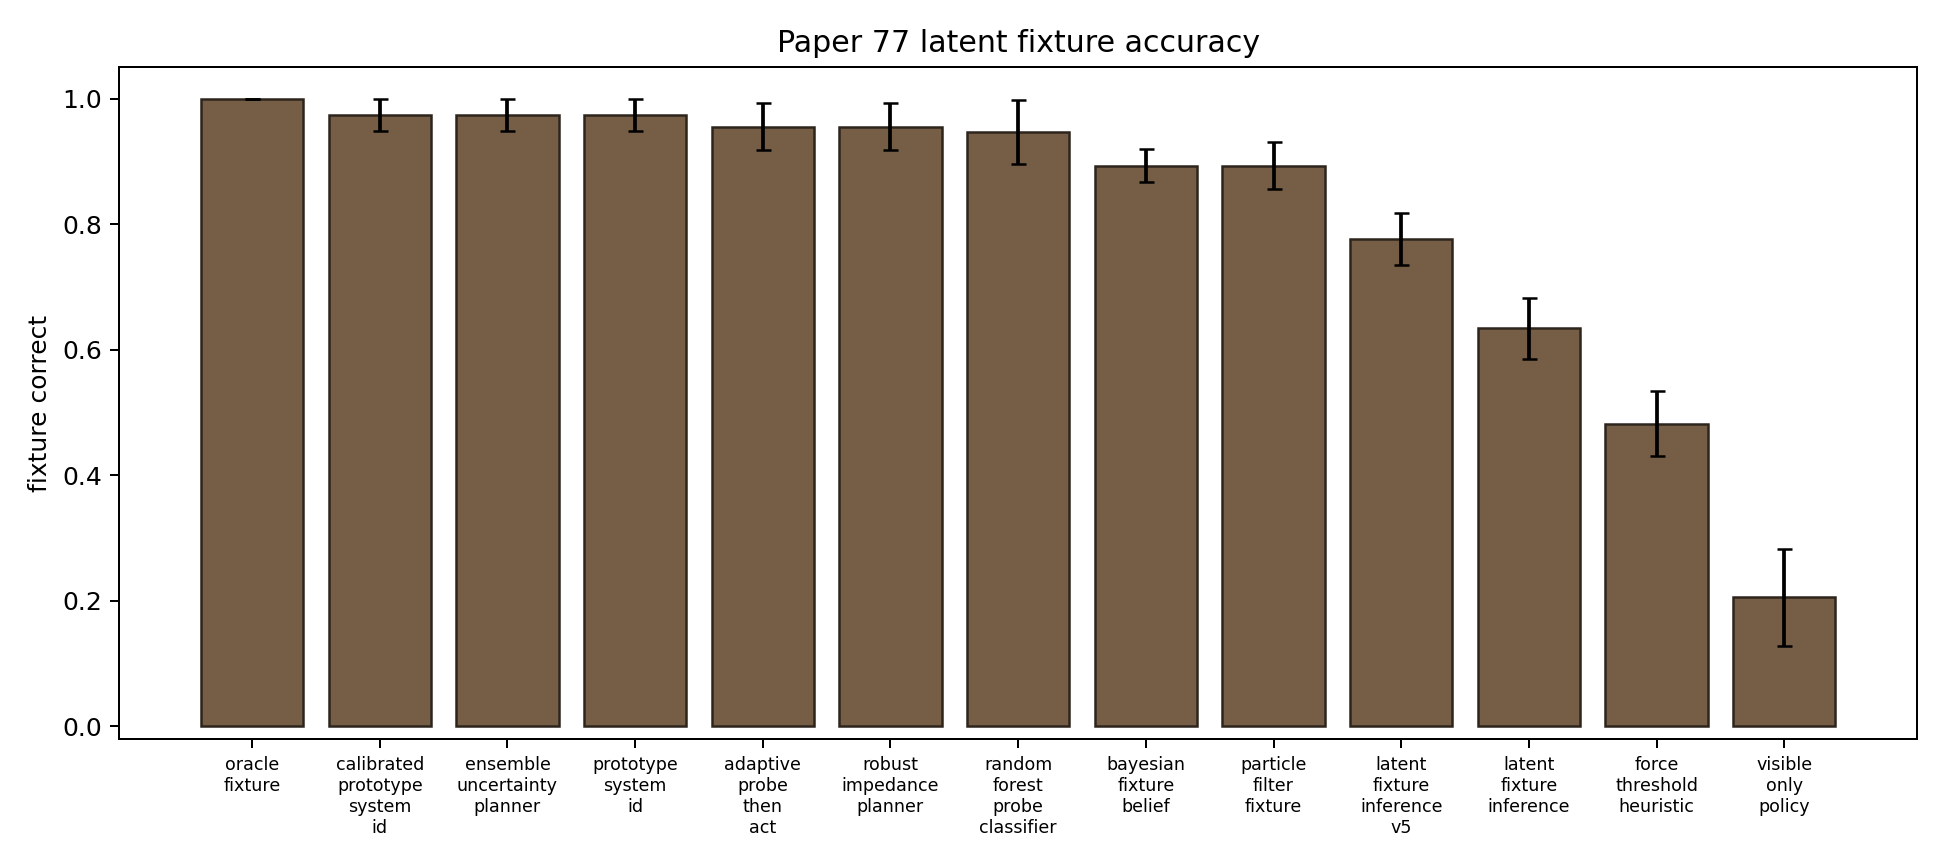
\includegraphics[width=0.92\linewidth]{../figures/latent_fixture_accuracy.png}
\captionof{figure}{Fixture-family accuracy on the decisive split.}
\end{center}

\section{Aggregate Hard Regimes}
\scriptsize
\setlength{\tabcolsep}{2pt}
\begin{center}
\textbf{Table: Aggregate hard-regime metrics}\\[0.4ex]
\resizebox{\linewidth}{!}{%
\begin{tabular}{llccccc}
\toprule
Method & Split & Success & Fixture & Param & Damage & Repeat \\
\midrule
\texttt{oracle} & \texttt{hard-agg} & $0.911 \pm 0.032$ & $1.000 \pm 0.000$ & $0.000 \pm 0.000$ & $0.027 \pm 0.013$ & $0.089 \pm 0.032$ \\
\texttt{adaptive-probe} & \texttt{hard-agg} & $0.859 \pm 0.021$ & $0.987 \pm 0.013$ & $0.209 \pm 0.006$ & $0.029 \pm 0.015$ & $0.141 \pm 0.021$ \\
\texttt{robust-imp} & \texttt{hard-agg} & $0.833 \pm 0.041$ & $0.987 \pm 0.013$ & $0.338 \pm 0.007$ & $0.031 \pm 0.016$ & $0.167 \pm 0.041$ \\
\texttt{rf-probe} & \texttt{hard-agg} & $0.830 \pm 0.025$ & $0.982 \pm 0.016$ & $0.257 \pm 0.009$ & $0.065 \pm 0.017$ & $0.170 \pm 0.025$ \\
\texttt{calib-proto} & \texttt{hard-agg} & $0.821 \pm 0.030$ & $0.991 \pm 0.009$ & $0.205 \pm 0.005$ & $0.047 \pm 0.022$ & $0.179 \pm 0.030$ \\
\texttt{proto-ID} & \texttt{hard-agg} & $0.783 \pm 0.018$ & $0.991 \pm 0.009$ & $0.255 \pm 0.005$ & $0.062 \pm 0.018$ & $0.217 \pm 0.018$ \\
\texttt{bayes} & \texttt{hard-agg} & $0.766 \pm 0.044$ & $0.951 \pm 0.013$ & $0.301 \pm 0.007$ & $0.069 \pm 0.017$ & $0.234 \pm 0.044$ \\
\texttt{particle} & \texttt{hard-agg} & $0.766 \pm 0.042$ & $0.964 \pm 0.013$ & $0.298 \pm 0.007$ & $0.089 \pm 0.026$ & $0.234 \pm 0.042$ \\
\texttt{LFI-v4} & \texttt{hard-agg} & $0.730 \pm 0.023$ & $0.752 \pm 0.015$ & $0.251 \pm 0.009$ & $0.114 \pm 0.019$ & $0.270 \pm 0.023$ \\
\texttt{ensemble} & \texttt{hard-agg} & $0.705 \pm 0.044$ & $0.991 \pm 0.009$ & $0.331 \pm 0.005$ & $0.047 \pm 0.017$ & $0.295 \pm 0.044$ \\
\texttt{LFI-v5} & \texttt{hard-agg} & $0.683 \pm 0.023$ & $0.873 \pm 0.020$ & $0.237 \pm 0.010$ & $0.145 \pm 0.021$ & $0.317 \pm 0.023$ \\
\texttt{threshold} & \texttt{hard-agg} & $0.304 \pm 0.050$ & $0.395 \pm 0.046$ & $0.683 \pm 0.025$ & $0.330 \pm 0.026$ & $0.696 \pm 0.050$ \\
\texttt{visible} & \texttt{hard-agg} & $0.281 \pm 0.043$ & $0.366 \pm 0.029$ & $0.605 \pm 0.019$ & $0.330 \pm 0.040$ & $0.719 \pm 0.043$ \\
\bottomrule
\end{tabular}%
}
\end{center}
\normalsize

The aggregate paired difference against the strongest aggregate baseline is $-0.176\pm 0.039$.  This gate prevents cherry-picking a favorable fixture family.

\scriptsize
\setlength{\tabcolsep}{2pt}
\begin{center}
\textbf{Table: Aggregate paired comparisons}\\[0.4ex]
\resizebox{\linewidth}{!}{%
\begin{tabular}{lcccccc}
\toprule
Comparison & Succ diff & CI & Fixture & Param red & Damage red & Wins \\
\midrule
\texttt{adaptive-probe} & -0.176 & 0.039 & -0.114 & -0.028 & -0.116 & 0/8 \\
\texttt{bayes} & -0.083 & 0.056 & -0.078 & 0.064 & -0.076 & 1/8 \\
\texttt{calib-proto} & -0.138 & 0.037 & -0.118 & -0.032 & -0.098 & 0/8 \\
\texttt{ensemble} & -0.022 & 0.029 & -0.118 & 0.094 & -0.098 & 2/8 \\
\texttt{threshold} & 0.379 & 0.056 & 0.478 & 0.445 & 0.185 & 8/8 \\
\texttt{LFI-v4} & -0.047 & 0.031 & 0.121 & 0.014 & -0.031 & 0/8 \\
\texttt{oracle} & -0.228 & 0.047 & -0.127 & -0.237 & -0.118 & 0/8 \\
\texttt{particle} & -0.083 & 0.035 & -0.092 & 0.061 & -0.056 & 0/8 \\
\texttt{proto-ID} & -0.100 & 0.031 & -0.118 & 0.018 & -0.083 & 0/8 \\
\texttt{rf-probe} & -0.147 & 0.041 & -0.109 & 0.019 & -0.080 & 0/8 \\
\texttt{robust-imp} & -0.150 & 0.058 & -0.114 & 0.101 & -0.114 & 0/8 \\
\texttt{visible} & 0.402 & 0.060 & 0.507 & 0.367 & 0.185 & 8/8 \\
\bottomrule
\end{tabular}%
}
\end{center}
\normalsize

\section{Ablations}
\scriptsize
\setlength{\tabcolsep}{2pt}
\begin{center}
\textbf{Table: LFI-v5 ablations}\\[0.4ex]
\resizebox{\linewidth}{!}{%
\begin{tabular}{lccccc}
\toprule
Variant & Success & Fixture & Param & Damage & Repeat \\
\midrule
\texttt{no-adapt} & $0.700 \pm 0.083$ & $0.812 \pm 0.044$ & $0.266 \pm 0.022$ & $0.050 \pm 0.037$ & $0.300 \pm 0.083$ \\
\texttt{no-calib} & $0.662 \pm 0.104$ & $0.787 \pm 0.044$ & $0.326 \pm 0.022$ & $0.113 \pm 0.094$ & $0.338 \pm 0.104$ \\
\texttt{full-v5} & $0.562 \pm 0.073$ & $0.762 \pm 0.036$ & $0.292 \pm 0.018$ & $0.325 \pm 0.116$ & $0.438 \pm 0.073$ \\
\texttt{no-release} & $0.512 \pm 0.086$ & $0.713 \pm 0.058$ & $0.388 \pm 0.028$ & $0.263 \pm 0.152$ & $0.487 \pm 0.086$ \\
\texttt{no-margin} & $0.500 \pm 0.091$ & $0.762 \pm 0.036$ & $0.292 \pm 0.018$ & $0.375 \pm 0.081$ & $0.500 \pm 0.091$ \\
\texttt{no-hysteresis} & $0.487 \pm 0.086$ & $0.600 \pm 0.037$ & $0.439 \pm 0.018$ & $0.263 \pm 0.104$ & $0.512 \pm 0.086$ \\
\texttt{no-aniso} & $0.438 \pm 0.073$ & $0.688 \pm 0.058$ & $0.399 \pm 0.028$ & $0.250 \pm 0.083$ & $0.562 \pm 0.073$ \\
\texttt{no-particle} & $0.350 \pm 0.064$ & $0.375 \pm 0.072$ & $0.479 \pm 0.035$ & $0.225 \pm 0.103$ & $0.650 \pm 0.064$ \\
\texttt{no-torque} & $0.300 \pm 0.074$ & $0.400 \pm 0.098$ & $0.539 \pm 0.047$ & $0.375 \pm 0.096$ & $0.700 \pm 0.074$ \\
\bottomrule
\end{tabular}%
}
\end{center}
\normalsize

\begin{center}
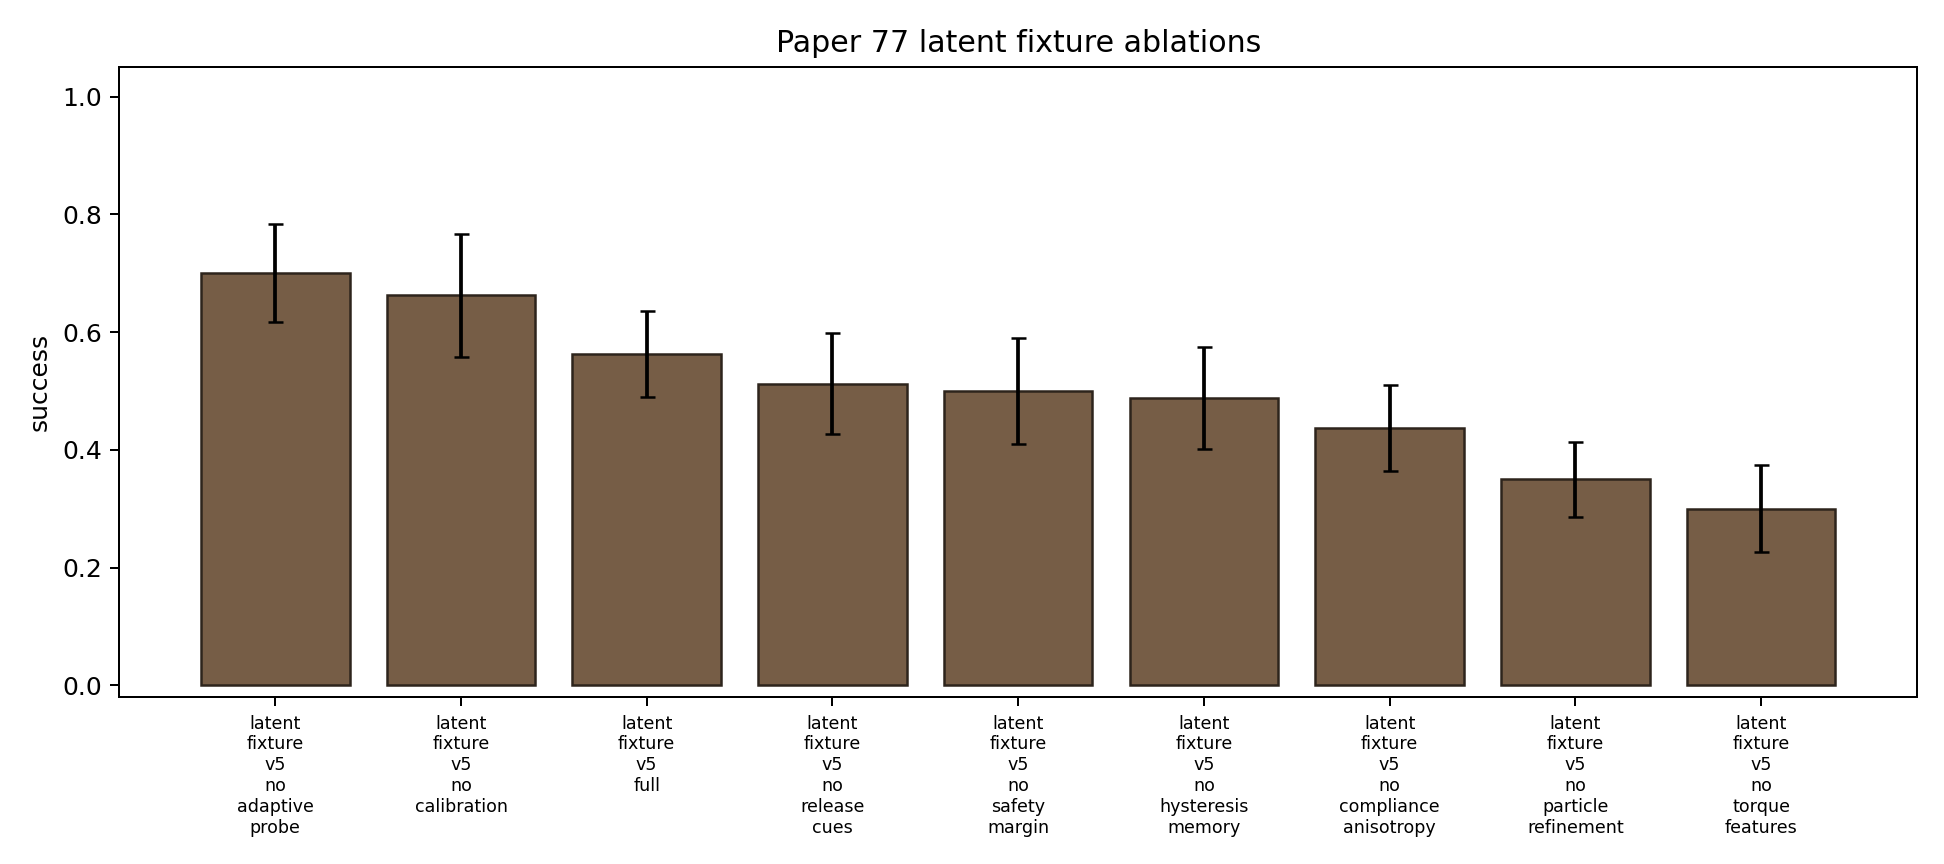
\includegraphics[width=0.92\linewidth]{../figures/latent_fixture_ablation_success.png}
\captionof{figure}{Ablation success. Full v5 must beat component removals to support the mechanism.}
\end{center}

\section{Stress Sweep}
\scriptsize
\setlength{\tabcolsep}{2pt}
\begin{center}
\textbf{Table: Stress sweep}\\[0.4ex]
\resizebox{\linewidth}{!}{%
\begin{tabular}{llcccc}
\toprule
Method & Stress & Success & Fixture & Damage & Repeat \\
\midrule
\texttt{adaptive-probe} & 0.00 & $0.828 \pm 0.079$ & $0.953 \pm 0.045$ & $0.078 \pm 0.064$ & $0.172 \pm 0.079$ \\
\texttt{bayes} & 0.00 & $0.719 \pm 0.090$ & $0.906 \pm 0.061$ & $0.172 \pm 0.064$ & $0.281 \pm 0.090$ \\
\texttt{calib-proto} & 0.00 & $0.797 \pm 0.122$ & $0.969 \pm 0.040$ & $0.047 \pm 0.045$ & $0.203 \pm 0.122$ \\
\texttt{ensemble} & 0.00 & $0.609 \pm 0.108$ & $0.969 \pm 0.040$ & $0.141 \pm 0.086$ & $0.391 \pm 0.108$ \\
\texttt{LFI-v5} & 0.00 & $0.594 \pm 0.090$ & $0.781 \pm 0.077$ & $0.312 \pm 0.080$ & $0.406 \pm 0.090$ \\
\texttt{oracle} & 0.00 & $0.844 \pm 0.111$ & $1.000 \pm 0.000$ & $0.031 \pm 0.040$ & $0.156 \pm 0.111$ \\
\texttt{particle} & 0.00 & $0.734 \pm 0.108$ & $0.906 \pm 0.040$ & $0.125 \pm 0.000$ & $0.266 \pm 0.108$ \\
\texttt{proto-ID} & 0.00 & $0.656 \pm 0.159$ & $0.969 \pm 0.040$ & $0.062 \pm 0.065$ & $0.344 \pm 0.159$ \\
\texttt{rf-probe} & 0.00 & $0.781 \pm 0.152$ & $0.969 \pm 0.040$ & $0.062 \pm 0.065$ & $0.219 \pm 0.152$ \\
\texttt{robust-imp} & 0.00 & $0.734 \pm 0.086$ & $0.969 \pm 0.040$ & $0.203 \pm 0.122$ & $0.266 \pm 0.086$ \\
\texttt{adaptive-probe} & 0.20 & $0.844 \pm 0.120$ & $0.953 \pm 0.045$ & $0.062 \pm 0.065$ & $0.156 \pm 0.120$ \\
\texttt{bayes} & 0.20 & $0.641 \pm 0.086$ & $0.828 \pm 0.045$ & $0.172 \pm 0.064$ & $0.359 \pm 0.086$ \\
\texttt{calib-proto} & 0.20 & $0.859 \pm 0.056$ & $0.969 \pm 0.040$ & $0.047 \pm 0.045$ & $0.141 \pm 0.056$ \\
\texttt{ensemble} & 0.20 & $0.547 \pm 0.153$ & $0.969 \pm 0.040$ & $0.172 \pm 0.103$ & $0.453 \pm 0.153$ \\
\texttt{LFI-v5} & 0.20 & $0.547 \pm 0.045$ & $0.734 \pm 0.086$ & $0.344 \pm 0.120$ & $0.453 \pm 0.045$ \\
\texttt{oracle} & 0.20 & $0.844 \pm 0.111$ & $1.000 \pm 0.000$ & $0.000 \pm 0.000$ & $0.156 \pm 0.111$ \\
\texttt{particle} & 0.20 & $0.656 \pm 0.101$ & $0.859 \pm 0.031$ & $0.125 \pm 0.093$ & $0.344 \pm 0.101$ \\
\texttt{proto-ID} & 0.20 & $0.734 \pm 0.117$ & $0.969 \pm 0.040$ & $0.062 \pm 0.046$ & $0.266 \pm 0.117$ \\
\texttt{rf-probe} & 0.20 & $0.797 \pm 0.079$ & $0.938 \pm 0.065$ & $0.078 \pm 0.064$ & $0.203 \pm 0.079$ \\
\texttt{robust-imp} & 0.20 & $0.672 \pm 0.045$ & $0.953 \pm 0.045$ & $0.156 \pm 0.101$ & $0.328 \pm 0.045$ \\
\texttt{adaptive-probe} & 0.40 & $0.750 \pm 0.122$ & $0.891 \pm 0.056$ & $0.078 \pm 0.045$ & $0.250 \pm 0.122$ \\
\texttt{bayes} & 0.40 & $0.578 \pm 0.122$ & $0.828 \pm 0.079$ & $0.125 \pm 0.080$ & $0.422 \pm 0.122$ \\
\texttt{calib-proto} & 0.40 & $0.672 \pm 0.113$ & $0.938 \pm 0.065$ & $0.094 \pm 0.077$ & $0.328 \pm 0.113$ \\
\texttt{ensemble} & 0.40 & $0.469 \pm 0.145$ & $0.938 \pm 0.065$ & $0.219 \pm 0.061$ & $0.531 \pm 0.145$ \\
\texttt{LFI-v5} & 0.40 & $0.406 \pm 0.101$ & $0.672 \pm 0.045$ & $0.406 \pm 0.090$ & $0.594 \pm 0.101$ \\
\texttt{oracle} & 0.40 & $0.828 \pm 0.064$ & $1.000 \pm 0.000$ & $0.031 \pm 0.061$ & $0.172 \pm 0.064$ \\
\texttt{particle} & 0.40 & $0.656 \pm 0.101$ & $0.891 \pm 0.056$ & $0.109 \pm 0.072$ & $0.344 \pm 0.101$ \\
\texttt{proto-ID} & 0.40 & $0.719 \pm 0.090$ & $0.938 \pm 0.065$ & $0.234 \pm 0.126$ & $0.281 \pm 0.090$ \\
\texttt{rf-probe} & 0.40 & $0.641 \pm 0.108$ & $0.875 \pm 0.065$ & $0.172 \pm 0.064$ & $0.359 \pm 0.108$ \\
\texttt{robust-imp} & 0.40 & $0.625 \pm 0.104$ & $0.906 \pm 0.061$ & $0.203 \pm 0.079$ & $0.375 \pm 0.104$ \\
\texttt{adaptive-probe} & 0.60 & $0.672 \pm 0.130$ & $0.969 \pm 0.040$ & $0.125 \pm 0.065$ & $0.328 \pm 0.130$ \\
\texttt{bayes} & 0.60 & $0.547 \pm 0.092$ & $0.844 \pm 0.077$ & $0.250 \pm 0.104$ & $0.453 \pm 0.092$ \\
\texttt{calib-proto} & 0.60 & $0.703 \pm 0.138$ & $0.953 \pm 0.045$ & $0.125 \pm 0.065$ & $0.297 \pm 0.138$ \\
\texttt{ensemble} & 0.60 & $0.547 \pm 0.113$ & $0.953 \pm 0.045$ & $0.266 \pm 0.072$ & $0.453 \pm 0.113$ \\
\bottomrule
\end{tabular}%
}
\end{center}
\begin{center}
\textbf{Table: Stress sweep continued}\\[0.4ex]
\resizebox{\linewidth}{!}{%
\begin{tabular}{llcccc}
\toprule
Method & Stress & Success & Fixture & Damage & Repeat \\
\midrule
\texttt{LFI-v5} & 0.60 & $0.359 \pm 0.086$ & $0.672 \pm 0.113$ & $0.406 \pm 0.090$ & $0.641 \pm 0.086$ \\
\texttt{oracle} & 0.60 & $0.859 \pm 0.098$ & $1.000 \pm 0.000$ & $0.016 \pm 0.031$ & $0.141 \pm 0.098$ \\
\texttt{particle} & 0.60 & $0.500 \pm 0.093$ & $0.812 \pm 0.080$ & $0.125 \pm 0.080$ & $0.500 \pm 0.093$ \\
\texttt{proto-ID} & 0.60 & $0.609 \pm 0.117$ & $0.938 \pm 0.046$ & $0.203 \pm 0.103$ & $0.391 \pm 0.117$ \\
\texttt{rf-probe} & 0.60 & $0.609 \pm 0.108$ & $0.906 \pm 0.040$ & $0.125 \pm 0.065$ & $0.391 \pm 0.108$ \\
\texttt{robust-imp} & 0.60 & $0.672 \pm 0.113$ & $0.969 \pm 0.040$ & $0.344 \pm 0.101$ & $0.328 \pm 0.113$ \\
\texttt{adaptive-probe} & 0.80 & $0.734 \pm 0.098$ & $0.922 \pm 0.064$ & $0.062 \pm 0.046$ & $0.266 \pm 0.098$ \\
\texttt{bayes} & 0.80 & $0.641 \pm 0.214$ & $0.844 \pm 0.090$ & $0.250 \pm 0.104$ & $0.359 \pm 0.214$ \\
\texttt{calib-proto} & 0.80 & $0.656 \pm 0.159$ & $0.875 \pm 0.065$ & $0.203 \pm 0.079$ & $0.344 \pm 0.159$ \\
\texttt{ensemble} & 0.80 & $0.453 \pm 0.103$ & $0.875 \pm 0.065$ & $0.250 \pm 0.131$ & $0.547 \pm 0.103$ \\
\texttt{LFI-v5} & 0.80 & $0.484 \pm 0.117$ & $0.750 \pm 0.093$ & $0.375 \pm 0.065$ & $0.516 \pm 0.117$ \\
\texttt{oracle} & 0.80 & $0.875 \pm 0.065$ & $1.000 \pm 0.000$ & $0.031 \pm 0.040$ & $0.125 \pm 0.065$ \\
\texttt{particle} & 0.80 & $0.562 \pm 0.113$ & $0.859 \pm 0.056$ & $0.281 \pm 0.120$ & $0.438 \pm 0.113$ \\
\texttt{proto-ID} & 0.80 & $0.656 \pm 0.090$ & $0.875 \pm 0.065$ & $0.234 \pm 0.134$ & $0.344 \pm 0.090$ \\
\texttt{rf-probe} & 0.80 & $0.734 \pm 0.126$ & $0.938 \pm 0.065$ & $0.188 \pm 0.065$ & $0.266 \pm 0.126$ \\
\texttt{robust-imp} & 0.80 & $0.469 \pm 0.101$ & $0.875 \pm 0.080$ & $0.297 \pm 0.113$ & $0.531 \pm 0.101$ \\
\texttt{adaptive-probe} & 1.00 & $0.656 \pm 0.077$ & $0.859 \pm 0.056$ & $0.219 \pm 0.120$ & $0.344 \pm 0.077$ \\
\texttt{bayes} & 1.00 & $0.500 \pm 0.113$ & $0.797 \pm 0.122$ & $0.234 \pm 0.117$ & $0.500 \pm 0.113$ \\
\texttt{calib-proto} & 1.00 & $0.594 \pm 0.090$ & $0.844 \pm 0.111$ & $0.203 \pm 0.122$ & $0.406 \pm 0.090$ \\
\texttt{ensemble} & 1.00 & $0.375 \pm 0.080$ & $0.859 \pm 0.098$ & $0.359 \pm 0.134$ & $0.625 \pm 0.080$ \\
\texttt{LFI-v5} & 1.00 & $0.344 \pm 0.090$ & $0.609 \pm 0.098$ & $0.438 \pm 0.122$ & $0.656 \pm 0.090$ \\
\texttt{oracle} & 1.00 & $0.812 \pm 0.065$ & $1.000 \pm 0.000$ & $0.031 \pm 0.040$ & $0.188 \pm 0.065$ \\
\texttt{particle} & 1.00 & $0.609 \pm 0.126$ & $0.844 \pm 0.090$ & $0.156 \pm 0.137$ & $0.391 \pm 0.126$ \\
\texttt{proto-ID} & 1.00 & $0.641 \pm 0.142$ & $0.859 \pm 0.098$ & $0.188 \pm 0.113$ & $0.359 \pm 0.142$ \\
\texttt{rf-probe} & 1.00 & $0.625 \pm 0.154$ & $0.859 \pm 0.072$ & $0.188 \pm 0.065$ & $0.375 \pm 0.154$ \\
\texttt{robust-imp} & 1.00 & $0.516 \pm 0.108$ & $0.859 \pm 0.098$ & $0.312 \pm 0.080$ & $0.484 \pm 0.108$ \\
\texttt{adaptive-probe} & 1.20 & $0.594 \pm 0.172$ & $0.812 \pm 0.104$ & $0.203 \pm 0.092$ & $0.406 \pm 0.172$ \\
\texttt{bayes} & 1.20 & $0.453 \pm 0.146$ & $0.750 \pm 0.046$ & $0.344 \pm 0.090$ & $0.547 \pm 0.146$ \\
\texttt{calib-proto} & 1.20 & $0.641 \pm 0.117$ & $0.844 \pm 0.101$ & $0.172 \pm 0.103$ & $0.359 \pm 0.117$ \\
\texttt{ensemble} & 1.20 & $0.453 \pm 0.113$ & $0.844 \pm 0.090$ & $0.312 \pm 0.065$ & $0.547 \pm 0.113$ \\
\texttt{LFI-v5} & 1.20 & $0.406 \pm 0.120$ & $0.547 \pm 0.092$ & $0.531 \pm 0.152$ & $0.594 \pm 0.120$ \\
\texttt{oracle} & 1.20 & $0.828 \pm 0.064$ & $1.000 \pm 0.000$ & $0.047 \pm 0.064$ & $0.172 \pm 0.064$ \\
\texttt{particle} & 1.20 & $0.562 \pm 0.104$ & $0.797 \pm 0.045$ & $0.203 \pm 0.103$ & $0.438 \pm 0.104$ \\
\texttt{proto-ID} & 1.20 & $0.578 \pm 0.179$ & $0.844 \pm 0.101$ & $0.219 \pm 0.061$ & $0.422 \pm 0.179$ \\
\bottomrule
\end{tabular}%
}
\end{center}
\begin{center}
\textbf{Table: Stress sweep continued}\\[0.4ex]
\resizebox{\linewidth}{!}{%
\begin{tabular}{llcccc}
\toprule
Method & Stress & Success & Fixture & Damage & Repeat \\
\midrule
\texttt{rf-probe} & 1.20 & $0.609 \pm 0.108$ & $0.766 \pm 0.108$ & $0.281 \pm 0.111$ & $0.391 \pm 0.108$ \\
\texttt{robust-imp} & 1.20 & $0.438 \pm 0.104$ & $0.844 \pm 0.101$ & $0.219 \pm 0.111$ & $0.562 \pm 0.104$ \\
\bottomrule
\end{tabular}%
}
\end{center}
\normalsize

At maximum stress 1.20, LFI-v5 reaches $0.406 \pm 0.120$ success while the strongest non-oracle stress baseline reaches $0.641 \pm 0.117$.  This gate is reported even when unfavorable.

\begin{center}
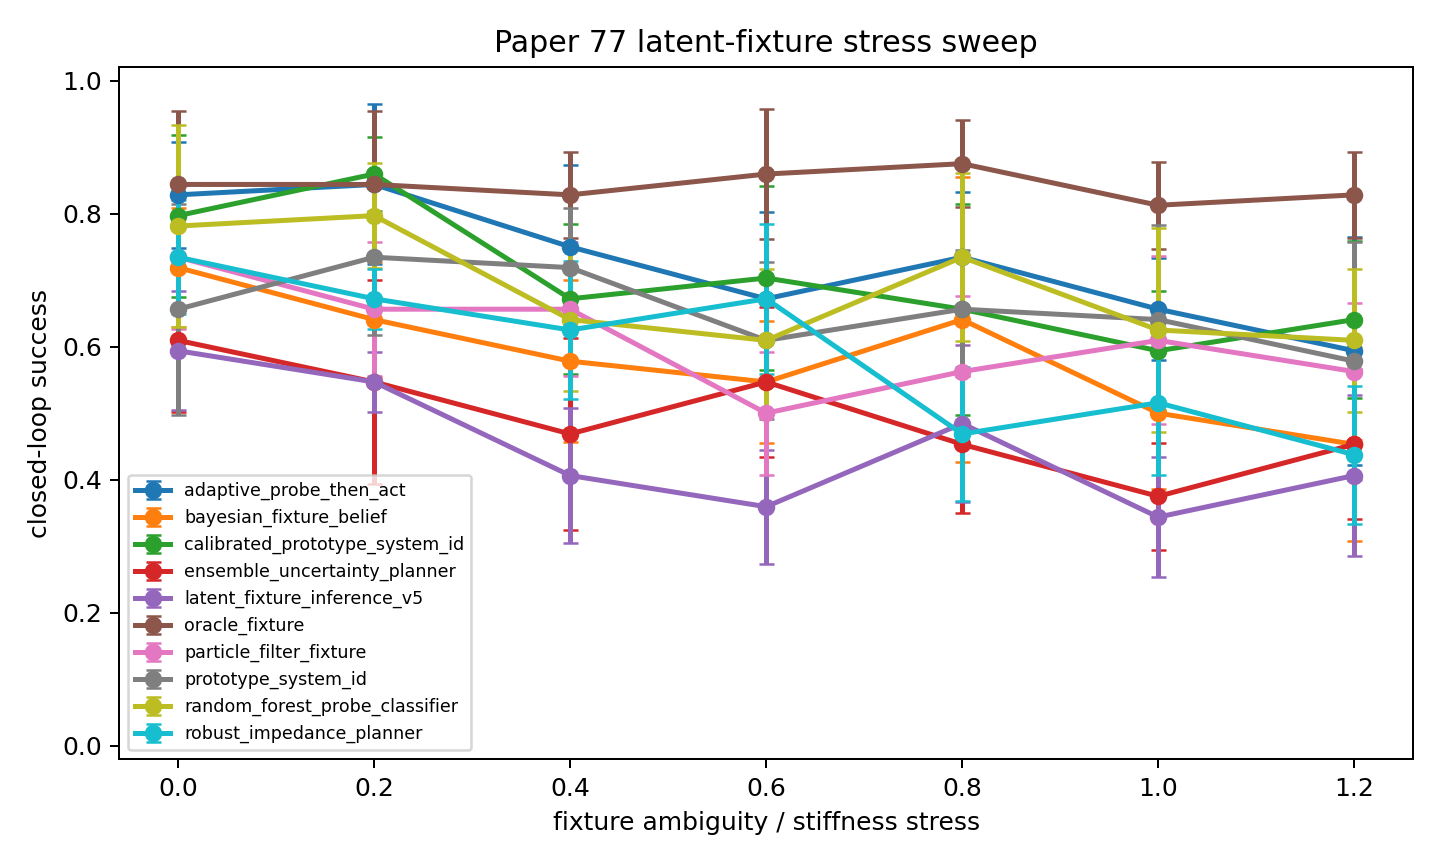
\includegraphics[width=0.92\linewidth]{../figures/latent_fixture_stress_sweep.png}
\captionof{figure}{Success under increasing fixture ambiguity, stiffness shift, noise, and slip.}
\end{center}

\section{Fixed-Risk Budgets}
\scriptsize
\setlength{\tabcolsep}{2pt}
\begin{center}
\textbf{Table: Fixed-risk budget metrics}\\[0.4ex]
\resizebox{\linewidth}{!}{%
\begin{tabular}{llccccc}
\toprule
Method & Budget & Success & Fixture & Damage & Repeat & Efficiency \\
\midrule
\texttt{adaptive-probe} & 0.08 & $0.703 \pm 0.079$ & $0.953 \pm 0.045$ & $0.078 \pm 0.045$ & $0.266 \pm 0.098$ & $0.566 \pm 0.054$ \\
\texttt{rf-probe} & 0.08 & $0.578 \pm 0.092$ & $0.938 \pm 0.065$ & $0.188 \pm 0.065$ & $0.281 \pm 0.152$ & $0.506 \pm 0.074$ \\
\texttt{proto-ID} & 0.08 & $0.562 \pm 0.093$ & $0.953 \pm 0.045$ & $0.172 \pm 0.079$ & $0.219 \pm 0.061$ & $0.519 \pm 0.055$ \\
\texttt{calib-proto} & 0.08 & $0.531 \pm 0.129$ & $0.953 \pm 0.045$ & $0.141 \pm 0.098$ & $0.266 \pm 0.098$ & $0.496 \pm 0.069$ \\
\texttt{particle} & 0.08 & $0.516 \pm 0.126$ & $0.859 \pm 0.086$ & $0.172 \pm 0.079$ & $0.344 \pm 0.077$ & $0.458 \pm 0.067$ \\
\texttt{bayes} & 0.08 & $0.453 \pm 0.130$ & $0.844 \pm 0.061$ & $0.188 \pm 0.093$ & $0.422 \pm 0.153$ & $0.410 \pm 0.091$ \\
\texttt{robust-imp} & 0.08 & $0.438 \pm 0.122$ & $0.938 \pm 0.046$ & $0.297 \pm 0.113$ & $0.438 \pm 0.093$ & $0.390 \pm 0.073$ \\
\texttt{LFI-v5} & 0.08 & $0.266 \pm 0.086$ & $0.719 \pm 0.061$ & $0.359 \pm 0.108$ & $0.516 \pm 0.150$ & $0.265 \pm 0.074$ \\
\texttt{adaptive-probe} & 0.12 & $0.719 \pm 0.159$ & $0.953 \pm 0.045$ & $0.062 \pm 0.046$ & $0.281 \pm 0.159$ & $0.572 \pm 0.105$ \\
\texttt{calib-proto} & 0.12 & $0.609 \pm 0.098$ & $0.953 \pm 0.045$ & $0.094 \pm 0.061$ & $0.234 \pm 0.056$ & $0.538 \pm 0.052$ \\
\texttt{particle} & 0.12 & $0.594 \pm 0.077$ & $0.875 \pm 0.065$ & $0.203 \pm 0.079$ & $0.312 \pm 0.065$ & $0.497 \pm 0.043$ \\
\texttt{rf-probe} & 0.12 & $0.547 \pm 0.160$ & $0.953 \pm 0.064$ & $0.125 \pm 0.080$ & $0.344 \pm 0.178$ & $0.487 \pm 0.111$ \\
\texttt{proto-ID} & 0.12 & $0.500 \pm 0.122$ & $0.953 \pm 0.045$ & $0.172 \pm 0.045$ & $0.312 \pm 0.173$ & $0.473 \pm 0.088$ \\
\texttt{bayes} & 0.12 & $0.438 \pm 0.113$ & $0.875 \pm 0.046$ & $0.203 \pm 0.079$ & $0.438 \pm 0.113$ & $0.403 \pm 0.071$ \\
\texttt{robust-imp} & 0.12 & $0.422 \pm 0.092$ & $0.938 \pm 0.046$ & $0.250 \pm 0.122$ & $0.422 \pm 0.064$ & $0.384 \pm 0.047$ \\
\texttt{LFI-v5} & 0.12 & $0.266 \pm 0.072$ & $0.734 \pm 0.031$ & $0.281 \pm 0.090$ & $0.547 \pm 0.113$ & $0.263 \pm 0.055$ \\
\texttt{calib-proto} & 0.18 & $0.641 \pm 0.134$ & $0.922 \pm 0.045$ & $0.047 \pm 0.045$ & $0.281 \pm 0.111$ & $0.534 \pm 0.085$ \\
\texttt{adaptive-probe} & 0.18 & $0.625 \pm 0.154$ & $0.922 \pm 0.045$ & $0.125 \pm 0.093$ & $0.328 \pm 0.138$ & $0.516 \pm 0.099$ \\
\texttt{particle} & 0.18 & $0.531 \pm 0.077$ & $0.875 \pm 0.046$ & $0.234 \pm 0.086$ & $0.266 \pm 0.086$ & $0.483 \pm 0.044$ \\
\texttt{proto-ID} & 0.18 & $0.500 \pm 0.131$ & $0.906 \pm 0.040$ & $0.141 \pm 0.086$ & $0.375 \pm 0.122$ & $0.453 \pm 0.074$ \\
\texttt{rf-probe} & 0.18 & $0.500 \pm 0.122$ & $0.891 \pm 0.056$ & $0.141 \pm 0.086$ & $0.375 \pm 0.093$ & $0.453 \pm 0.071$ \\
\texttt{bayes} & 0.18 & $0.484 \pm 0.098$ & $0.828 \pm 0.064$ & $0.203 \pm 0.113$ & $0.422 \pm 0.079$ & $0.422 \pm 0.048$ \\
\texttt{robust-imp} & 0.18 & $0.453 \pm 0.103$ & $0.938 \pm 0.046$ & $0.234 \pm 0.086$ & $0.406 \pm 0.090$ & $0.402 \pm 0.064$ \\
\texttt{LFI-v5} & 0.18 & $0.266 \pm 0.072$ & $0.703 \pm 0.092$ & $0.344 \pm 0.145$ & $0.547 \pm 0.122$ & $0.260 \pm 0.062$ \\
\texttt{adaptive-probe} & 0.25 & $0.672 \pm 0.064$ & $0.969 \pm 0.040$ & $0.062 \pm 0.046$ & $0.250 \pm 0.080$ & $0.562 \pm 0.037$ \\
\texttt{proto-ID} & 0.25 & $0.594 \pm 0.137$ & $0.969 \pm 0.040$ & $0.062 \pm 0.065$ & $0.328 \pm 0.153$ & $0.511 \pm 0.091$ \\
\texttt{calib-proto} & 0.25 & $0.562 \pm 0.139$ & $0.969 \pm 0.040$ & $0.172 \pm 0.113$ & $0.234 \pm 0.134$ & $0.516 \pm 0.090$ \\
\texttt{bayes} & 0.25 & $0.547 \pm 0.103$ & $0.859 \pm 0.056$ & $0.141 \pm 0.056$ & $0.375 \pm 0.104$ & $0.461 \pm 0.060$ \\
\texttt{rf-probe} & 0.25 & $0.516 \pm 0.126$ & $0.906 \pm 0.090$ & $0.125 \pm 0.122$ & $0.359 \pm 0.150$ & $0.464 \pm 0.092$ \\
\texttt{particle} & 0.25 & $0.484 \pm 0.098$ & $0.859 \pm 0.086$ & $0.172 \pm 0.113$ & $0.422 \pm 0.079$ & $0.431 \pm 0.065$ \\
\texttt{robust-imp} & 0.25 & $0.484 \pm 0.142$ & $0.969 \pm 0.040$ & $0.250 \pm 0.139$ & $0.344 \pm 0.137$ & $0.432 \pm 0.095$ \\
\texttt{LFI-v5} & 0.25 & $0.172 \pm 0.064$ & $0.703 \pm 0.092$ & $0.422 \pm 0.153$ & $0.578 \pm 0.092$ & $0.209 \pm 0.041$ \\
\bottomrule
\end{tabular}%
}
\end{center}
\normalsize

\scriptsize
\setlength{\tabcolsep}{2pt}
\begin{center}
\textbf{Table: Fixed-risk paired comparisons}\\[0.4ex]
\resizebox{\linewidth}{!}{%
\begin{tabular}{llccccc}
\toprule
Budget & Comparison & Succ diff & CI & Fixture & Damage & Wins \\
\midrule
0.08 & \texttt{adaptive-probe} & -0.438 & 0.154 & -0.234 & -0.281 & 0/8 \\
0.08 & \texttt{bayes} & -0.188 & 0.104 & -0.125 & -0.172 & 0/8 \\
0.08 & \texttt{calib-proto} & -0.266 & 0.117 & -0.234 & -0.219 & 0/8 \\
0.08 & \texttt{particle} & -0.250 & 0.122 & -0.141 & -0.188 & 0/8 \\
0.08 & \texttt{proto-ID} & -0.297 & 0.079 & -0.234 & -0.188 & 0/8 \\
0.08 & \texttt{rf-probe} & -0.312 & 0.113 & -0.219 & -0.172 & 0/8 \\
0.08 & \texttt{robust-imp} & -0.172 & 0.103 & -0.219 & -0.062 & 0/8 \\
0.12 & \texttt{adaptive-probe} & -0.453 & 0.173 & -0.219 & -0.219 & 0/8 \\
0.12 & \texttt{bayes} & -0.172 & 0.160 & -0.141 & -0.078 & 1/8 \\
0.12 & \texttt{calib-proto} & -0.344 & 0.077 & -0.219 & -0.188 & 0/8 \\
0.12 & \texttt{particle} & -0.328 & 0.064 & -0.141 & -0.078 & 0/8 \\
0.12 & \texttt{proto-ID} & -0.234 & 0.117 & -0.219 & -0.109 & 0/8 \\
0.12 & \texttt{rf-probe} & -0.281 & 0.189 & -0.219 & -0.156 & 1/8 \\
0.12 & \texttt{robust-imp} & -0.156 & 0.137 & -0.203 & -0.031 & 1/8 \\
0.18 & \texttt{adaptive-probe} & -0.359 & 0.117 & -0.219 & -0.219 & 0/8 \\
0.18 & \texttt{bayes} & -0.219 & 0.111 & -0.125 & -0.141 & 0/8 \\
0.18 & \texttt{calib-proto} & -0.375 & 0.146 & -0.219 & -0.297 & 0/8 \\
0.18 & \texttt{particle} & -0.266 & 0.098 & -0.172 & -0.109 & 0/8 \\
0.18 & \texttt{proto-ID} & -0.234 & 0.126 & -0.203 & -0.203 & 0/8 \\
0.18 & \texttt{rf-probe} & -0.234 & 0.142 & -0.188 & -0.203 & 0/8 \\
0.18 & \texttt{robust-imp} & -0.188 & 0.139 & -0.234 & -0.109 & 1/8 \\
0.25 & \texttt{adaptive-probe} & -0.500 & 0.080 & -0.266 & -0.359 & 0/8 \\
0.25 & \texttt{bayes} & -0.375 & 0.139 & -0.156 & -0.281 & 0/8 \\
0.25 & \texttt{calib-proto} & -0.391 & 0.170 & -0.266 & -0.250 & 0/8 \\
0.25 & \texttt{particle} & -0.312 & 0.104 & -0.156 & -0.250 & 0/8 \\
0.25 & \texttt{proto-ID} & -0.422 & 0.153 & -0.266 & -0.359 & 0/8 \\
0.25 & \texttt{rf-probe} & -0.344 & 0.129 & -0.203 & -0.297 & 0/8 \\
0.25 & \texttt{robust-imp} & -0.312 & 0.139 & -0.266 & -0.172 & 0/8 \\
\bottomrule
\end{tabular}%
}
\end{center}
\normalsize

\begin{center}
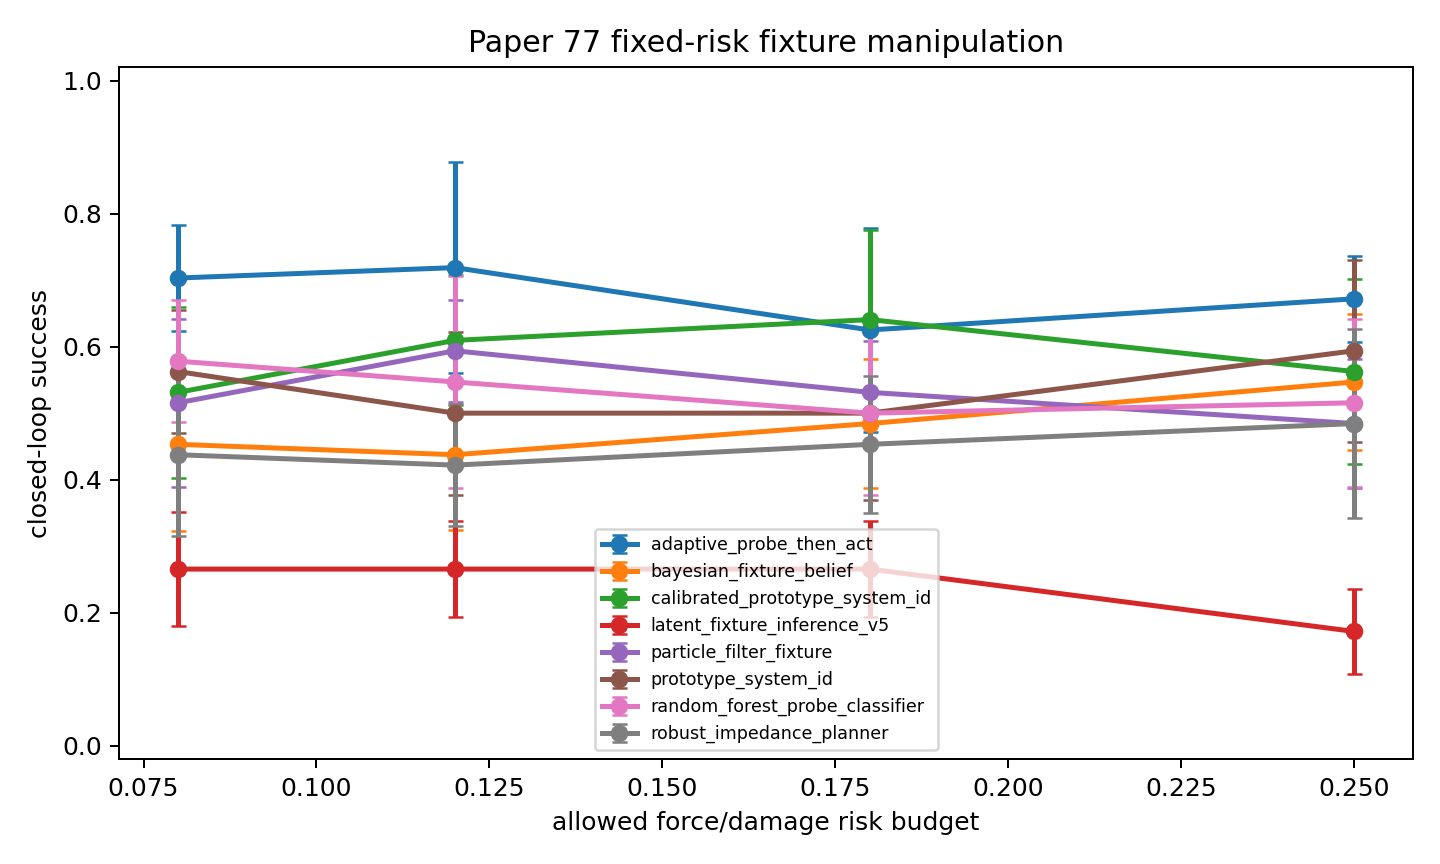
\includegraphics[width=0.92\linewidth]{../figures/latent_fixture_fixed_risk.png}
\captionof{figure}{Fixed-risk success across predefined force/damage budgets.}
\end{center}

\section{Negative Cases}
\scriptsize
\setlength{\tabcolsep}{2pt}
\begin{center}
\textbf{Table: Curated combined-stress negative cases}\\[0.4ex]
\resizebox{\linewidth}{!}{%
\begin{tabular}{llllllll}
\toprule
Seed & Scenario & True & Estimate & Action & Force & Damage & Param \\
\midrule
0 & 4001 & tether & tether & cautious\_probe\_pull & 1 & 0 & 0.186 \\
0 & 4003 & clamp & suction & cautious\_probe\_pull & 1 & 0 & 0.660 \\
0 & 4004 & hinge & hinge & pivot\_rotate & 0 & 0 & 0.176 \\
0 & 4005 & slot & slot & cautious\_probe\_pull & 1 & 0 & 0.185 \\
0 & 4007 & tether & tether & cautious\_probe\_pull & 0 & 0 & 0.183 \\
0 & 4009 & clamp & suction & peel\_then\_translate & 0 & 0 & 0.660 \\
0 & 4013 & tether & tether & cautious\_probe\_pull & 0 & 0 & 0.182 \\
1 & 4001 & clamp & suction & cautious\_probe\_pull & 0 & 0 & 0.660 \\
1 & 4005 & tether & tether & cautious\_probe\_pull & 0 & 0 & 0.182 \\
1 & 4006 & free & free & cautious\_probe\_pull & 1 & 0 & 0.181 \\
1 & 4007 & clamp & suction & peel\_then\_translate & 0 & 0 & 0.660 \\
1 & 4010 & suction & suction & peel\_then\_translate & 0 & 0 & 0.161 \\
\bottomrule
\end{tabular}%
}
\end{center}
\normalsize

\section{Limitations}
The benchmark is local and diagnostic.  It has no real robot validation, accepted external benchmark evaluation, videos, released neural policy checkpoint, or full manual related-work synthesis.  These limitations would prevent a ready-to-submit claim even if the local gates passed.  If the local gates fail, they justify an archive decision.

\section{Conclusion}
Latent fixture inference is an interesting representation, but the v5 protocol demands survival against strong system-ID and robust manipulation baselines.  The correct terminal decision is the one printed above.

\appendix
\section{Protocol Checklist}
\begin{itemize}
\item CPU-only and RAM-light execution.
\item Frozen reference: \texttt{LFI-v5}.
\item Frozen decisive split: \texttt{combined\_fixture\_stress}.
\item Frozen risk budgets: .
\item Bright boxed citation links.
\item Numbered PDF copied only to Downloads.
\end{itemize}

\section{All Main Metrics}
\scriptsize
\setlength{\tabcolsep}{2pt}
\begin{center}
\textbf{Table: All split-by-method metrics}\\[0.4ex]
\resizebox{\linewidth}{!}{%
\begin{tabular}{llccccc}
\toprule
Method & Split & Success & Fixture & Param & Damage & Repeat \\
\midrule
\texttt{LFI-v4} & \texttt{adhesive-tether} & $0.929 \pm 0.059$ & $0.991 \pm 0.018$ & $0.115 \pm 0.010$ & $0.027 \pm 0.026$ & $0.071 \pm 0.059$ \\
\texttt{oracle} & \texttt{adhesive-tether} & $0.875 \pm 0.044$ & $1.000 \pm 0.000$ & $0.000 \pm 0.000$ & $0.018 \pm 0.023$ & $0.125 \pm 0.044$ \\
\texttt{adaptive-probe} & \texttt{adhesive-tether} & $0.857 \pm 0.037$ & $0.991 \pm 0.018$ & $0.206 \pm 0.009$ & $0.036 \pm 0.026$ & $0.143 \pm 0.037$ \\
\texttt{calib-proto} & \texttt{adhesive-tether} & $0.857 \pm 0.088$ & $0.991 \pm 0.018$ & $0.205 \pm 0.009$ & $0.027 \pm 0.026$ & $0.143 \pm 0.088$ \\
\texttt{rf-probe} & \texttt{adhesive-tether} & $0.830 \pm 0.070$ & $0.991 \pm 0.018$ & $0.248 \pm 0.010$ & $0.045 \pm 0.045$ & $0.170 \pm 0.070$ \\
\texttt{particle} & \texttt{adhesive-tether} & $0.821 \pm 0.053$ & $1.000 \pm 0.000$ & $0.280 \pm 0.000$ & $0.080 \pm 0.049$ & $0.179 \pm 0.053$ \\
\texttt{robust-imp} & \texttt{adhesive-tether} & $0.812 \pm 0.045$ & $0.991 \pm 0.018$ & $0.336 \pm 0.009$ & $0.018 \pm 0.023$ & $0.188 \pm 0.045$ \\
\texttt{LFI-v5} & \texttt{adhesive-tether} & $0.804 \pm 0.063$ & $1.000 \pm 0.000$ & $0.172 \pm 0.001$ & $0.054 \pm 0.035$ & $0.196 \pm 0.063$ \\
\texttt{bayes} & \texttt{adhesive-tether} & $0.777 \pm 0.081$ & $1.000 \pm 0.000$ & $0.271 \pm 0.000$ & $0.089 \pm 0.035$ & $0.223 \pm 0.081$ \\
\texttt{proto-ID} & \texttt{adhesive-tether} & $0.759 \pm 0.052$ & $0.991 \pm 0.018$ & $0.255 \pm 0.010$ & $0.080 \pm 0.041$ & $0.241 \pm 0.052$ \\
\texttt{ensemble} & \texttt{adhesive-tether} & $0.688 \pm 0.075$ & $0.991 \pm 0.018$ & $0.333 \pm 0.010$ & $0.054 \pm 0.044$ & $0.312 \pm 0.075$ \\
\texttt{threshold} & \texttt{adhesive-tether} & $0.438 \pm 0.081$ & $0.580 \pm 0.062$ & $0.581 \pm 0.034$ & $0.268 \pm 0.078$ & $0.562 \pm 0.081$ \\
\texttt{visible} & \texttt{adhesive-tether} & $0.321 \pm 0.070$ & $0.393 \pm 0.046$ & $0.587 \pm 0.031$ & $0.366 \pm 0.062$ & $0.679 \pm 0.070$ \\
\texttt{oracle} & \texttt{combined} & $0.902 \pm 0.070$ & $1.000 \pm 0.000$ & $0.000 \pm 0.000$ & $0.036 \pm 0.026$ & $0.098 \pm 0.070$ \\
\texttt{adaptive-probe} & \texttt{combined} & $0.795 \pm 0.067$ & $0.955 \pm 0.037$ & $0.230 \pm 0.018$ & $0.054 \pm 0.044$ & $0.205 \pm 0.067$ \\
\texttt{calib-proto} & \texttt{combined} & $0.786 \pm 0.099$ & $0.973 \pm 0.026$ & $0.214 \pm 0.014$ & $0.071 \pm 0.053$ & $0.214 \pm 0.099$ \\
\texttt{robust-imp} & \texttt{combined} & $0.777 \pm 0.077$ & $0.955 \pm 0.037$ & $0.362 \pm 0.020$ & $0.089 \pm 0.044$ & $0.223 \pm 0.077$ \\
\texttt{rf-probe} & \texttt{combined} & $0.759 \pm 0.087$ & $0.946 \pm 0.051$ & $0.279 \pm 0.029$ & $0.107 \pm 0.059$ & $0.241 \pm 0.087$ \\
\texttt{proto-ID} & \texttt{combined} & $0.750 \pm 0.088$ & $0.973 \pm 0.026$ & $0.265 \pm 0.015$ & $0.062 \pm 0.041$ & $0.250 \pm 0.088$ \\
\texttt{bayes} & \texttt{combined} & $0.696 \pm 0.058$ & $0.893 \pm 0.026$ & $0.346 \pm 0.013$ & $0.107 \pm 0.046$ & $0.304 \pm 0.058$ \\
\texttt{particle} & \texttt{combined} & $0.670 \pm 0.106$ & $0.893 \pm 0.037$ & $0.334 \pm 0.019$ & $0.152 \pm 0.081$ & $0.330 \pm 0.106$ \\
\texttt{LFI-v4} & \texttt{combined} & $0.634 \pm 0.049$ & $0.634 \pm 0.049$ & $0.319 \pm 0.028$ & $0.179 \pm 0.026$ & $0.366 \pm 0.049$ \\
\texttt{ensemble} & \texttt{combined} & $0.616 \pm 0.091$ & $0.973 \pm 0.026$ & $0.357 \pm 0.014$ & $0.125 \pm 0.069$ & $0.384 \pm 0.091$ \\
\texttt{LFI-v5} & \texttt{combined} & $0.554 \pm 0.058$ & $0.777 \pm 0.041$ & $0.285 \pm 0.020$ & $0.232 \pm 0.102$ & $0.446 \pm 0.058$ \\
\texttt{threshold} & \texttt{combined} & $0.375 \pm 0.083$ & $0.482 \pm 0.051$ & $0.635 \pm 0.028$ & $0.268 \pm 0.063$ & $0.625 \pm 0.083$ \\
\texttt{visible} & \texttt{combined} & $0.179 \pm 0.065$ & $0.205 \pm 0.077$ & $0.712 \pm 0.051$ & $0.429 \pm 0.079$ & $0.821 \pm 0.065$ \\
\texttt{oracle} & \texttt{clamp-hinge} & $0.902 \pm 0.045$ & $1.000 \pm 0.000$ & $0.000 \pm 0.000$ & $0.036 \pm 0.026$ & $0.098 \pm 0.045$ \\
\texttt{robust-imp} & \texttt{clamp-hinge} & $0.893 \pm 0.053$ & $1.000 \pm 0.000$ & $0.330 \pm 0.001$ & $0.018 \pm 0.023$ & $0.107 \pm 0.053$ \\
\texttt{adaptive-probe} & \texttt{clamp-hinge} & $0.875 \pm 0.051$ & $1.000 \pm 0.000$ & $0.201 \pm 0.001$ & $0.009 \pm 0.018$ & $0.125 \pm 0.051$ \\
\texttt{rf-probe} & \texttt{clamp-hinge} & $0.866 \pm 0.056$ & $0.991 \pm 0.018$ & $0.253 \pm 0.010$ & $0.045 \pm 0.045$ & $0.134 \pm 0.056$ \\
\texttt{proto-ID} & \texttt{clamp-hinge} & $0.821 \pm 0.095$ & $1.000 \pm 0.000$ & $0.250 \pm 0.000$ & $0.062 \pm 0.032$ & $0.179 \pm 0.095$ \\
\texttt{calib-proto} & \texttt{clamp-hinge} & $0.812 \pm 0.059$ & $1.000 \pm 0.000$ & $0.200 \pm 0.000$ & $0.045 \pm 0.045$ & $0.188 \pm 0.059$ \\
\texttt{particle} & \texttt{clamp-hinge} & $0.777 \pm 0.062$ & $0.964 \pm 0.037$ & $0.298 \pm 0.019$ & $0.080 \pm 0.018$ & $0.223 \pm 0.062$ \\
\texttt{ensemble} & \texttt{clamp-hinge} & $0.768 \pm 0.083$ & $1.000 \pm 0.000$ & $0.320 \pm 0.003$ & $0.000 \pm 0.000$ & $0.232 \pm 0.083$ \\
\bottomrule
\end{tabular}%
}
\end{center}
\begin{center}
\textbf{Table: All split-by-method metrics continued}\\[0.4ex]
\resizebox{\linewidth}{!}{%
\begin{tabular}{llccccc}
\toprule
Method & Split & Success & Fixture & Param & Damage & Repeat \\
\midrule
\texttt{bayes} & \texttt{clamp-hinge} & $0.741 \pm 0.115$ & $0.911 \pm 0.051$ & $0.313 \pm 0.027$ & $0.027 \pm 0.026$ & $0.259 \pm 0.115$ \\
\texttt{LFI-v4} & \texttt{clamp-hinge} & $0.679 \pm 0.046$ & $0.679 \pm 0.026$ & $0.293 \pm 0.015$ & $0.161 \pm 0.051$ & $0.321 \pm 0.046$ \\
\texttt{LFI-v5} & \texttt{clamp-hinge} & $0.634 \pm 0.041$ & $0.768 \pm 0.035$ & $0.289 \pm 0.017$ & $0.134 \pm 0.056$ & $0.366 \pm 0.041$ \\
\texttt{visible} & \texttt{clamp-hinge} & $0.286 \pm 0.059$ & $0.429 \pm 0.053$ & $0.563 \pm 0.035$ & $0.286 \pm 0.084$ & $0.714 \pm 0.059$ \\
\texttt{threshold} & \texttt{clamp-hinge} & $0.062 \pm 0.032$ & $0.080 \pm 0.049$ & $0.856 \pm 0.027$ & $0.473 \pm 0.079$ & $0.938 \pm 0.032$ \\
\texttt{oracle} & \texttt{nominal} & $0.920 \pm 0.041$ & $1.000 \pm 0.000$ & $0.000 \pm 0.000$ & $0.009 \pm 0.018$ & $0.080 \pm 0.041$ \\
\texttt{adaptive-probe} & \texttt{nominal} & $0.893 \pm 0.046$ & $1.000 \pm 0.000$ & $0.198 \pm 0.001$ & $0.009 \pm 0.018$ & $0.107 \pm 0.046$ \\
\texttt{rf-probe} & \texttt{nominal} & $0.893 \pm 0.026$ & $1.000 \pm 0.000$ & $0.244 \pm 0.001$ & $0.036 \pm 0.037$ & $0.107 \pm 0.026$ \\
\texttt{particle} & \texttt{nominal} & $0.866 \pm 0.067$ & $1.000 \pm 0.000$ & $0.280 \pm 0.000$ & $0.045 \pm 0.045$ & $0.134 \pm 0.067$ \\
\texttt{calib-proto} & \texttt{nominal} & $0.857 \pm 0.037$ & $1.000 \pm 0.000$ & $0.200 \pm 0.000$ & $0.054 \pm 0.023$ & $0.143 \pm 0.037$ \\
\texttt{robust-imp} & \texttt{nominal} & $0.848 \pm 0.032$ & $1.000 \pm 0.000$ & $0.317 \pm 0.001$ & $0.009 \pm 0.018$ & $0.152 \pm 0.032$ \\
\texttt{LFI-v5} & \texttt{nominal} & $0.821 \pm 0.046$ & $0.893 \pm 0.053$ & $0.223 \pm 0.026$ & $0.062 \pm 0.032$ & $0.179 \pm 0.046$ \\
\texttt{bayes} & \texttt{nominal} & $0.795 \pm 0.049$ & $0.991 \pm 0.018$ & $0.250 \pm 0.010$ & $0.036 \pm 0.026$ & $0.205 \pm 0.049$ \\
\texttt{proto-ID} & \texttt{nominal} & $0.795 \pm 0.089$ & $1.000 \pm 0.000$ & $0.250 \pm 0.000$ & $0.045 \pm 0.037$ & $0.205 \pm 0.089$ \\
\texttt{ensemble} & \texttt{nominal} & $0.759 \pm 0.070$ & $1.000 \pm 0.000$ & $0.321 \pm 0.003$ & $0.009 \pm 0.018$ & $0.241 \pm 0.070$ \\
\texttt{LFI-v4} & \texttt{nominal} & $0.714 \pm 0.037$ & $0.732 \pm 0.044$ & $0.263 \pm 0.025$ & $0.134 \pm 0.041$ & $0.286 \pm 0.037$ \\
\texttt{visible} & \texttt{nominal} & $0.509 \pm 0.093$ & $0.688 \pm 0.102$ & $0.389 \pm 0.069$ & $0.161 \pm 0.087$ & $0.491 \pm 0.093$ \\
\texttt{threshold} & \texttt{nominal} & $0.375 \pm 0.035$ & $0.464 \pm 0.037$ & $0.645 \pm 0.021$ & $0.304 \pm 0.098$ & $0.625 \pm 0.035$ \\
\texttt{oracle} & \texttt{slot-shift} & $0.964 \pm 0.053$ & $1.000 \pm 0.000$ & $0.000 \pm 0.000$ & $0.018 \pm 0.023$ & $0.036 \pm 0.053$ \\
\texttt{adaptive-probe} & \texttt{slot-shift} & $0.911 \pm 0.058$ & $1.000 \pm 0.000$ & $0.199 \pm 0.000$ & $0.018 \pm 0.023$ & $0.089 \pm 0.058$ \\
\texttt{rf-probe} & \texttt{slot-shift} & $0.866 \pm 0.032$ & $1.000 \pm 0.000$ & $0.247 \pm 0.000$ & $0.062 \pm 0.041$ & $0.134 \pm 0.032$ \\
\texttt{bayes} & \texttt{slot-shift} & $0.848 \pm 0.056$ & $1.000 \pm 0.000$ & $0.274 \pm 0.000$ & $0.054 \pm 0.035$ & $0.152 \pm 0.056$ \\
\texttt{robust-imp} & \texttt{slot-shift} & $0.848 \pm 0.067$ & $1.000 \pm 0.000$ & $0.325 \pm 0.001$ & $0.000 \pm 0.000$ & $0.152 \pm 0.067$ \\
\texttt{calib-proto} & \texttt{slot-shift} & $0.830 \pm 0.109$ & $1.000 \pm 0.000$ & $0.200 \pm 0.000$ & $0.045 \pm 0.037$ & $0.170 \pm 0.109$ \\
\texttt{proto-ID} & \texttt{slot-shift} & $0.804 \pm 0.087$ & $1.000 \pm 0.000$ & $0.250 \pm 0.000$ & $0.045 \pm 0.037$ & $0.196 \pm 0.087$ \\
\texttt{particle} & \texttt{slot-shift} & $0.795 \pm 0.072$ & $1.000 \pm 0.000$ & $0.280 \pm 0.000$ & $0.045 \pm 0.037$ & $0.205 \pm 0.072$ \\
\texttt{ensemble} & \texttt{slot-shift} & $0.750 \pm 0.099$ & $1.000 \pm 0.000$ & $0.314 \pm 0.002$ & $0.009 \pm 0.018$ & $0.250 \pm 0.099$ \\
\texttt{LFI-v5} & \texttt{slot-shift} & $0.741 \pm 0.083$ & $0.946 \pm 0.044$ & $0.203 \pm 0.021$ & $0.161 \pm 0.074$ & $0.259 \pm 0.083$ \\
\texttt{LFI-v4} & \texttt{slot-shift} & $0.679 \pm 0.059$ & $0.705 \pm 0.032$ & $0.278 \pm 0.018$ & $0.089 \pm 0.051$ & $0.321 \pm 0.059$ \\
\texttt{visible} & \texttt{slot-shift} & $0.339 \pm 0.083$ & $0.438 \pm 0.089$ & $0.557 \pm 0.060$ & $0.241 \pm 0.059$ & $0.661 \pm 0.083$ \\
\texttt{threshold} & \texttt{slot-shift} & $0.339 \pm 0.102$ & $0.438 \pm 0.072$ & $0.659 \pm 0.040$ & $0.312 \pm 0.083$ & $0.661 \pm 0.102$ \\
\bottomrule
\end{tabular}%
}
\end{center}
\normalsize

\section{All Main Pairwise Comparisons}
\scriptsize
\setlength{\tabcolsep}{2pt}
\begin{center}
\textbf{Table: All paired comparisons versus LFI-v5}\\[0.4ex]
\resizebox{\linewidth}{!}{%
\begin{tabular}{llcccccc}
\toprule
Split & Comparison & Succ diff & CI & Fixture & Param red & Damage red & Wins \\
\midrule
\texttt{adhesive-tether} & \texttt{adaptive-probe} & -0.054 & 0.083 & 0.009 & 0.035 & -0.018 & 1/8 \\
\texttt{adhesive-tether} & \texttt{bayes} & 0.027 & 0.106 & 0.000 & 0.100 & 0.036 & 3/8 \\
\texttt{adhesive-tether} & \texttt{calib-proto} & -0.054 & 0.091 & 0.009 & 0.033 & -0.027 & 1/8 \\
\texttt{adhesive-tether} & \texttt{ensemble} & 0.116 & 0.083 & 0.009 & 0.161 & 0.000 & 6/8 \\
\texttt{adhesive-tether} & \texttt{threshold} & 0.366 & 0.072 & 0.420 & 0.409 & 0.214 & 8/8 \\
\texttt{adhesive-tether} & \texttt{LFI-v4} & -0.125 & 0.083 & 0.009 & -0.056 & -0.027 & 1/8 \\
\texttt{adhesive-tether} & \texttt{oracle} & -0.071 & 0.070 & 0.000 & -0.172 & -0.036 & 1/8 \\
\texttt{adhesive-tether} & \texttt{particle} & -0.018 & 0.083 & 0.000 & 0.108 & 0.027 & 3/8 \\
\texttt{adhesive-tether} & \texttt{proto-ID} & 0.045 & 0.091 & 0.009 & 0.084 & 0.027 & 3/8 \\
\texttt{adhesive-tether} & \texttt{rf-probe} & -0.027 & 0.059 & 0.009 & 0.077 & -0.009 & 1/8 \\
\texttt{adhesive-tether} & \texttt{robust-imp} & -0.009 & 0.097 & 0.009 & 0.164 & -0.036 & 2/8 \\
\texttt{adhesive-tether} & \texttt{visible} & 0.482 & 0.105 & 0.607 & 0.415 & 0.312 & 8/8 \\
\texttt{combined} & \texttt{adaptive-probe} & -0.241 & 0.115 & -0.179 & -0.055 & -0.179 & 1/8 \\
\texttt{combined} & \texttt{bayes} & -0.143 & 0.059 & -0.116 & 0.061 & -0.125 & 0/8 \\
\texttt{combined} & \texttt{calib-proto} & -0.232 & 0.149 & -0.196 & -0.070 & -0.161 & 1/8 \\
\texttt{combined} & \texttt{ensemble} & -0.062 & 0.117 & -0.196 & 0.072 & -0.107 & 3/8 \\
\texttt{combined} & \texttt{threshold} & 0.179 & 0.092 & 0.295 & 0.350 & 0.036 & 7/8 \\
\texttt{combined} & \texttt{LFI-v4} & -0.080 & 0.072 & 0.143 & 0.034 & -0.054 & 1/8 \\
\texttt{combined} & \texttt{oracle} & -0.348 & 0.104 & -0.223 & -0.285 & -0.196 & 0/8 \\
\texttt{combined} & \texttt{particle} & -0.116 & 0.135 & -0.116 & 0.049 & -0.080 & 2/8 \\
\texttt{combined} & \texttt{proto-ID} & -0.196 & 0.111 & -0.196 & -0.020 & -0.170 & 1/8 \\
\texttt{combined} & \texttt{rf-probe} & -0.205 & 0.128 & -0.170 & -0.006 & -0.125 & 1/8 \\
\texttt{combined} & \texttt{robust-imp} & -0.223 & 0.089 & -0.179 & 0.077 & -0.143 & 0/8 \\
\texttt{combined} & \texttt{visible} & 0.375 & 0.094 & 0.571 & 0.427 & 0.196 & 8/8 \\
\texttt{clamp-hinge} & \texttt{adaptive-probe} & -0.241 & 0.087 & -0.232 & -0.088 & -0.125 & 0/8 \\
\texttt{clamp-hinge} & \texttt{bayes} & -0.107 & 0.124 & -0.143 & 0.024 & -0.107 & 2/8 \\
\texttt{clamp-hinge} & \texttt{calib-proto} & -0.179 & 0.088 & -0.232 & -0.089 & -0.089 & 1/8 \\
\texttt{clamp-hinge} & \texttt{ensemble} & -0.134 & 0.077 & -0.232 & 0.031 & -0.134 & 0/8 \\
\texttt{clamp-hinge} & \texttt{threshold} & 0.571 & 0.065 & 0.688 & 0.567 & 0.339 & 8/8 \\
\texttt{clamp-hinge} & \texttt{LFI-v4} & -0.045 & 0.079 & 0.089 & 0.004 & 0.027 & 3/8 \\
\texttt{clamp-hinge} & \texttt{oracle} & -0.268 & 0.035 & -0.232 & -0.289 & -0.098 & 0/8 \\
\texttt{clamp-hinge} & \texttt{particle} & -0.143 & 0.046 & -0.196 & 0.009 & -0.054 & 0/8 \\
\texttt{clamp-hinge} & \texttt{proto-ID} & -0.188 & 0.091 & -0.232 & -0.039 & -0.071 & 1/8 \\
\texttt{clamp-hinge} & \texttt{rf-probe} & -0.232 & 0.074 & -0.223 & -0.037 & -0.089 & 0/8 \\
\bottomrule
\end{tabular}%
}
\end{center}
\begin{center}
\textbf{Table: All paired comparisons versus LFI-v5 continued}\\[0.4ex]
\resizebox{\linewidth}{!}{%
\begin{tabular}{llcccccc}
\toprule
Split & Comparison & Succ diff & CI & Fixture & Param red & Damage red & Wins \\
\midrule
\texttt{clamp-hinge} & \texttt{robust-imp} & -0.259 & 0.064 & -0.232 & 0.041 & -0.116 & 0/8 \\
\texttt{clamp-hinge} & \texttt{visible} & 0.348 & 0.093 & 0.339 & 0.274 & 0.152 & 8/8 \\
\texttt{nominal} & \texttt{adaptive-probe} & -0.071 & 0.070 & -0.107 & -0.025 & -0.054 & 1/8 \\
\texttt{nominal} & \texttt{bayes} & 0.027 & 0.075 & -0.098 & 0.027 & -0.027 & 4/8 \\
\texttt{nominal} & \texttt{calib-proto} & -0.036 & 0.070 & -0.107 & -0.023 & -0.009 & 2/8 \\
\texttt{nominal} & \texttt{ensemble} & 0.062 & 0.072 & -0.107 & 0.098 & -0.054 & 5/8 \\
\texttt{nominal} & \texttt{threshold} & 0.446 & 0.044 & 0.429 & 0.422 & 0.241 & 8/8 \\
\texttt{nominal} & \texttt{LFI-v4} & 0.107 & 0.053 & 0.161 & 0.040 & 0.071 & 8/8 \\
\texttt{nominal} & \texttt{oracle} & -0.098 & 0.064 & -0.107 & -0.223 & -0.054 & 0/8 \\
\texttt{nominal} & \texttt{particle} & -0.045 & 0.079 & -0.107 & 0.057 & -0.018 & 2/8 \\
\texttt{nominal} & \texttt{proto-ID} & 0.027 & 0.102 & -0.107 & 0.027 & -0.018 & 4/8 \\
\texttt{nominal} & \texttt{rf-probe} & -0.071 & 0.053 & -0.107 & 0.021 & -0.027 & 1/8 \\
\texttt{nominal} & \texttt{robust-imp} & -0.027 & 0.064 & -0.107 & 0.094 & -0.054 & 1/8 \\
\texttt{nominal} & \texttt{visible} & 0.312 & 0.106 & 0.205 & 0.167 & 0.098 & 8/8 \\
\texttt{slot-shift} & \texttt{adaptive-probe} & -0.170 & 0.127 & -0.054 & -0.004 & -0.143 & 1/8 \\
\texttt{slot-shift} & \texttt{bayes} & -0.107 & 0.070 & -0.054 & 0.070 & -0.107 & 0/8 \\
\texttt{slot-shift} & \texttt{calib-proto} & -0.089 & 0.111 & -0.054 & -0.003 & -0.116 & 1/8 \\
\texttt{slot-shift} & \texttt{ensemble} & -0.009 & 0.104 & -0.054 & 0.111 & -0.152 & 5/8 \\
\texttt{slot-shift} & \texttt{threshold} & 0.402 & 0.121 & 0.509 & 0.456 & 0.152 & 8/8 \\
\texttt{slot-shift} & \texttt{LFI-v4} & 0.062 & 0.093 & 0.241 & 0.075 & -0.071 & 5/8 \\
\texttt{slot-shift} & \texttt{oracle} & -0.223 & 0.125 & -0.054 & -0.203 & -0.143 & 1/8 \\
\texttt{slot-shift} & \texttt{particle} & -0.054 & 0.111 & -0.054 & 0.077 & -0.116 & 3/8 \\
\texttt{slot-shift} & \texttt{proto-ID} & -0.062 & 0.155 & -0.054 & 0.047 & -0.116 & 2/8 \\
\texttt{slot-shift} & \texttt{rf-probe} & -0.125 & 0.078 & -0.054 & 0.044 & -0.098 & 1/8 \\
\texttt{slot-shift} & \texttt{robust-imp} & -0.107 & 0.102 & -0.054 & 0.122 & -0.161 & 2/8 \\
\texttt{slot-shift} & \texttt{visible} & 0.402 & 0.102 & 0.509 & 0.353 & 0.080 & 8/8 \\
\bottomrule
\end{tabular}%
}
\end{center}
\normalsize

\section{Seed-Level Main Metrics}
\tiny
\setlength{\tabcolsep}{2pt}
\begin{center}
\textbf{Table: Seed-level main metrics}\\[0.4ex]
\resizebox{\linewidth}{!}{%
\begin{tabular}{llllccccc}
\toprule
Method & Split & Seed & Episodes & Success & Fixture & Param & Damage & Repeat \\
\midrule
\texttt{adaptive-probe} & \texttt{adhesive-tether} & 0 & 14 & 0.929 & 1.000 & 0.202 & 0.071 & 0.071 \\
\texttt{adaptive-probe} & \texttt{adhesive-tether} & 1 & 14 & 0.786 & 1.000 & 0.200 & 0.000 & 0.214 \\
\texttt{adaptive-probe} & \texttt{adhesive-tether} & 2 & 14 & 0.857 & 1.000 & 0.203 & 0.071 & 0.143 \\
\texttt{adaptive-probe} & \texttt{adhesive-tether} & 3 & 14 & 0.857 & 1.000 & 0.202 & 0.000 & 0.143 \\
\texttt{adaptive-probe} & \texttt{adhesive-tether} & 4 & 14 & 0.857 & 1.000 & 0.203 & 0.000 & 0.143 \\
\texttt{adaptive-probe} & \texttt{adhesive-tether} & 5 & 14 & 0.857 & 0.929 & 0.237 & 0.071 & 0.143 \\
\texttt{adaptive-probe} & \texttt{adhesive-tether} & 6 & 14 & 0.786 & 1.000 & 0.204 & 0.071 & 0.214 \\
\texttt{adaptive-probe} & \texttt{adhesive-tether} & 7 & 14 & 0.929 & 1.000 & 0.200 & 0.000 & 0.071 \\
\texttt{bayes} & \texttt{adhesive-tether} & 0 & 14 & 0.786 & 1.000 & 0.271 & 0.143 & 0.214 \\
\texttt{bayes} & \texttt{adhesive-tether} & 1 & 14 & 0.714 & 1.000 & 0.271 & 0.071 & 0.286 \\
\texttt{bayes} & \texttt{adhesive-tether} & 2 & 14 & 0.929 & 1.000 & 0.271 & 0.143 & 0.071 \\
\texttt{bayes} & \texttt{adhesive-tether} & 3 & 14 & 0.929 & 1.000 & 0.271 & 0.071 & 0.071 \\
\texttt{bayes} & \texttt{adhesive-tether} & 4 & 14 & 0.714 & 1.000 & 0.271 & 0.071 & 0.286 \\
\texttt{bayes} & \texttt{adhesive-tether} & 5 & 14 & 0.643 & 1.000 & 0.271 & 0.071 & 0.357 \\
\texttt{bayes} & \texttt{adhesive-tether} & 6 & 14 & 0.643 & 1.000 & 0.271 & 0.000 & 0.357 \\
\texttt{bayes} & \texttt{adhesive-tether} & 7 & 14 & 0.857 & 1.000 & 0.271 & 0.143 & 0.143 \\
\texttt{calib-proto} & \texttt{adhesive-tether} & 0 & 14 & 0.857 & 1.000 & 0.200 & 0.000 & 0.143 \\
\texttt{calib-proto} & \texttt{adhesive-tether} & 1 & 14 & 1.000 & 1.000 & 0.200 & 0.071 & 0.000 \\
\texttt{calib-proto} & \texttt{adhesive-tether} & 2 & 14 & 1.000 & 1.000 & 0.200 & 0.000 & 0.000 \\
\texttt{calib-proto} & \texttt{adhesive-tether} & 3 & 14 & 0.857 & 1.000 & 0.200 & 0.000 & 0.143 \\
\texttt{calib-proto} & \texttt{adhesive-tether} & 4 & 14 & 0.643 & 1.000 & 0.200 & 0.000 & 0.357 \\
\texttt{calib-proto} & \texttt{adhesive-tether} & 5 & 14 & 0.857 & 0.929 & 0.239 & 0.000 & 0.143 \\
\texttt{calib-proto} & \texttt{adhesive-tether} & 6 & 14 & 0.714 & 1.000 & 0.200 & 0.071 & 0.286 \\
\texttt{calib-proto} & \texttt{adhesive-tether} & 7 & 14 & 0.929 & 1.000 & 0.200 & 0.071 & 0.071 \\
\texttt{ensemble} & \texttt{adhesive-tether} & 0 & 14 & 0.786 & 1.000 & 0.329 & 0.000 & 0.214 \\
\texttt{ensemble} & \texttt{adhesive-tether} & 1 & 14 & 0.571 & 1.000 & 0.320 & 0.071 & 0.429 \\
\texttt{ensemble} & \texttt{adhesive-tether} & 2 & 14 & 0.571 & 1.000 & 0.329 & 0.000 & 0.429 \\
\texttt{ensemble} & \texttt{adhesive-tether} & 3 & 14 & 0.714 & 1.000 & 0.328 & 0.071 & 0.286 \\
\texttt{ensemble} & \texttt{adhesive-tether} & 4 & 14 & 0.571 & 1.000 & 0.333 & 0.000 & 0.429 \\
\texttt{ensemble} & \texttt{adhesive-tether} & 5 & 14 & 0.714 & 0.929 & 0.366 & 0.000 & 0.286 \\
\texttt{ensemble} & \texttt{adhesive-tether} & 6 & 14 & 0.714 & 1.000 & 0.336 & 0.143 & 0.286 \\
\texttt{ensemble} & \texttt{adhesive-tether} & 7 & 14 & 0.857 & 1.000 & 0.322 & 0.143 & 0.143 \\
\texttt{threshold} & \texttt{adhesive-tether} & 0 & 14 & 0.500 & 0.643 & 0.546 & 0.214 & 0.500 \\
\texttt{threshold} & \texttt{adhesive-tether} & 1 & 14 & 0.429 & 0.571 & 0.586 & 0.286 & 0.571 \\
\texttt{threshold} & \texttt{adhesive-tether} & 2 & 14 & 0.429 & 0.571 & 0.586 & 0.357 & 0.571 \\
\texttt{threshold} & \texttt{adhesive-tether} & 3 & 14 & 0.429 & 0.714 & 0.507 & 0.143 & 0.571 \\
\texttt{threshold} & \texttt{adhesive-tether} & 4 & 14 & 0.286 & 0.429 & 0.664 & 0.500 & 0.714 \\
\texttt{threshold} & \texttt{adhesive-tether} & 5 & 14 & 0.286 & 0.500 & 0.625 & 0.214 & 0.714 \\
\bottomrule
\end{tabular}%
}
\end{center}
\begin{center}
\textbf{Table: Seed-level main metrics continued}\\[0.4ex]
\resizebox{\linewidth}{!}{%
\begin{tabular}{llllccccc}
\toprule
Method & Split & Seed & Episodes & Success & Fixture & Param & Damage & Repeat \\
\midrule
\texttt{threshold} & \texttt{adhesive-tether} & 6 & 14 & 0.643 & 0.643 & 0.546 & 0.214 & 0.357 \\
\texttt{threshold} & \texttt{adhesive-tether} & 7 & 14 & 0.500 & 0.571 & 0.586 & 0.214 & 0.500 \\
\texttt{LFI-v4} & \texttt{adhesive-tether} & 0 & 14 & 0.857 & 1.000 & 0.110 & 0.071 & 0.143 \\
\texttt{LFI-v4} & \texttt{adhesive-tether} & 1 & 14 & 1.000 & 1.000 & 0.110 & 0.000 & 0.000 \\
\texttt{LFI-v4} & \texttt{adhesive-tether} & 2 & 14 & 1.000 & 1.000 & 0.110 & 0.071 & 0.000 \\
\texttt{LFI-v4} & \texttt{adhesive-tether} & 3 & 14 & 1.000 & 1.000 & 0.110 & 0.000 & 0.000 \\
\texttt{LFI-v4} & \texttt{adhesive-tether} & 4 & 14 & 0.857 & 0.929 & 0.151 & 0.000 & 0.143 \\
\texttt{LFI-v4} & \texttt{adhesive-tether} & 5 & 14 & 0.929 & 1.000 & 0.110 & 0.000 & 0.071 \\
\texttt{LFI-v4} & \texttt{adhesive-tether} & 6 & 14 & 0.786 & 1.000 & 0.110 & 0.000 & 0.214 \\
\texttt{LFI-v4} & \texttt{adhesive-tether} & 7 & 14 & 1.000 & 1.000 & 0.110 & 0.071 & 0.000 \\
\texttt{LFI-v5} & \texttt{adhesive-tether} & 0 & 14 & 0.714 & 1.000 & 0.171 & 0.071 & 0.286 \\
\texttt{LFI-v5} & \texttt{adhesive-tether} & 1 & 14 & 0.786 & 1.000 & 0.170 & 0.071 & 0.214 \\
\texttt{LFI-v5} & \texttt{adhesive-tether} & 2 & 14 & 0.857 & 1.000 & 0.173 & 0.143 & 0.143 \\
\texttt{LFI-v5} & \texttt{adhesive-tether} & 3 & 14 & 0.786 & 1.000 & 0.171 & 0.071 & 0.214 \\
\texttt{LFI-v5} & \texttt{adhesive-tether} & 4 & 14 & 0.643 & 1.000 & 0.172 & 0.071 & 0.357 \\
\texttt{LFI-v5} & \texttt{adhesive-tether} & 5 & 14 & 0.857 & 1.000 & 0.173 & 0.000 & 0.143 \\
\texttt{LFI-v5} & \texttt{adhesive-tether} & 6 & 14 & 0.929 & 1.000 & 0.172 & 0.000 & 0.071 \\
\texttt{LFI-v5} & \texttt{adhesive-tether} & 7 & 14 & 0.857 & 1.000 & 0.171 & 0.000 & 0.143 \\
\texttt{oracle} & \texttt{adhesive-tether} & 0 & 14 & 0.857 & 1.000 & 0.000 & 0.000 & 0.143 \\
\texttt{oracle} & \texttt{adhesive-tether} & 1 & 14 & 0.929 & 1.000 & 0.000 & 0.000 & 0.071 \\
\texttt{oracle} & \texttt{adhesive-tether} & 2 & 14 & 0.929 & 1.000 & 0.000 & 0.000 & 0.071 \\
\texttt{oracle} & \texttt{adhesive-tether} & 3 & 14 & 0.929 & 1.000 & 0.000 & 0.000 & 0.071 \\
\texttt{oracle} & \texttt{adhesive-tether} & 4 & 14 & 0.786 & 1.000 & 0.000 & 0.000 & 0.214 \\
\texttt{oracle} & \texttt{adhesive-tether} & 5 & 14 & 0.929 & 1.000 & 0.000 & 0.071 & 0.071 \\
\texttt{oracle} & \texttt{adhesive-tether} & 6 & 14 & 0.786 & 1.000 & 0.000 & 0.000 & 0.214 \\
\texttt{oracle} & \texttt{adhesive-tether} & 7 & 14 & 0.857 & 1.000 & 0.000 & 0.071 & 0.143 \\
\texttt{particle} & \texttt{adhesive-tether} & 0 & 14 & 0.857 & 1.000 & 0.280 & 0.000 & 0.143 \\
\texttt{particle} & \texttt{adhesive-tether} & 1 & 14 & 0.714 & 1.000 & 0.280 & 0.071 & 0.286 \\
\texttt{particle} & \texttt{adhesive-tether} & 2 & 14 & 0.857 & 1.000 & 0.280 & 0.143 & 0.143 \\
\texttt{particle} & \texttt{adhesive-tether} & 3 & 14 & 0.786 & 1.000 & 0.280 & 0.214 & 0.214 \\
\texttt{particle} & \texttt{adhesive-tether} & 4 & 14 & 0.857 & 1.000 & 0.280 & 0.071 & 0.143 \\
\texttt{particle} & \texttt{adhesive-tether} & 5 & 14 & 0.929 & 1.000 & 0.280 & 0.000 & 0.071 \\
\texttt{particle} & \texttt{adhesive-tether} & 6 & 14 & 0.857 & 1.000 & 0.280 & 0.071 & 0.143 \\
\texttt{particle} & \texttt{adhesive-tether} & 7 & 14 & 0.714 & 1.000 & 0.280 & 0.071 & 0.286 \\
\texttt{proto-ID} & \texttt{adhesive-tether} & 0 & 14 & 0.714 & 1.000 & 0.250 & 0.071 & 0.286 \\
\texttt{proto-ID} & \texttt{adhesive-tether} & 1 & 14 & 0.786 & 1.000 & 0.250 & 0.071 & 0.214 \\
\texttt{proto-ID} & \texttt{adhesive-tether} & 2 & 14 & 0.643 & 1.000 & 0.250 & 0.214 & 0.357 \\
\texttt{proto-ID} & \texttt{adhesive-tether} & 3 & 14 & 0.857 & 1.000 & 0.250 & 0.071 & 0.143 \\
\bottomrule
\end{tabular}%
}
\end{center}
\begin{center}
\textbf{Table: Seed-level main metrics continued}\\[0.4ex]
\resizebox{\linewidth}{!}{%
\begin{tabular}{llllccccc}
\toprule
Method & Split & Seed & Episodes & Success & Fixture & Param & Damage & Repeat \\
\midrule
\texttt{proto-ID} & \texttt{adhesive-tether} & 4 & 14 & 0.786 & 1.000 & 0.250 & 0.071 & 0.214 \\
\texttt{proto-ID} & \texttt{adhesive-tether} & 5 & 14 & 0.857 & 0.929 & 0.291 & 0.071 & 0.143 \\
\texttt{proto-ID} & \texttt{adhesive-tether} & 6 & 14 & 0.714 & 1.000 & 0.250 & 0.071 & 0.286 \\
\texttt{proto-ID} & \texttt{adhesive-tether} & 7 & 14 & 0.714 & 1.000 & 0.250 & 0.000 & 0.286 \\
\texttt{rf-probe} & \texttt{adhesive-tether} & 0 & 14 & 0.786 & 1.000 & 0.244 & 0.143 & 0.214 \\
\texttt{rf-probe} & \texttt{adhesive-tether} & 1 & 14 & 0.786 & 1.000 & 0.241 & 0.071 & 0.214 \\
\texttt{rf-probe} & \texttt{adhesive-tether} & 2 & 14 & 0.857 & 1.000 & 0.244 & 0.000 & 0.143 \\
\texttt{rf-probe} & \texttt{adhesive-tether} & 3 & 14 & 0.929 & 1.000 & 0.243 & 0.000 & 0.071 \\
\texttt{rf-probe} & \texttt{adhesive-tether} & 4 & 14 & 0.714 & 1.000 & 0.245 & 0.000 & 0.286 \\
\texttt{rf-probe} & \texttt{adhesive-tether} & 5 & 14 & 0.714 & 0.929 & 0.284 & 0.000 & 0.286 \\
\texttt{rf-probe} & \texttt{adhesive-tether} & 6 & 14 & 1.000 & 1.000 & 0.244 & 0.143 & 0.000 \\
\texttt{rf-probe} & \texttt{adhesive-tether} & 7 & 14 & 0.857 & 1.000 & 0.242 & 0.000 & 0.143 \\
\texttt{robust-imp} & \texttt{adhesive-tether} & 0 & 14 & 0.857 & 1.000 & 0.332 & 0.000 & 0.143 \\
\texttt{robust-imp} & \texttt{adhesive-tether} & 1 & 14 & 0.857 & 1.000 & 0.331 & 0.000 & 0.143 \\
\texttt{robust-imp} & \texttt{adhesive-tether} & 2 & 14 & 0.857 & 1.000 & 0.333 & 0.071 & 0.143 \\
\texttt{robust-imp} & \texttt{adhesive-tether} & 3 & 14 & 0.786 & 1.000 & 0.330 & 0.000 & 0.214 \\
\texttt{robust-imp} & \texttt{adhesive-tether} & 4 & 14 & 0.857 & 1.000 & 0.330 & 0.000 & 0.143 \\
\texttt{robust-imp} & \texttt{adhesive-tether} & 5 & 14 & 0.714 & 0.929 & 0.367 & 0.000 & 0.286 \\
\texttt{robust-imp} & \texttt{adhesive-tether} & 6 & 14 & 0.714 & 1.000 & 0.331 & 0.071 & 0.286 \\
\texttt{robust-imp} & \texttt{adhesive-tether} & 7 & 14 & 0.857 & 1.000 & 0.333 & 0.000 & 0.143 \\
\texttt{visible} & \texttt{adhesive-tether} & 0 & 14 & 0.214 & 0.357 & 0.611 & 0.286 & 0.786 \\
\texttt{visible} & \texttt{adhesive-tether} & 1 & 14 & 0.429 & 0.429 & 0.563 & 0.500 & 0.571 \\
\texttt{visible} & \texttt{adhesive-tether} & 2 & 14 & 0.286 & 0.357 & 0.611 & 0.286 & 0.714 \\
\texttt{visible} & \texttt{adhesive-tether} & 3 & 14 & 0.500 & 0.429 & 0.563 & 0.286 & 0.500 \\
\texttt{visible} & \texttt{adhesive-tether} & 4 & 14 & 0.357 & 0.429 & 0.563 & 0.429 & 0.643 \\
\texttt{visible} & \texttt{adhesive-tether} & 5 & 14 & 0.214 & 0.500 & 0.515 & 0.286 & 0.786 \\
\texttt{visible} & \texttt{adhesive-tether} & 6 & 14 & 0.286 & 0.357 & 0.611 & 0.429 & 0.714 \\
\texttt{visible} & \texttt{adhesive-tether} & 7 & 14 & 0.286 & 0.286 & 0.659 & 0.429 & 0.714 \\
\texttt{adaptive-probe} & \texttt{combined} & 0 & 14 & 0.786 & 1.000 & 0.209 & 0.071 & 0.214 \\
\texttt{adaptive-probe} & \texttt{combined} & 1 & 14 & 0.857 & 1.000 & 0.206 & 0.071 & 0.143 \\
\texttt{adaptive-probe} & \texttt{combined} & 2 & 14 & 0.857 & 1.000 & 0.209 & 0.000 & 0.143 \\
\texttt{adaptive-probe} & \texttt{combined} & 3 & 14 & 0.929 & 0.929 & 0.247 & 0.000 & 0.071 \\
\texttt{adaptive-probe} & \texttt{combined} & 4 & 14 & 0.714 & 1.000 & 0.207 & 0.000 & 0.286 \\
\texttt{adaptive-probe} & \texttt{combined} & 5 & 14 & 0.714 & 0.857 & 0.279 & 0.000 & 0.286 \\
\texttt{adaptive-probe} & \texttt{combined} & 6 & 14 & 0.643 & 0.929 & 0.241 & 0.143 & 0.357 \\
\texttt{adaptive-probe} & \texttt{combined} & 7 & 14 & 0.857 & 0.929 & 0.240 & 0.143 & 0.143 \\
\texttt{bayes} & \texttt{combined} & 0 & 14 & 0.500 & 0.857 & 0.364 & 0.071 & 0.500 \\
\texttt{bayes} & \texttt{combined} & 1 & 14 & 0.714 & 0.929 & 0.328 & 0.000 & 0.286 \\
\bottomrule
\end{tabular}%
}
\end{center}
\begin{center}
\textbf{Table: Seed-level main metrics continued}\\[0.4ex]
\resizebox{\linewidth}{!}{%
\begin{tabular}{llllccccc}
\toprule
Method & Split & Seed & Episodes & Success & Fixture & Param & Damage & Repeat \\
\midrule
\texttt{bayes} & \texttt{combined} & 2 & 14 & 0.714 & 0.929 & 0.328 & 0.143 & 0.286 \\
\texttt{bayes} & \texttt{combined} & 3 & 14 & 0.714 & 0.857 & 0.364 & 0.071 & 0.286 \\
\texttt{bayes} & \texttt{combined} & 4 & 14 & 0.714 & 0.929 & 0.328 & 0.143 & 0.286 \\
\texttt{bayes} & \texttt{combined} & 5 & 14 & 0.714 & 0.857 & 0.364 & 0.143 & 0.286 \\
\texttt{bayes} & \texttt{combined} & 6 & 14 & 0.786 & 0.857 & 0.364 & 0.214 & 0.214 \\
\texttt{bayes} & \texttt{combined} & 7 & 14 & 0.714 & 0.929 & 0.328 & 0.071 & 0.286 \\
\texttt{calib-proto} & \texttt{combined} & 0 & 14 & 1.000 & 1.000 & 0.200 & 0.071 & 0.000 \\
\texttt{calib-proto} & \texttt{combined} & 1 & 14 & 0.786 & 1.000 & 0.200 & 0.071 & 0.214 \\
\texttt{calib-proto} & \texttt{combined} & 2 & 14 & 0.643 & 1.000 & 0.200 & 0.071 & 0.357 \\
\texttt{calib-proto} & \texttt{combined} & 3 & 14 & 0.786 & 0.929 & 0.239 & 0.000 & 0.214 \\
\texttt{calib-proto} & \texttt{combined} & 4 & 14 & 0.714 & 1.000 & 0.200 & 0.000 & 0.286 \\
\texttt{calib-proto} & \texttt{combined} & 5 & 14 & 0.857 & 0.929 & 0.239 & 0.143 & 0.143 \\
\texttt{calib-proto} & \texttt{combined} & 6 & 14 & 0.571 & 0.929 & 0.239 & 0.000 & 0.429 \\
\texttt{calib-proto} & \texttt{combined} & 7 & 14 & 0.929 & 1.000 & 0.200 & 0.214 & 0.071 \\
\texttt{ensemble} & \texttt{combined} & 0 & 14 & 0.429 & 1.000 & 0.342 & 0.214 & 0.571 \\
\texttt{ensemble} & \texttt{combined} & 1 & 14 & 0.714 & 1.000 & 0.340 & 0.143 & 0.286 \\
\texttt{ensemble} & \texttt{combined} & 2 & 14 & 0.786 & 1.000 & 0.343 & 0.143 & 0.214 \\
\texttt{ensemble} & \texttt{combined} & 3 & 14 & 0.571 & 0.929 & 0.390 & 0.286 & 0.429 \\
\texttt{ensemble} & \texttt{combined} & 4 & 14 & 0.714 & 1.000 & 0.343 & 0.000 & 0.286 \\
\texttt{ensemble} & \texttt{combined} & 5 & 14 & 0.500 & 0.929 & 0.381 & 0.143 & 0.500 \\
\texttt{ensemble} & \texttt{combined} & 6 & 14 & 0.500 & 1.000 & 0.345 & 0.000 & 0.500 \\
\texttt{ensemble} & \texttt{combined} & 7 & 14 & 0.714 & 0.929 & 0.368 & 0.071 & 0.286 \\
\texttt{threshold} & \texttt{combined} & 0 & 14 & 0.429 & 0.500 & 0.625 & 0.286 & 0.571 \\
\texttt{threshold} & \texttt{combined} & 1 & 14 & 0.357 & 0.357 & 0.704 & 0.286 & 0.643 \\
\texttt{threshold} & \texttt{combined} & 2 & 14 & 0.286 & 0.500 & 0.625 & 0.357 & 0.714 \\
\texttt{threshold} & \texttt{combined} & 3 & 14 & 0.571 & 0.571 & 0.586 & 0.214 & 0.429 \\
\texttt{threshold} & \texttt{combined} & 4 & 14 & 0.214 & 0.429 & 0.664 & 0.214 & 0.786 \\
\texttt{threshold} & \texttt{combined} & 5 & 14 & 0.357 & 0.500 & 0.625 & 0.143 & 0.643 \\
\texttt{threshold} & \texttt{combined} & 6 & 14 & 0.500 & 0.571 & 0.586 & 0.214 & 0.500 \\
\texttt{threshold} & \texttt{combined} & 7 & 14 & 0.286 & 0.429 & 0.664 & 0.429 & 0.714 \\
\texttt{LFI-v4} & \texttt{combined} & 0 & 14 & 0.714 & 0.714 & 0.273 & 0.214 & 0.286 \\
\texttt{LFI-v4} & \texttt{combined} & 1 & 14 & 0.500 & 0.500 & 0.395 & 0.214 & 0.500 \\
\texttt{LFI-v4} & \texttt{combined} & 2 & 14 & 0.643 & 0.643 & 0.314 & 0.143 & 0.357 \\
\texttt{LFI-v4} & \texttt{combined} & 3 & 14 & 0.643 & 0.643 & 0.314 & 0.143 & 0.357 \\
\texttt{LFI-v4} & \texttt{combined} & 4 & 14 & 0.643 & 0.643 & 0.314 & 0.143 & 0.357 \\
\texttt{LFI-v4} & \texttt{combined} & 5 & 14 & 0.571 & 0.571 & 0.354 & 0.214 & 0.429 \\
\texttt{LFI-v4} & \texttt{combined} & 6 & 14 & 0.714 & 0.714 & 0.273 & 0.143 & 0.286 \\
\texttt{LFI-v4} & \texttt{combined} & 7 & 14 & 0.643 & 0.643 & 0.314 & 0.214 & 0.357 \\
\bottomrule
\end{tabular}%
}
\end{center}
\begin{center}
\textbf{Table: Seed-level main metrics continued}\\[0.4ex]
\resizebox{\linewidth}{!}{%
\begin{tabular}{llllccccc}
\toprule
Method & Split & Seed & Episodes & Success & Fixture & Param & Damage & Repeat \\
\midrule
\texttt{LFI-v5} & \texttt{combined} & 0 & 14 & 0.500 & 0.857 & 0.245 & 0.000 & 0.500 \\
\texttt{LFI-v5} & \texttt{combined} & 1 & 14 & 0.571 & 0.714 & 0.315 & 0.143 & 0.429 \\
\texttt{LFI-v5} & \texttt{combined} & 2 & 14 & 0.571 & 0.714 & 0.316 & 0.143 & 0.429 \\
\texttt{LFI-v5} & \texttt{combined} & 3 & 14 & 0.500 & 0.786 & 0.281 & 0.429 & 0.500 \\
\texttt{LFI-v5} & \texttt{combined} & 4 & 14 & 0.571 & 0.786 & 0.280 & 0.357 & 0.429 \\
\texttt{LFI-v5} & \texttt{combined} & 5 & 14 & 0.571 & 0.714 & 0.316 & 0.357 & 0.429 \\
\texttt{LFI-v5} & \texttt{combined} & 6 & 14 & 0.714 & 0.786 & 0.279 & 0.143 & 0.286 \\
\texttt{LFI-v5} & \texttt{combined} & 7 & 14 & 0.429 & 0.857 & 0.247 & 0.286 & 0.571 \\
\texttt{oracle} & \texttt{combined} & 0 & 14 & 1.000 & 1.000 & 0.000 & 0.071 & 0.000 \\
\texttt{oracle} & \texttt{combined} & 1 & 14 & 0.929 & 1.000 & 0.000 & 0.000 & 0.071 \\
\texttt{oracle} & \texttt{combined} & 2 & 14 & 1.000 & 1.000 & 0.000 & 0.000 & 0.000 \\
\texttt{oracle} & \texttt{combined} & 3 & 14 & 0.786 & 1.000 & 0.000 & 0.071 & 0.214 \\
\texttt{oracle} & \texttt{combined} & 4 & 14 & 1.000 & 1.000 & 0.000 & 0.071 & 0.000 \\
\texttt{oracle} & \texttt{combined} & 5 & 14 & 0.786 & 1.000 & 0.000 & 0.000 & 0.214 \\
\texttt{oracle} & \texttt{combined} & 6 & 14 & 0.786 & 1.000 & 0.000 & 0.000 & 0.214 \\
\texttt{oracle} & \texttt{combined} & 7 & 14 & 0.929 & 1.000 & 0.000 & 0.071 & 0.071 \\
\texttt{particle} & \texttt{combined} & 0 & 14 & 0.571 & 0.857 & 0.351 & 0.214 & 0.429 \\
\texttt{particle} & \texttt{combined} & 1 & 14 & 0.714 & 0.929 & 0.316 & 0.071 & 0.286 \\
\texttt{particle} & \texttt{combined} & 2 & 14 & 0.929 & 1.000 & 0.280 & 0.000 & 0.071 \\
\texttt{particle} & \texttt{combined} & 3 & 14 & 0.571 & 0.857 & 0.351 & 0.214 & 0.429 \\
\texttt{particle} & \texttt{combined} & 4 & 14 & 0.500 & 0.857 & 0.351 & 0.357 & 0.500 \\
\texttt{particle} & \texttt{combined} & 5 & 14 & 0.643 & 0.857 & 0.351 & 0.071 & 0.357 \\
\texttt{particle} & \texttt{combined} & 6 & 14 & 0.571 & 0.857 & 0.351 & 0.214 & 0.429 \\
\texttt{particle} & \texttt{combined} & 7 & 14 & 0.857 & 0.929 & 0.316 & 0.071 & 0.143 \\
\texttt{proto-ID} & \texttt{combined} & 0 & 14 & 0.571 & 1.000 & 0.250 & 0.000 & 0.429 \\
\texttt{proto-ID} & \texttt{combined} & 1 & 14 & 0.929 & 1.000 & 0.250 & 0.071 & 0.071 \\
\texttt{proto-ID} & \texttt{combined} & 2 & 14 & 0.786 & 1.000 & 0.250 & 0.000 & 0.214 \\
\texttt{proto-ID} & \texttt{combined} & 3 & 14 & 0.643 & 0.929 & 0.291 & 0.143 & 0.357 \\
\texttt{proto-ID} & \texttt{combined} & 4 & 14 & 0.857 & 1.000 & 0.250 & 0.071 & 0.143 \\
\texttt{proto-ID} & \texttt{combined} & 5 & 14 & 0.714 & 0.929 & 0.291 & 0.000 & 0.286 \\
\texttt{proto-ID} & \texttt{combined} & 6 & 14 & 0.643 & 0.929 & 0.291 & 0.143 & 0.357 \\
\texttt{proto-ID} & \texttt{combined} & 7 & 14 & 0.857 & 1.000 & 0.250 & 0.071 & 0.143 \\
\texttt{rf-probe} & \texttt{combined} & 0 & 14 & 0.857 & 0.929 & 0.289 & 0.214 & 0.143 \\
\texttt{rf-probe} & \texttt{combined} & 1 & 14 & 0.786 & 1.000 & 0.249 & 0.000 & 0.214 \\
\texttt{rf-probe} & \texttt{combined} & 2 & 14 & 0.714 & 1.000 & 0.249 & 0.143 & 0.286 \\
\texttt{rf-probe} & \texttt{combined} & 3 & 14 & 0.786 & 0.929 & 0.290 & 0.000 & 0.214 \\
\texttt{rf-probe} & \texttt{combined} & 4 & 14 & 0.786 & 1.000 & 0.251 & 0.071 & 0.214 \\
\texttt{rf-probe} & \texttt{combined} & 5 & 14 & 0.500 & 0.786 & 0.370 & 0.143 & 0.500 \\
\bottomrule
\end{tabular}%
}
\end{center}
\begin{center}
\textbf{Table: Seed-level main metrics continued}\\[0.4ex]
\resizebox{\linewidth}{!}{%
\begin{tabular}{llllccccc}
\toprule
Method & Split & Seed & Episodes & Success & Fixture & Param & Damage & Repeat \\
\midrule
\texttt{rf-probe} & \texttt{combined} & 6 & 14 & 0.714 & 0.929 & 0.285 & 0.071 & 0.286 \\
\texttt{rf-probe} & \texttt{combined} & 7 & 14 & 0.929 & 1.000 & 0.247 & 0.214 & 0.071 \\
\texttt{robust-imp} & \texttt{combined} & 0 & 14 & 0.714 & 1.000 & 0.340 & 0.000 & 0.286 \\
\texttt{robust-imp} & \texttt{combined} & 1 & 14 & 0.929 & 1.000 & 0.336 & 0.143 & 0.071 \\
\texttt{robust-imp} & \texttt{combined} & 2 & 14 & 0.857 & 1.000 & 0.338 & 0.143 & 0.143 \\
\texttt{robust-imp} & \texttt{combined} & 3 & 14 & 0.714 & 0.929 & 0.377 & 0.071 & 0.286 \\
\texttt{robust-imp} & \texttt{combined} & 4 & 14 & 0.929 & 1.000 & 0.336 & 0.000 & 0.071 \\
\texttt{robust-imp} & \texttt{combined} & 5 & 14 & 0.643 & 0.857 & 0.412 & 0.143 & 0.357 \\
\texttt{robust-imp} & \texttt{combined} & 6 & 14 & 0.714 & 0.929 & 0.378 & 0.071 & 0.286 \\
\texttt{robust-imp} & \texttt{combined} & 7 & 14 & 0.714 & 0.929 & 0.377 & 0.143 & 0.286 \\
\texttt{visible} & \texttt{combined} & 0 & 14 & 0.214 & 0.357 & 0.611 & 0.429 & 0.786 \\
\texttt{visible} & \texttt{combined} & 1 & 14 & 0.214 & 0.214 & 0.706 & 0.429 & 0.786 \\
\texttt{visible} & \texttt{combined} & 2 & 14 & 0.000 & 0.071 & 0.802 & 0.286 & 1.000 \\
\texttt{visible} & \texttt{combined} & 3 & 14 & 0.286 & 0.214 & 0.706 & 0.643 & 0.714 \\
\texttt{visible} & \texttt{combined} & 4 & 14 & 0.286 & 0.357 & 0.611 & 0.286 & 0.714 \\
\texttt{visible} & \texttt{combined} & 5 & 14 & 0.143 & 0.143 & 0.754 & 0.500 & 0.857 \\
\texttt{visible} & \texttt{combined} & 6 & 14 & 0.143 & 0.214 & 0.706 & 0.429 & 0.857 \\
\texttt{visible} & \texttt{combined} & 7 & 14 & 0.143 & 0.071 & 0.802 & 0.429 & 0.857 \\
\texttt{adaptive-probe} & \texttt{clamp-hinge} & 0 & 14 & 0.786 & 1.000 & 0.201 & 0.000 & 0.214 \\
\texttt{adaptive-probe} & \texttt{clamp-hinge} & 1 & 14 & 0.786 & 1.000 & 0.203 & 0.000 & 0.214 \\
\texttt{adaptive-probe} & \texttt{clamp-hinge} & 2 & 14 & 0.857 & 1.000 & 0.201 & 0.000 & 0.143 \\
\texttt{adaptive-probe} & \texttt{clamp-hinge} & 3 & 14 & 1.000 & 1.000 & 0.200 & 0.000 & 0.000 \\
\texttt{adaptive-probe} & \texttt{clamp-hinge} & 4 & 14 & 0.929 & 1.000 & 0.201 & 0.000 & 0.071 \\
\texttt{adaptive-probe} & \texttt{clamp-hinge} & 5 & 14 & 0.929 & 1.000 & 0.202 & 0.071 & 0.071 \\
\texttt{adaptive-probe} & \texttt{clamp-hinge} & 6 & 14 & 0.857 & 1.000 & 0.200 & 0.000 & 0.143 \\
\texttt{adaptive-probe} & \texttt{clamp-hinge} & 7 & 14 & 0.857 & 1.000 & 0.200 & 0.000 & 0.143 \\
\texttt{bayes} & \texttt{clamp-hinge} & 0 & 14 & 0.857 & 0.929 & 0.304 & 0.000 & 0.143 \\
\texttt{bayes} & \texttt{clamp-hinge} & 1 & 14 & 0.643 & 0.786 & 0.379 & 0.071 & 0.357 \\
\texttt{bayes} & \texttt{clamp-hinge} & 2 & 14 & 0.571 & 0.857 & 0.341 & 0.000 & 0.429 \\
\texttt{bayes} & \texttt{clamp-hinge} & 3 & 14 & 1.000 & 1.000 & 0.266 & 0.000 & 0.000 \\
\texttt{bayes} & \texttt{clamp-hinge} & 4 & 14 & 0.857 & 1.000 & 0.266 & 0.071 & 0.143 \\
\texttt{bayes} & \texttt{clamp-hinge} & 5 & 14 & 0.500 & 0.929 & 0.304 & 0.000 & 0.500 \\
\texttt{bayes} & \texttt{clamp-hinge} & 6 & 14 & 0.786 & 0.857 & 0.341 & 0.071 & 0.214 \\
\texttt{bayes} & \texttt{clamp-hinge} & 7 & 14 & 0.714 & 0.929 & 0.304 & 0.000 & 0.286 \\
\texttt{calib-proto} & \texttt{clamp-hinge} & 0 & 14 & 0.857 & 1.000 & 0.200 & 0.143 & 0.143 \\
\texttt{calib-proto} & \texttt{clamp-hinge} & 1 & 14 & 0.786 & 1.000 & 0.200 & 0.000 & 0.214 \\
\texttt{calib-proto} & \texttt{clamp-hinge} & 2 & 14 & 0.857 & 1.000 & 0.200 & 0.000 & 0.143 \\
\texttt{calib-proto} & \texttt{clamp-hinge} & 3 & 14 & 0.786 & 1.000 & 0.200 & 0.000 & 0.214 \\
\bottomrule
\end{tabular}%
}
\end{center}
\begin{center}
\textbf{Table: Seed-level main metrics continued}\\[0.4ex]
\resizebox{\linewidth}{!}{%
\begin{tabular}{llllccccc}
\toprule
Method & Split & Seed & Episodes & Success & Fixture & Param & Damage & Repeat \\
\midrule
\texttt{calib-proto} & \texttt{clamp-hinge} & 4 & 14 & 0.929 & 1.000 & 0.200 & 0.000 & 0.071 \\
\texttt{calib-proto} & \texttt{clamp-hinge} & 5 & 14 & 0.857 & 1.000 & 0.200 & 0.143 & 0.143 \\
\texttt{calib-proto} & \texttt{clamp-hinge} & 6 & 14 & 0.786 & 1.000 & 0.200 & 0.071 & 0.214 \\
\texttt{calib-proto} & \texttt{clamp-hinge} & 7 & 14 & 0.643 & 1.000 & 0.200 & 0.000 & 0.357 \\
\texttt{ensemble} & \texttt{clamp-hinge} & 0 & 14 & 0.786 & 1.000 & 0.318 & 0.000 & 0.214 \\
\texttt{ensemble} & \texttt{clamp-hinge} & 1 & 14 & 0.714 & 1.000 & 0.327 & 0.000 & 0.286 \\
\texttt{ensemble} & \texttt{clamp-hinge} & 2 & 14 & 0.857 & 1.000 & 0.317 & 0.000 & 0.143 \\
\texttt{ensemble} & \texttt{clamp-hinge} & 3 & 14 & 0.571 & 1.000 & 0.318 & 0.000 & 0.429 \\
\texttt{ensemble} & \texttt{clamp-hinge} & 4 & 14 & 0.643 & 1.000 & 0.320 & 0.000 & 0.357 \\
\texttt{ensemble} & \texttt{clamp-hinge} & 5 & 14 & 0.857 & 1.000 & 0.324 & 0.000 & 0.143 \\
\texttt{ensemble} & \texttt{clamp-hinge} & 6 & 14 & 0.929 & 1.000 & 0.313 & 0.000 & 0.071 \\
\texttt{ensemble} & \texttt{clamp-hinge} & 7 & 14 & 0.786 & 1.000 & 0.323 & 0.000 & 0.214 \\
\texttt{threshold} & \texttt{clamp-hinge} & 0 & 14 & 0.071 & 0.143 & 0.821 & 0.643 & 0.929 \\
\texttt{threshold} & \texttt{clamp-hinge} & 1 & 14 & 0.071 & 0.071 & 0.861 & 0.357 & 0.929 \\
\texttt{threshold} & \texttt{clamp-hinge} & 2 & 14 & 0.071 & 0.071 & 0.861 & 0.357 & 0.929 \\
\texttt{threshold} & \texttt{clamp-hinge} & 3 & 14 & 0.143 & 0.214 & 0.782 & 0.500 & 0.857 \\
\texttt{threshold} & \texttt{clamp-hinge} & 4 & 14 & 0.071 & 0.071 & 0.861 & 0.357 & 0.929 \\
\texttt{threshold} & \texttt{clamp-hinge} & 5 & 14 & 0.071 & 0.071 & 0.861 & 0.571 & 0.929 \\
\texttt{threshold} & \texttt{clamp-hinge} & 6 & 14 & 0.000 & 0.000 & 0.900 & 0.571 & 1.000 \\
\texttt{threshold} & \texttt{clamp-hinge} & 7 & 14 & 0.000 & 0.000 & 0.900 & 0.429 & 1.000 \\
\texttt{LFI-v4} & \texttt{clamp-hinge} & 0 & 14 & 0.643 & 0.714 & 0.273 & 0.071 & 0.357 \\
\texttt{LFI-v4} & \texttt{clamp-hinge} & 1 & 14 & 0.643 & 0.643 & 0.314 & 0.143 & 0.357 \\
\texttt{LFI-v4} & \texttt{clamp-hinge} & 2 & 14 & 0.571 & 0.643 & 0.314 & 0.286 & 0.429 \\
\texttt{LFI-v4} & \texttt{clamp-hinge} & 3 & 14 & 0.714 & 0.714 & 0.273 & 0.214 & 0.286 \\
\texttt{LFI-v4} & \texttt{clamp-hinge} & 4 & 14 & 0.714 & 0.643 & 0.314 & 0.071 & 0.286 \\
\texttt{LFI-v4} & \texttt{clamp-hinge} & 5 & 14 & 0.786 & 0.714 & 0.273 & 0.143 & 0.214 \\
\texttt{LFI-v4} & \texttt{clamp-hinge} & 6 & 14 & 0.714 & 0.714 & 0.273 & 0.214 & 0.286 \\
\texttt{LFI-v4} & \texttt{clamp-hinge} & 7 & 14 & 0.643 & 0.643 & 0.314 & 0.143 & 0.357 \\
\texttt{LFI-v5} & \texttt{clamp-hinge} & 0 & 14 & 0.714 & 0.714 & 0.315 & 0.143 & 0.286 \\
\texttt{LFI-v5} & \texttt{clamp-hinge} & 1 & 14 & 0.643 & 0.714 & 0.315 & 0.214 & 0.357 \\
\texttt{LFI-v5} & \texttt{clamp-hinge} & 2 & 14 & 0.643 & 0.786 & 0.281 & 0.143 & 0.357 \\
\texttt{LFI-v5} & \texttt{clamp-hinge} & 3 & 14 & 0.571 & 0.714 & 0.314 & 0.214 & 0.429 \\
\texttt{LFI-v5} & \texttt{clamp-hinge} & 4 & 14 & 0.571 & 0.857 & 0.247 & 0.000 & 0.429 \\
\texttt{LFI-v5} & \texttt{clamp-hinge} & 5 & 14 & 0.571 & 0.786 & 0.282 & 0.214 & 0.429 \\
\texttt{LFI-v5} & \texttt{clamp-hinge} & 6 & 14 & 0.643 & 0.786 & 0.280 & 0.071 & 0.357 \\
\texttt{LFI-v5} & \texttt{clamp-hinge} & 7 & 14 & 0.714 & 0.786 & 0.280 & 0.071 & 0.286 \\
\texttt{oracle} & \texttt{clamp-hinge} & 0 & 14 & 0.929 & 1.000 & 0.000 & 0.000 & 0.071 \\
\texttt{oracle} & \texttt{clamp-hinge} & 1 & 14 & 0.929 & 1.000 & 0.000 & 0.071 & 0.071 \\
\bottomrule
\end{tabular}%
}
\end{center}
\begin{center}
\textbf{Table: Seed-level main metrics continued}\\[0.4ex]
\resizebox{\linewidth}{!}{%
\begin{tabular}{llllccccc}
\toprule
Method & Split & Seed & Episodes & Success & Fixture & Param & Damage & Repeat \\
\midrule
\texttt{oracle} & \texttt{clamp-hinge} & 2 & 14 & 0.929 & 1.000 & 0.000 & 0.000 & 0.071 \\
\texttt{oracle} & \texttt{clamp-hinge} & 3 & 14 & 0.857 & 1.000 & 0.000 & 0.000 & 0.143 \\
\texttt{oracle} & \texttt{clamp-hinge} & 4 & 14 & 0.857 & 1.000 & 0.000 & 0.071 & 0.143 \\
\texttt{oracle} & \texttt{clamp-hinge} & 5 & 14 & 0.786 & 1.000 & 0.000 & 0.000 & 0.214 \\
\texttt{oracle} & \texttt{clamp-hinge} & 6 & 14 & 1.000 & 1.000 & 0.000 & 0.071 & 0.000 \\
\texttt{oracle} & \texttt{clamp-hinge} & 7 & 14 & 0.929 & 1.000 & 0.000 & 0.071 & 0.071 \\
\texttt{particle} & \texttt{clamp-hinge} & 0 & 14 & 0.929 & 0.929 & 0.316 & 0.071 & 0.071 \\
\texttt{particle} & \texttt{clamp-hinge} & 1 & 14 & 0.714 & 0.857 & 0.351 & 0.071 & 0.286 \\
\texttt{particle} & \texttt{clamp-hinge} & 2 & 14 & 0.786 & 1.000 & 0.280 & 0.071 & 0.214 \\
\texttt{particle} & \texttt{clamp-hinge} & 3 & 14 & 0.643 & 1.000 & 0.280 & 0.071 & 0.357 \\
\texttt{particle} & \texttt{clamp-hinge} & 4 & 14 & 0.714 & 1.000 & 0.280 & 0.143 & 0.286 \\
\texttt{particle} & \texttt{clamp-hinge} & 5 & 14 & 0.786 & 0.929 & 0.316 & 0.071 & 0.214 \\
\texttt{particle} & \texttt{clamp-hinge} & 6 & 14 & 0.857 & 1.000 & 0.280 & 0.071 & 0.143 \\
\texttt{particle} & \texttt{clamp-hinge} & 7 & 14 & 0.786 & 1.000 & 0.280 & 0.071 & 0.214 \\
\texttt{proto-ID} & \texttt{clamp-hinge} & 0 & 14 & 0.929 & 1.000 & 0.250 & 0.000 & 0.071 \\
\texttt{proto-ID} & \texttt{clamp-hinge} & 1 & 14 & 0.571 & 1.000 & 0.250 & 0.071 & 0.429 \\
\texttt{proto-ID} & \texttt{clamp-hinge} & 2 & 14 & 0.857 & 1.000 & 0.250 & 0.071 & 0.143 \\
\texttt{proto-ID} & \texttt{clamp-hinge} & 3 & 14 & 0.857 & 1.000 & 0.250 & 0.071 & 0.143 \\
\texttt{proto-ID} & \texttt{clamp-hinge} & 4 & 14 & 0.643 & 1.000 & 0.250 & 0.071 & 0.357 \\
\texttt{proto-ID} & \texttt{clamp-hinge} & 5 & 14 & 0.929 & 1.000 & 0.250 & 0.000 & 0.071 \\
\texttt{proto-ID} & \texttt{clamp-hinge} & 6 & 14 & 0.857 & 1.000 & 0.250 & 0.071 & 0.143 \\
\texttt{proto-ID} & \texttt{clamp-hinge} & 7 & 14 & 0.929 & 1.000 & 0.250 & 0.143 & 0.071 \\
\texttt{rf-probe} & \texttt{clamp-hinge} & 0 & 14 & 0.857 & 1.000 & 0.248 & 0.000 & 0.143 \\
\texttt{rf-probe} & \texttt{clamp-hinge} & 1 & 14 & 0.929 & 0.929 & 0.288 & 0.143 & 0.071 \\
\texttt{rf-probe} & \texttt{clamp-hinge} & 2 & 14 & 1.000 & 1.000 & 0.247 & 0.000 & 0.000 \\
\texttt{rf-probe} & \texttt{clamp-hinge} & 3 & 14 & 0.786 & 1.000 & 0.248 & 0.143 & 0.214 \\
\texttt{rf-probe} & \texttt{clamp-hinge} & 4 & 14 & 0.857 & 1.000 & 0.248 & 0.000 & 0.143 \\
\texttt{rf-probe} & \texttt{clamp-hinge} & 5 & 14 & 0.929 & 1.000 & 0.248 & 0.071 & 0.071 \\
\texttt{rf-probe} & \texttt{clamp-hinge} & 6 & 14 & 0.786 & 1.000 & 0.248 & 0.000 & 0.214 \\
\texttt{rf-probe} & \texttt{clamp-hinge} & 7 & 14 & 0.786 & 1.000 & 0.246 & 0.000 & 0.214 \\
\texttt{robust-imp} & \texttt{clamp-hinge} & 0 & 14 & 1.000 & 1.000 & 0.333 & 0.000 & 0.000 \\
\texttt{robust-imp} & \texttt{clamp-hinge} & 1 & 14 & 0.786 & 1.000 & 0.330 & 0.071 & 0.214 \\
\texttt{robust-imp} & \texttt{clamp-hinge} & 2 & 14 & 0.857 & 1.000 & 0.331 & 0.000 & 0.143 \\
\texttt{robust-imp} & \texttt{clamp-hinge} & 3 & 14 & 0.857 & 1.000 & 0.330 & 0.000 & 0.143 \\
\texttt{robust-imp} & \texttt{clamp-hinge} & 4 & 14 & 1.000 & 1.000 & 0.331 & 0.000 & 0.000 \\
\texttt{robust-imp} & \texttt{clamp-hinge} & 5 & 14 & 0.857 & 1.000 & 0.329 & 0.000 & 0.143 \\
\texttt{robust-imp} & \texttt{clamp-hinge} & 6 & 14 & 0.929 & 1.000 & 0.330 & 0.071 & 0.071 \\
\texttt{robust-imp} & \texttt{clamp-hinge} & 7 & 14 & 0.857 & 1.000 & 0.329 & 0.000 & 0.143 \\
\bottomrule
\end{tabular}%
}
\end{center}
\begin{center}
\textbf{Table: Seed-level main metrics continued}\\[0.4ex]
\resizebox{\linewidth}{!}{%
\begin{tabular}{llllccccc}
\toprule
Method & Split & Seed & Episodes & Success & Fixture & Param & Damage & Repeat \\
\midrule
\texttt{visible} & \texttt{clamp-hinge} & 0 & 14 & 0.214 & 0.286 & 0.659 & 0.214 & 0.786 \\
\texttt{visible} & \texttt{clamp-hinge} & 1 & 14 & 0.214 & 0.429 & 0.563 & 0.214 & 0.786 \\
\texttt{visible} & \texttt{clamp-hinge} & 2 & 14 & 0.357 & 0.429 & 0.563 & 0.286 & 0.643 \\
\texttt{visible} & \texttt{clamp-hinge} & 3 & 14 & 0.357 & 0.500 & 0.515 & 0.500 & 0.643 \\
\texttt{visible} & \texttt{clamp-hinge} & 4 & 14 & 0.357 & 0.357 & 0.611 & 0.286 & 0.643 \\
\texttt{visible} & \texttt{clamp-hinge} & 5 & 14 & 0.286 & 0.429 & 0.563 & 0.143 & 0.714 \\
\texttt{visible} & \texttt{clamp-hinge} & 6 & 14 & 0.357 & 0.500 & 0.515 & 0.429 & 0.643 \\
\texttt{visible} & \texttt{clamp-hinge} & 7 & 14 & 0.143 & 0.500 & 0.515 & 0.214 & 0.857 \\
\texttt{adaptive-probe} & \texttt{nominal} & 0 & 14 & 0.857 & 1.000 & 0.198 & 0.000 & 0.143 \\
\texttt{adaptive-probe} & \texttt{nominal} & 1 & 14 & 1.000 & 1.000 & 0.197 & 0.000 & 0.000 \\
\texttt{adaptive-probe} & \texttt{nominal} & 2 & 14 & 0.929 & 1.000 & 0.198 & 0.000 & 0.071 \\
\texttt{adaptive-probe} & \texttt{nominal} & 3 & 14 & 0.857 & 1.000 & 0.199 & 0.000 & 0.143 \\
\texttt{adaptive-probe} & \texttt{nominal} & 4 & 14 & 0.786 & 1.000 & 0.199 & 0.000 & 0.214 \\
\texttt{adaptive-probe} & \texttt{nominal} & 5 & 14 & 0.857 & 1.000 & 0.199 & 0.071 & 0.143 \\
\texttt{adaptive-probe} & \texttt{nominal} & 6 & 14 & 0.929 & 1.000 & 0.196 & 0.000 & 0.071 \\
\texttt{adaptive-probe} & \texttt{nominal} & 7 & 14 & 0.929 & 1.000 & 0.196 & 0.000 & 0.071 \\
\texttt{bayes} & \texttt{nominal} & 0 & 14 & 0.786 & 1.000 & 0.245 & 0.000 & 0.214 \\
\texttt{bayes} & \texttt{nominal} & 1 & 14 & 0.714 & 1.000 & 0.245 & 0.071 & 0.286 \\
\texttt{bayes} & \texttt{nominal} & 2 & 14 & 0.929 & 1.000 & 0.245 & 0.071 & 0.071 \\
\texttt{bayes} & \texttt{nominal} & 3 & 14 & 0.786 & 0.929 & 0.284 & 0.071 & 0.214 \\
\texttt{bayes} & \texttt{nominal} & 4 & 14 & 0.786 & 1.000 & 0.245 & 0.071 & 0.214 \\
\texttt{bayes} & \texttt{nominal} & 5 & 14 & 0.857 & 1.000 & 0.245 & 0.000 & 0.143 \\
\texttt{bayes} & \texttt{nominal} & 6 & 14 & 0.786 & 1.000 & 0.245 & 0.000 & 0.214 \\
\texttt{bayes} & \texttt{nominal} & 7 & 14 & 0.714 & 1.000 & 0.245 & 0.000 & 0.286 \\
\texttt{calib-proto} & \texttt{nominal} & 0 & 14 & 0.857 & 1.000 & 0.200 & 0.000 & 0.143 \\
\texttt{calib-proto} & \texttt{nominal} & 1 & 14 & 0.929 & 1.000 & 0.200 & 0.071 & 0.071 \\
\texttt{calib-proto} & \texttt{nominal} & 2 & 14 & 0.786 & 1.000 & 0.200 & 0.000 & 0.214 \\
\texttt{calib-proto} & \texttt{nominal} & 3 & 14 & 0.929 & 1.000 & 0.200 & 0.071 & 0.071 \\
\texttt{calib-proto} & \texttt{nominal} & 4 & 14 & 0.857 & 1.000 & 0.200 & 0.071 & 0.143 \\
\texttt{calib-proto} & \texttt{nominal} & 5 & 14 & 0.786 & 1.000 & 0.200 & 0.071 & 0.214 \\
\texttt{calib-proto} & \texttt{nominal} & 6 & 14 & 0.857 & 1.000 & 0.200 & 0.071 & 0.143 \\
\texttt{calib-proto} & \texttt{nominal} & 7 & 14 & 0.857 & 1.000 & 0.200 & 0.071 & 0.143 \\
\texttt{ensemble} & \texttt{nominal} & 0 & 14 & 0.786 & 1.000 & 0.316 & 0.000 & 0.214 \\
\texttt{ensemble} & \texttt{nominal} & 1 & 14 & 0.643 & 1.000 & 0.320 & 0.000 & 0.357 \\
\texttt{ensemble} & \texttt{nominal} & 2 & 14 & 0.643 & 1.000 & 0.324 & 0.000 & 0.357 \\
\texttt{ensemble} & \texttt{nominal} & 3 & 14 & 0.714 & 1.000 & 0.321 & 0.000 & 0.286 \\
\texttt{ensemble} & \texttt{nominal} & 4 & 14 & 0.714 & 1.000 & 0.330 & 0.000 & 0.286 \\
\texttt{ensemble} & \texttt{nominal} & 5 & 14 & 0.857 & 1.000 & 0.324 & 0.071 & 0.143 \\
\bottomrule
\end{tabular}%
}
\end{center}
\begin{center}
\textbf{Table: Seed-level main metrics continued}\\[0.4ex]
\resizebox{\linewidth}{!}{%
\begin{tabular}{llllccccc}
\toprule
Method & Split & Seed & Episodes & Success & Fixture & Param & Damage & Repeat \\
\midrule
\texttt{ensemble} & \texttt{nominal} & 6 & 14 & 0.929 & 1.000 & 0.315 & 0.000 & 0.071 \\
\texttt{ensemble} & \texttt{nominal} & 7 & 14 & 0.786 & 1.000 & 0.317 & 0.000 & 0.214 \\
\texttt{threshold} & \texttt{nominal} & 0 & 14 & 0.357 & 0.429 & 0.664 & 0.500 & 0.643 \\
\texttt{threshold} & \texttt{nominal} & 1 & 14 & 0.357 & 0.429 & 0.664 & 0.286 & 0.643 \\
\texttt{threshold} & \texttt{nominal} & 2 & 14 & 0.429 & 0.500 & 0.625 & 0.500 & 0.571 \\
\texttt{threshold} & \texttt{nominal} & 3 & 14 & 0.357 & 0.429 & 0.664 & 0.214 & 0.643 \\
\texttt{threshold} & \texttt{nominal} & 4 & 14 & 0.429 & 0.429 & 0.664 & 0.143 & 0.571 \\
\texttt{threshold} & \texttt{nominal} & 5 & 14 & 0.357 & 0.571 & 0.586 & 0.357 & 0.643 \\
\texttt{threshold} & \texttt{nominal} & 6 & 14 & 0.286 & 0.429 & 0.664 & 0.286 & 0.714 \\
\texttt{threshold} & \texttt{nominal} & 7 & 14 & 0.429 & 0.500 & 0.625 & 0.143 & 0.571 \\
\texttt{LFI-v4} & \texttt{nominal} & 0 & 14 & 0.714 & 0.714 & 0.273 & 0.214 & 0.286 \\
\texttt{LFI-v4} & \texttt{nominal} & 1 & 14 & 0.714 & 0.714 & 0.273 & 0.143 & 0.286 \\
\texttt{LFI-v4} & \texttt{nominal} & 2 & 14 & 0.714 & 0.714 & 0.273 & 0.071 & 0.286 \\
\texttt{LFI-v4} & \texttt{nominal} & 3 & 14 & 0.643 & 0.714 & 0.273 & 0.214 & 0.357 \\
\texttt{LFI-v4} & \texttt{nominal} & 4 & 14 & 0.786 & 0.857 & 0.191 & 0.071 & 0.214 \\
\texttt{LFI-v4} & \texttt{nominal} & 5 & 14 & 0.786 & 0.786 & 0.232 & 0.143 & 0.214 \\
\texttt{LFI-v4} & \texttt{nominal} & 6 & 14 & 0.714 & 0.714 & 0.273 & 0.143 & 0.286 \\
\texttt{LFI-v4} & \texttt{nominal} & 7 & 14 & 0.643 & 0.643 & 0.314 & 0.071 & 0.357 \\
\texttt{LFI-v5} & \texttt{nominal} & 0 & 14 & 0.857 & 0.857 & 0.242 & 0.143 & 0.143 \\
\texttt{LFI-v5} & \texttt{nominal} & 1 & 14 & 0.786 & 0.857 & 0.240 & 0.071 & 0.214 \\
\texttt{LFI-v5} & \texttt{nominal} & 2 & 14 & 0.786 & 0.857 & 0.238 & 0.071 & 0.214 \\
\texttt{LFI-v5} & \texttt{nominal} & 3 & 14 & 0.714 & 0.786 & 0.275 & 0.071 & 0.286 \\
\texttt{LFI-v5} & \texttt{nominal} & 4 & 14 & 0.857 & 1.000 & 0.171 & 0.071 & 0.143 \\
\texttt{LFI-v5} & \texttt{nominal} & 5 & 14 & 0.857 & 0.929 & 0.205 & 0.071 & 0.143 \\
\texttt{LFI-v5} & \texttt{nominal} & 6 & 14 & 0.786 & 0.857 & 0.240 & 0.000 & 0.214 \\
\texttt{LFI-v5} & \texttt{nominal} & 7 & 14 & 0.929 & 1.000 & 0.170 & 0.000 & 0.071 \\
\texttt{oracle} & \texttt{nominal} & 0 & 14 & 1.000 & 1.000 & 0.000 & 0.000 & 0.000 \\
\texttt{oracle} & \texttt{nominal} & 1 & 14 & 0.857 & 1.000 & 0.000 & 0.000 & 0.143 \\
\texttt{oracle} & \texttt{nominal} & 2 & 14 & 0.857 & 1.000 & 0.000 & 0.000 & 0.143 \\
\texttt{oracle} & \texttt{nominal} & 3 & 14 & 1.000 & 1.000 & 0.000 & 0.071 & 0.000 \\
\texttt{oracle} & \texttt{nominal} & 4 & 14 & 0.857 & 1.000 & 0.000 & 0.000 & 0.143 \\
\texttt{oracle} & \texttt{nominal} & 5 & 14 & 0.929 & 1.000 & 0.000 & 0.000 & 0.071 \\
\texttt{oracle} & \texttt{nominal} & 6 & 14 & 0.929 & 1.000 & 0.000 & 0.000 & 0.071 \\
\texttt{oracle} & \texttt{nominal} & 7 & 14 & 0.929 & 1.000 & 0.000 & 0.000 & 0.071 \\
\texttt{particle} & \texttt{nominal} & 0 & 14 & 0.857 & 1.000 & 0.280 & 0.143 & 0.143 \\
\texttt{particle} & \texttt{nominal} & 1 & 14 & 1.000 & 1.000 & 0.280 & 0.000 & 0.000 \\
\texttt{particle} & \texttt{nominal} & 2 & 14 & 0.714 & 1.000 & 0.280 & 0.071 & 0.286 \\
\texttt{particle} & \texttt{nominal} & 3 & 14 & 0.929 & 1.000 & 0.280 & 0.000 & 0.071 \\
\bottomrule
\end{tabular}%
}
\end{center}
\begin{center}
\textbf{Table: Seed-level main metrics continued}\\[0.4ex]
\resizebox{\linewidth}{!}{%
\begin{tabular}{llllccccc}
\toprule
Method & Split & Seed & Episodes & Success & Fixture & Param & Damage & Repeat \\
\midrule
\texttt{particle} & \texttt{nominal} & 4 & 14 & 0.786 & 1.000 & 0.280 & 0.000 & 0.214 \\
\texttt{particle} & \texttt{nominal} & 5 & 14 & 0.929 & 1.000 & 0.280 & 0.143 & 0.071 \\
\texttt{particle} & \texttt{nominal} & 6 & 14 & 0.786 & 1.000 & 0.280 & 0.000 & 0.214 \\
\texttt{particle} & \texttt{nominal} & 7 & 14 & 0.929 & 1.000 & 0.280 & 0.000 & 0.071 \\
\texttt{proto-ID} & \texttt{nominal} & 0 & 14 & 0.786 & 1.000 & 0.250 & 0.071 & 0.214 \\
\texttt{proto-ID} & \texttt{nominal} & 1 & 14 & 0.643 & 1.000 & 0.250 & 0.143 & 0.357 \\
\texttt{proto-ID} & \texttt{nominal} & 2 & 14 & 0.929 & 1.000 & 0.250 & 0.000 & 0.071 \\
\texttt{proto-ID} & \texttt{nominal} & 3 & 14 & 0.857 & 1.000 & 0.250 & 0.000 & 0.143 \\
\texttt{proto-ID} & \texttt{nominal} & 4 & 14 & 0.786 & 1.000 & 0.250 & 0.071 & 0.214 \\
\texttt{proto-ID} & \texttt{nominal} & 5 & 14 & 0.571 & 1.000 & 0.250 & 0.000 & 0.429 \\
\texttt{proto-ID} & \texttt{nominal} & 6 & 14 & 0.857 & 1.000 & 0.250 & 0.000 & 0.143 \\
\texttt{proto-ID} & \texttt{nominal} & 7 & 14 & 0.929 & 1.000 & 0.250 & 0.071 & 0.071 \\
\texttt{rf-probe} & \texttt{nominal} & 0 & 14 & 0.929 & 1.000 & 0.245 & 0.000 & 0.071 \\
\texttt{rf-probe} & \texttt{nominal} & 1 & 14 & 0.929 & 1.000 & 0.244 & 0.000 & 0.071 \\
\texttt{rf-probe} & \texttt{nominal} & 2 & 14 & 0.857 & 1.000 & 0.242 & 0.071 & 0.143 \\
\texttt{rf-probe} & \texttt{nominal} & 3 & 14 & 0.857 & 1.000 & 0.245 & 0.071 & 0.143 \\
\texttt{rf-probe} & \texttt{nominal} & 4 & 14 & 0.929 & 1.000 & 0.244 & 0.143 & 0.071 \\
\texttt{rf-probe} & \texttt{nominal} & 5 & 14 & 0.857 & 1.000 & 0.245 & 0.000 & 0.143 \\
\texttt{rf-probe} & \texttt{nominal} & 6 & 14 & 0.929 & 1.000 & 0.244 & 0.000 & 0.071 \\
\texttt{rf-probe} & \texttt{nominal} & 7 & 14 & 0.857 & 1.000 & 0.243 & 0.000 & 0.143 \\
\texttt{robust-imp} & \texttt{nominal} & 0 & 14 & 0.857 & 1.000 & 0.320 & 0.000 & 0.143 \\
\texttt{robust-imp} & \texttt{nominal} & 1 & 14 & 0.929 & 1.000 & 0.316 & 0.000 & 0.071 \\
\texttt{robust-imp} & \texttt{nominal} & 2 & 14 & 0.857 & 1.000 & 0.318 & 0.000 & 0.143 \\
\texttt{robust-imp} & \texttt{nominal} & 3 & 14 & 0.857 & 1.000 & 0.315 & 0.000 & 0.143 \\
\texttt{robust-imp} & \texttt{nominal} & 4 & 14 & 0.857 & 1.000 & 0.319 & 0.000 & 0.143 \\
\texttt{robust-imp} & \texttt{nominal} & 5 & 14 & 0.857 & 1.000 & 0.316 & 0.071 & 0.143 \\
\texttt{robust-imp} & \texttt{nominal} & 6 & 14 & 0.786 & 1.000 & 0.315 & 0.000 & 0.214 \\
\texttt{robust-imp} & \texttt{nominal} & 7 & 14 & 0.786 & 1.000 & 0.317 & 0.000 & 0.214 \\
\texttt{visible} & \texttt{nominal} & 0 & 14 & 0.214 & 0.429 & 0.563 & 0.286 & 0.786 \\
\texttt{visible} & \texttt{nominal} & 1 & 14 & 0.500 & 0.714 & 0.371 & 0.214 & 0.500 \\
\texttt{visible} & \texttt{nominal} & 2 & 14 & 0.429 & 0.643 & 0.419 & 0.000 & 0.571 \\
\texttt{visible} & \texttt{nominal} & 3 & 14 & 0.571 & 0.571 & 0.467 & 0.071 & 0.429 \\
\texttt{visible} & \texttt{nominal} & 4 & 14 & 0.643 & 0.786 & 0.324 & 0.357 & 0.357 \\
\texttt{visible} & \texttt{nominal} & 5 & 14 & 0.571 & 0.714 & 0.371 & 0.071 & 0.429 \\
\texttt{visible} & \texttt{nominal} & 6 & 14 & 0.571 & 0.714 & 0.371 & 0.214 & 0.429 \\
\texttt{visible} & \texttt{nominal} & 7 & 14 & 0.571 & 0.929 & 0.228 & 0.071 & 0.429 \\
\texttt{adaptive-probe} & \texttt{slot-shift} & 0 & 14 & 1.000 & 1.000 & 0.201 & 0.000 & 0.000 \\
\texttt{adaptive-probe} & \texttt{slot-shift} & 1 & 14 & 0.929 & 1.000 & 0.199 & 0.000 & 0.071 \\
\bottomrule
\end{tabular}%
}
\end{center}
\begin{center}
\textbf{Table: Seed-level main metrics continued}\\[0.4ex]
\resizebox{\linewidth}{!}{%
\begin{tabular}{llllccccc}
\toprule
Method & Split & Seed & Episodes & Success & Fixture & Param & Damage & Repeat \\
\midrule
\texttt{adaptive-probe} & \texttt{slot-shift} & 2 & 14 & 0.857 & 1.000 & 0.200 & 0.071 & 0.143 \\
\texttt{adaptive-probe} & \texttt{slot-shift} & 3 & 14 & 0.857 & 1.000 & 0.199 & 0.000 & 0.143 \\
\texttt{adaptive-probe} & \texttt{slot-shift} & 4 & 14 & 1.000 & 1.000 & 0.199 & 0.000 & 0.000 \\
\texttt{adaptive-probe} & \texttt{slot-shift} & 5 & 14 & 0.786 & 1.000 & 0.199 & 0.000 & 0.214 \\
\texttt{adaptive-probe} & \texttt{slot-shift} & 6 & 14 & 1.000 & 1.000 & 0.198 & 0.000 & 0.000 \\
\texttt{adaptive-probe} & \texttt{slot-shift} & 7 & 14 & 0.857 & 1.000 & 0.199 & 0.071 & 0.143 \\
\texttt{bayes} & \texttt{slot-shift} & 0 & 14 & 0.786 & 1.000 & 0.274 & 0.071 & 0.214 \\
\texttt{bayes} & \texttt{slot-shift} & 1 & 14 & 0.714 & 1.000 & 0.274 & 0.000 & 0.286 \\
\texttt{bayes} & \texttt{slot-shift} & 2 & 14 & 0.929 & 1.000 & 0.274 & 0.071 & 0.071 \\
\texttt{bayes} & \texttt{slot-shift} & 3 & 14 & 0.929 & 1.000 & 0.274 & 0.000 & 0.071 \\
\texttt{bayes} & \texttt{slot-shift} & 4 & 14 & 0.857 & 1.000 & 0.274 & 0.071 & 0.143 \\
\texttt{bayes} & \texttt{slot-shift} & 5 & 14 & 0.929 & 1.000 & 0.274 & 0.143 & 0.071 \\
\texttt{bayes} & \texttt{slot-shift} & 6 & 14 & 0.786 & 1.000 & 0.274 & 0.071 & 0.214 \\
\texttt{bayes} & \texttt{slot-shift} & 7 & 14 & 0.857 & 1.000 & 0.274 & 0.000 & 0.143 \\
\texttt{calib-proto} & \texttt{slot-shift} & 0 & 14 & 0.500 & 1.000 & 0.200 & 0.000 & 0.500 \\
\texttt{calib-proto} & \texttt{slot-shift} & 1 & 14 & 0.714 & 1.000 & 0.200 & 0.143 & 0.286 \\
\texttt{calib-proto} & \texttt{slot-shift} & 2 & 14 & 0.857 & 1.000 & 0.200 & 0.000 & 0.143 \\
\texttt{calib-proto} & \texttt{slot-shift} & 3 & 14 & 1.000 & 1.000 & 0.200 & 0.071 & 0.000 \\
\texttt{calib-proto} & \texttt{slot-shift} & 4 & 14 & 0.929 & 1.000 & 0.200 & 0.000 & 0.071 \\
\texttt{calib-proto} & \texttt{slot-shift} & 5 & 14 & 0.929 & 1.000 & 0.200 & 0.000 & 0.071 \\
\texttt{calib-proto} & \texttt{slot-shift} & 6 & 14 & 0.857 & 1.000 & 0.200 & 0.071 & 0.143 \\
\texttt{calib-proto} & \texttt{slot-shift} & 7 & 14 & 0.857 & 1.000 & 0.200 & 0.071 & 0.143 \\
\texttt{ensemble} & \texttt{slot-shift} & 0 & 14 & 0.714 & 1.000 & 0.316 & 0.000 & 0.286 \\
\texttt{ensemble} & \texttt{slot-shift} & 1 & 14 & 0.571 & 1.000 & 0.315 & 0.000 & 0.429 \\
\texttt{ensemble} & \texttt{slot-shift} & 2 & 14 & 0.571 & 1.000 & 0.318 & 0.000 & 0.429 \\
\texttt{ensemble} & \texttt{slot-shift} & 3 & 14 & 0.714 & 1.000 & 0.313 & 0.000 & 0.286 \\
\texttt{ensemble} & \texttt{slot-shift} & 4 & 14 & 0.714 & 1.000 & 0.310 & 0.000 & 0.286 \\
\texttt{ensemble} & \texttt{slot-shift} & 5 & 14 & 0.857 & 1.000 & 0.315 & 0.071 & 0.143 \\
\texttt{ensemble} & \texttt{slot-shift} & 6 & 14 & 0.929 & 1.000 & 0.313 & 0.000 & 0.071 \\
\texttt{ensemble} & \texttt{slot-shift} & 7 & 14 & 0.929 & 1.000 & 0.314 & 0.000 & 0.071 \\
\texttt{threshold} & \texttt{slot-shift} & 0 & 14 & 0.286 & 0.429 & 0.664 & 0.286 & 0.714 \\
\texttt{threshold} & \texttt{slot-shift} & 1 & 14 & 0.143 & 0.429 & 0.664 & 0.357 & 0.857 \\
\texttt{threshold} & \texttt{slot-shift} & 2 & 14 & 0.429 & 0.429 & 0.664 & 0.214 & 0.571 \\
\texttt{threshold} & \texttt{slot-shift} & 3 & 14 & 0.643 & 0.643 & 0.546 & 0.214 & 0.357 \\
\texttt{threshold} & \texttt{slot-shift} & 4 & 14 & 0.357 & 0.429 & 0.664 & 0.357 & 0.643 \\
\texttt{threshold} & \texttt{slot-shift} & 5 & 14 & 0.286 & 0.500 & 0.625 & 0.286 & 0.714 \\
\texttt{threshold} & \texttt{slot-shift} & 6 & 14 & 0.286 & 0.357 & 0.704 & 0.571 & 0.714 \\
\texttt{threshold} & \texttt{slot-shift} & 7 & 14 & 0.286 & 0.286 & 0.743 & 0.214 & 0.714 \\
\bottomrule
\end{tabular}%
}
\end{center}
\begin{center}
\textbf{Table: Seed-level main metrics continued}\\[0.4ex]
\resizebox{\linewidth}{!}{%
\begin{tabular}{llllccccc}
\toprule
Method & Split & Seed & Episodes & Success & Fixture & Param & Damage & Repeat \\
\midrule
\texttt{LFI-v4} & \texttt{slot-shift} & 0 & 14 & 0.571 & 0.643 & 0.314 & 0.000 & 0.429 \\
\texttt{LFI-v4} & \texttt{slot-shift} & 1 & 14 & 0.571 & 0.714 & 0.273 & 0.071 & 0.429 \\
\texttt{LFI-v4} & \texttt{slot-shift} & 2 & 14 & 0.786 & 0.714 & 0.273 & 0.071 & 0.214 \\
\texttt{LFI-v4} & \texttt{slot-shift} & 3 & 14 & 0.786 & 0.786 & 0.232 & 0.071 & 0.214 \\
\texttt{LFI-v4} & \texttt{slot-shift} & 4 & 14 & 0.714 & 0.714 & 0.273 & 0.143 & 0.286 \\
\texttt{LFI-v4} & \texttt{slot-shift} & 5 & 14 & 0.643 & 0.714 & 0.273 & 0.000 & 0.357 \\
\texttt{LFI-v4} & \texttt{slot-shift} & 6 & 14 & 0.643 & 0.643 & 0.314 & 0.143 & 0.357 \\
\texttt{LFI-v4} & \texttt{slot-shift} & 7 & 14 & 0.714 & 0.714 & 0.273 & 0.214 & 0.286 \\
\texttt{LFI-v5} & \texttt{slot-shift} & 0 & 14 & 0.714 & 0.857 & 0.247 & 0.357 & 0.286 \\
\texttt{LFI-v5} & \texttt{slot-shift} & 1 & 14 & 0.643 & 0.929 & 0.211 & 0.143 & 0.357 \\
\texttt{LFI-v5} & \texttt{slot-shift} & 2 & 14 & 0.643 & 0.857 & 0.246 & 0.143 & 0.357 \\
\texttt{LFI-v5} & \texttt{slot-shift} & 3 & 14 & 0.786 & 0.929 & 0.212 & 0.071 & 0.214 \\
\texttt{LFI-v5} & \texttt{slot-shift} & 4 & 14 & 0.786 & 1.000 & 0.179 & 0.000 & 0.214 \\
\texttt{LFI-v5} & \texttt{slot-shift} & 5 & 14 & 0.929 & 1.000 & 0.177 & 0.143 & 0.071 \\
\texttt{LFI-v5} & \texttt{slot-shift} & 6 & 14 & 0.571 & 1.000 & 0.177 & 0.214 & 0.429 \\
\texttt{LFI-v5} & \texttt{slot-shift} & 7 & 14 & 0.857 & 1.000 & 0.178 & 0.214 & 0.143 \\
\texttt{oracle} & \texttt{slot-shift} & 0 & 14 & 1.000 & 1.000 & 0.000 & 0.000 & 0.000 \\
\texttt{oracle} & \texttt{slot-shift} & 1 & 14 & 1.000 & 1.000 & 0.000 & 0.000 & 0.000 \\
\texttt{oracle} & \texttt{slot-shift} & 2 & 14 & 1.000 & 1.000 & 0.000 & 0.071 & 0.000 \\
\texttt{oracle} & \texttt{slot-shift} & 3 & 14 & 1.000 & 1.000 & 0.000 & 0.000 & 0.000 \\
\texttt{oracle} & \texttt{slot-shift} & 4 & 14 & 0.929 & 1.000 & 0.000 & 0.000 & 0.071 \\
\texttt{oracle} & \texttt{slot-shift} & 5 & 14 & 0.786 & 1.000 & 0.000 & 0.000 & 0.214 \\
\texttt{oracle} & \texttt{slot-shift} & 6 & 14 & 1.000 & 1.000 & 0.000 & 0.000 & 0.000 \\
\texttt{oracle} & \texttt{slot-shift} & 7 & 14 & 1.000 & 1.000 & 0.000 & 0.071 & 0.000 \\
\texttt{particle} & \texttt{slot-shift} & 0 & 14 & 0.643 & 1.000 & 0.280 & 0.000 & 0.357 \\
\texttt{particle} & \texttt{slot-shift} & 1 & 14 & 0.929 & 1.000 & 0.280 & 0.000 & 0.071 \\
\texttt{particle} & \texttt{slot-shift} & 2 & 14 & 0.857 & 1.000 & 0.280 & 0.071 & 0.143 \\
\texttt{particle} & \texttt{slot-shift} & 3 & 14 & 0.643 & 1.000 & 0.280 & 0.000 & 0.357 \\
\texttt{particle} & \texttt{slot-shift} & 4 & 14 & 0.786 & 1.000 & 0.280 & 0.071 & 0.214 \\
\texttt{particle} & \texttt{slot-shift} & 5 & 14 & 0.857 & 1.000 & 0.280 & 0.143 & 0.143 \\
\texttt{particle} & \texttt{slot-shift} & 6 & 14 & 0.786 & 1.000 & 0.280 & 0.071 & 0.214 \\
\texttt{particle} & \texttt{slot-shift} & 7 & 14 & 0.857 & 1.000 & 0.280 & 0.000 & 0.143 \\
\texttt{proto-ID} & \texttt{slot-shift} & 0 & 14 & 0.714 & 1.000 & 0.250 & 0.071 & 0.286 \\
\texttt{proto-ID} & \texttt{slot-shift} & 1 & 14 & 0.857 & 1.000 & 0.250 & 0.143 & 0.143 \\
\texttt{proto-ID} & \texttt{slot-shift} & 2 & 14 & 0.929 & 1.000 & 0.250 & 0.000 & 0.071 \\
\texttt{proto-ID} & \texttt{slot-shift} & 3 & 14 & 0.857 & 1.000 & 0.250 & 0.000 & 0.143 \\
\texttt{proto-ID} & \texttt{slot-shift} & 4 & 14 & 0.929 & 1.000 & 0.250 & 0.071 & 0.071 \\
\texttt{proto-ID} & \texttt{slot-shift} & 5 & 14 & 0.571 & 1.000 & 0.250 & 0.000 & 0.429 \\
\bottomrule
\end{tabular}%
}
\end{center}
\begin{center}
\textbf{Table: Seed-level main metrics continued}\\[0.4ex]
\resizebox{\linewidth}{!}{%
\begin{tabular}{llllccccc}
\toprule
Method & Split & Seed & Episodes & Success & Fixture & Param & Damage & Repeat \\
\midrule
\texttt{proto-ID} & \texttt{slot-shift} & 6 & 14 & 0.857 & 1.000 & 0.250 & 0.071 & 0.143 \\
\texttt{proto-ID} & \texttt{slot-shift} & 7 & 14 & 0.714 & 1.000 & 0.250 & 0.000 & 0.286 \\
\texttt{rf-probe} & \texttt{slot-shift} & 0 & 14 & 0.929 & 1.000 & 0.248 & 0.143 & 0.071 \\
\texttt{rf-probe} & \texttt{slot-shift} & 1 & 14 & 0.857 & 1.000 & 0.246 & 0.000 & 0.143 \\
\texttt{rf-probe} & \texttt{slot-shift} & 2 & 14 & 0.857 & 1.000 & 0.247 & 0.071 & 0.143 \\
\texttt{rf-probe} & \texttt{slot-shift} & 3 & 14 & 0.857 & 1.000 & 0.248 & 0.071 & 0.143 \\
\texttt{rf-probe} & \texttt{slot-shift} & 4 & 14 & 0.929 & 1.000 & 0.247 & 0.143 & 0.071 \\
\texttt{rf-probe} & \texttt{slot-shift} & 5 & 14 & 0.857 & 1.000 & 0.247 & 0.000 & 0.143 \\
\texttt{rf-probe} & \texttt{slot-shift} & 6 & 14 & 0.786 & 1.000 & 0.247 & 0.000 & 0.214 \\
\texttt{rf-probe} & \texttt{slot-shift} & 7 & 14 & 0.857 & 1.000 & 0.247 & 0.071 & 0.143 \\
\texttt{robust-imp} & \texttt{slot-shift} & 0 & 14 & 0.857 & 1.000 & 0.323 & 0.000 & 0.143 \\
\texttt{robust-imp} & \texttt{slot-shift} & 1 & 14 & 0.714 & 1.000 & 0.326 & 0.000 & 0.286 \\
\texttt{robust-imp} & \texttt{slot-shift} & 2 & 14 & 0.929 & 1.000 & 0.324 & 0.000 & 0.071 \\
\texttt{robust-imp} & \texttt{slot-shift} & 3 & 14 & 0.714 & 1.000 & 0.329 & 0.000 & 0.286 \\
\texttt{robust-imp} & \texttt{slot-shift} & 4 & 14 & 1.000 & 1.000 & 0.323 & 0.000 & 0.000 \\
\texttt{robust-imp} & \texttt{slot-shift} & 5 & 14 & 0.857 & 1.000 & 0.324 & 0.000 & 0.143 \\
\texttt{robust-imp} & \texttt{slot-shift} & 6 & 14 & 0.857 & 1.000 & 0.325 & 0.000 & 0.143 \\
\texttt{robust-imp} & \texttt{slot-shift} & 7 & 14 & 0.857 & 1.000 & 0.327 & 0.000 & 0.143 \\
\texttt{visible} & \texttt{slot-shift} & 0 & 14 & 0.214 & 0.214 & 0.706 & 0.286 & 0.786 \\
\texttt{visible} & \texttt{slot-shift} & 1 & 14 & 0.500 & 0.500 & 0.515 & 0.214 & 0.500 \\
\texttt{visible} & \texttt{slot-shift} & 2 & 14 & 0.429 & 0.500 & 0.515 & 0.214 & 0.571 \\
\texttt{visible} & \texttt{slot-shift} & 3 & 14 & 0.357 & 0.357 & 0.611 & 0.357 & 0.643 \\
\texttt{visible} & \texttt{slot-shift} & 4 & 14 & 0.357 & 0.357 & 0.611 & 0.357 & 0.643 \\
\texttt{visible} & \texttt{slot-shift} & 5 & 14 & 0.429 & 0.500 & 0.515 & 0.143 & 0.571 \\
\texttt{visible} & \texttt{slot-shift} & 6 & 14 & 0.143 & 0.643 & 0.419 & 0.143 & 0.857 \\
\texttt{visible} & \texttt{slot-shift} & 7 & 14 & 0.286 & 0.429 & 0.563 & 0.214 & 0.714 \\
\bottomrule
\end{tabular}%
}
\end{center}
\normalsize

\section{Seed-Level Aggregate Metrics}
\tiny
\setlength{\tabcolsep}{2pt}
\begin{center}
\textbf{Table: Seed-level aggregate metrics}\\[0.4ex]
\resizebox{\linewidth}{!}{%
\begin{tabular}{lllccccc}
\toprule
Method & Seed & Episodes & Success & Fixture & Param & Damage & Repeat \\
\midrule
\texttt{adaptive-probe} & 0 & 56 & 0.875 & 1.000 & 0.203 & 0.036 & 0.125 \\
\texttt{adaptive-probe} & 1 & 56 & 0.839 & 1.000 & 0.202 & 0.018 & 0.161 \\
\texttt{adaptive-probe} & 2 & 56 & 0.857 & 1.000 & 0.203 & 0.036 & 0.143 \\
\texttt{adaptive-probe} & 3 & 56 & 0.911 & 0.982 & 0.212 & 0.000 & 0.089 \\
\texttt{adaptive-probe} & 4 & 56 & 0.875 & 1.000 & 0.202 & 0.000 & 0.125 \\
\texttt{adaptive-probe} & 5 & 56 & 0.821 & 0.946 & 0.229 & 0.036 & 0.179 \\
\texttt{adaptive-probe} & 6 & 56 & 0.821 & 0.982 & 0.211 & 0.054 & 0.179 \\
\texttt{adaptive-probe} & 7 & 56 & 0.875 & 0.982 & 0.210 & 0.054 & 0.125 \\
\texttt{bayes} & 0 & 56 & 0.732 & 0.946 & 0.303 & 0.071 & 0.268 \\
\texttt{bayes} & 1 & 56 & 0.696 & 0.929 & 0.313 & 0.036 & 0.304 \\
\texttt{bayes} & 2 & 56 & 0.786 & 0.946 & 0.304 & 0.089 & 0.214 \\
\texttt{bayes} & 3 & 56 & 0.893 & 0.964 & 0.294 & 0.036 & 0.107 \\
\texttt{bayes} & 4 & 56 & 0.786 & 0.982 & 0.285 & 0.089 & 0.214 \\
\texttt{bayes} & 5 & 56 & 0.696 & 0.946 & 0.303 & 0.089 & 0.304 \\
\texttt{bayes} & 6 & 56 & 0.750 & 0.929 & 0.312 & 0.089 & 0.250 \\
\texttt{bayes} & 7 & 56 & 0.786 & 0.964 & 0.294 & 0.054 & 0.214 \\
\texttt{calib-proto} & 0 & 56 & 0.804 & 1.000 & 0.200 & 0.054 & 0.196 \\
\texttt{calib-proto} & 1 & 56 & 0.821 & 1.000 & 0.200 & 0.071 & 0.179 \\
\texttt{calib-proto} & 2 & 56 & 0.839 & 1.000 & 0.200 & 0.018 & 0.161 \\
\texttt{calib-proto} & 3 & 56 & 0.857 & 0.982 & 0.210 & 0.018 & 0.143 \\
\texttt{calib-proto} & 4 & 56 & 0.804 & 1.000 & 0.200 & 0.000 & 0.196 \\
\texttt{calib-proto} & 5 & 56 & 0.875 & 0.964 & 0.219 & 0.071 & 0.125 \\
\texttt{calib-proto} & 6 & 56 & 0.732 & 0.982 & 0.210 & 0.054 & 0.268 \\
\texttt{calib-proto} & 7 & 56 & 0.839 & 1.000 & 0.200 & 0.089 & 0.161 \\
\texttt{ensemble} & 0 & 56 & 0.679 & 1.000 & 0.326 & 0.054 & 0.321 \\
\texttt{ensemble} & 1 & 56 & 0.643 & 1.000 & 0.326 & 0.054 & 0.357 \\
\texttt{ensemble} & 2 & 56 & 0.696 & 1.000 & 0.327 & 0.036 & 0.304 \\
\texttt{ensemble} & 3 & 56 & 0.643 & 0.982 & 0.337 & 0.089 & 0.357 \\
\texttt{ensemble} & 4 & 56 & 0.661 & 1.000 & 0.327 & 0.000 & 0.339 \\
\texttt{ensemble} & 5 & 56 & 0.732 & 0.964 & 0.346 & 0.054 & 0.268 \\
\texttt{ensemble} & 6 & 56 & 0.768 & 1.000 & 0.327 & 0.036 & 0.232 \\
\texttt{ensemble} & 7 & 56 & 0.821 & 0.982 & 0.332 & 0.054 & 0.179 \\
\texttt{threshold} & 0 & 56 & 0.321 & 0.429 & 0.664 & 0.357 & 0.679 \\
\texttt{threshold} & 1 & 56 & 0.250 & 0.357 & 0.704 & 0.321 & 0.750 \\
\texttt{threshold} & 2 & 56 & 0.304 & 0.393 & 0.684 & 0.321 & 0.696 \\
\texttt{threshold} & 3 & 56 & 0.446 & 0.536 & 0.605 & 0.268 & 0.554 \\
\texttt{threshold} & 4 & 56 & 0.232 & 0.339 & 0.713 & 0.357 & 0.768 \\
\texttt{threshold} & 5 & 56 & 0.250 & 0.393 & 0.684 & 0.304 & 0.750 \\
\bottomrule
\end{tabular}%
}
\end{center}
\begin{center}
\textbf{Table: Seed-level aggregate metrics continued}\\[0.4ex]
\resizebox{\linewidth}{!}{%
\begin{tabular}{lllccccc}
\toprule
Method & Seed & Episodes & Success & Fixture & Param & Damage & Repeat \\
\midrule
\texttt{threshold} & 6 & 56 & 0.357 & 0.393 & 0.684 & 0.393 & 0.643 \\
\texttt{threshold} & 7 & 56 & 0.268 & 0.321 & 0.723 & 0.321 & 0.732 \\
\texttt{LFI-v4} & 0 & 56 & 0.696 & 0.768 & 0.242 & 0.089 & 0.304 \\
\texttt{LFI-v4} & 1 & 56 & 0.679 & 0.714 & 0.273 & 0.107 & 0.321 \\
\texttt{LFI-v4} & 2 & 56 & 0.750 & 0.750 & 0.253 & 0.143 & 0.250 \\
\texttt{LFI-v4} & 3 & 56 & 0.786 & 0.786 & 0.232 & 0.107 & 0.214 \\
\texttt{LFI-v4} & 4 & 56 & 0.732 & 0.732 & 0.263 & 0.089 & 0.268 \\
\texttt{LFI-v4} & 5 & 56 & 0.732 & 0.750 & 0.253 & 0.089 & 0.268 \\
\texttt{LFI-v4} & 6 & 56 & 0.714 & 0.768 & 0.242 & 0.125 & 0.286 \\
\texttt{LFI-v4} & 7 & 56 & 0.750 & 0.750 & 0.253 & 0.161 & 0.250 \\
\texttt{LFI-v5} & 0 & 56 & 0.661 & 0.857 & 0.244 & 0.143 & 0.339 \\
\texttt{LFI-v5} & 1 & 56 & 0.661 & 0.839 & 0.253 & 0.143 & 0.339 \\
\texttt{LFI-v5} & 2 & 56 & 0.679 & 0.839 & 0.254 & 0.143 & 0.321 \\
\texttt{LFI-v5} & 3 & 56 & 0.661 & 0.857 & 0.245 & 0.196 & 0.339 \\
\texttt{LFI-v5} & 4 & 56 & 0.643 & 0.911 & 0.220 & 0.107 & 0.357 \\
\texttt{LFI-v5} & 5 & 56 & 0.732 & 0.875 & 0.237 & 0.179 & 0.268 \\
\texttt{LFI-v5} & 6 & 56 & 0.714 & 0.893 & 0.227 & 0.107 & 0.286 \\
\texttt{LFI-v5} & 7 & 56 & 0.714 & 0.911 & 0.219 & 0.143 & 0.286 \\
\texttt{oracle} & 0 & 56 & 0.946 & 1.000 & 0.000 & 0.018 & 0.054 \\
\texttt{oracle} & 1 & 56 & 0.946 & 1.000 & 0.000 & 0.018 & 0.054 \\
\texttt{oracle} & 2 & 56 & 0.964 & 1.000 & 0.000 & 0.018 & 0.036 \\
\texttt{oracle} & 3 & 56 & 0.893 & 1.000 & 0.000 & 0.018 & 0.107 \\
\texttt{oracle} & 4 & 56 & 0.893 & 1.000 & 0.000 & 0.036 & 0.107 \\
\texttt{oracle} & 5 & 56 & 0.821 & 1.000 & 0.000 & 0.018 & 0.179 \\
\texttt{oracle} & 6 & 56 & 0.893 & 1.000 & 0.000 & 0.018 & 0.107 \\
\texttt{oracle} & 7 & 56 & 0.929 & 1.000 & 0.000 & 0.071 & 0.071 \\
\texttt{particle} & 0 & 56 & 0.750 & 0.946 & 0.307 & 0.071 & 0.250 \\
\texttt{particle} & 1 & 56 & 0.768 & 0.946 & 0.307 & 0.054 & 0.232 \\
\texttt{particle} & 2 & 56 & 0.857 & 1.000 & 0.280 & 0.071 & 0.143 \\
\texttt{particle} & 3 & 56 & 0.661 & 0.964 & 0.298 & 0.125 & 0.339 \\
\texttt{particle} & 4 & 56 & 0.714 & 0.964 & 0.298 & 0.161 & 0.286 \\
\texttt{particle} & 5 & 56 & 0.804 & 0.946 & 0.307 & 0.071 & 0.196 \\
\texttt{particle} & 6 & 56 & 0.768 & 0.964 & 0.298 & 0.107 & 0.232 \\
\texttt{particle} & 7 & 56 & 0.804 & 0.982 & 0.289 & 0.054 & 0.196 \\
\texttt{proto-ID} & 0 & 56 & 0.732 & 1.000 & 0.250 & 0.036 & 0.268 \\
\texttt{proto-ID} & 1 & 56 & 0.786 & 1.000 & 0.250 & 0.089 & 0.214 \\
\texttt{proto-ID} & 2 & 56 & 0.804 & 1.000 & 0.250 & 0.071 & 0.196 \\
\texttt{proto-ID} & 3 & 56 & 0.804 & 0.982 & 0.260 & 0.071 & 0.196 \\
\bottomrule
\end{tabular}%
}
\end{center}
\begin{center}
\textbf{Table: Seed-level aggregate metrics continued}\\[0.4ex]
\resizebox{\linewidth}{!}{%
\begin{tabular}{lllccccc}
\toprule
Method & Seed & Episodes & Success & Fixture & Param & Damage & Repeat \\
\midrule
\texttt{proto-ID} & 4 & 56 & 0.804 & 1.000 & 0.250 & 0.071 & 0.196 \\
\texttt{proto-ID} & 5 & 56 & 0.768 & 0.964 & 0.270 & 0.018 & 0.232 \\
\texttt{proto-ID} & 6 & 56 & 0.768 & 0.982 & 0.260 & 0.089 & 0.232 \\
\texttt{proto-ID} & 7 & 56 & 0.804 & 1.000 & 0.250 & 0.054 & 0.196 \\
\texttt{rf-probe} & 0 & 56 & 0.857 & 0.982 & 0.257 & 0.125 & 0.143 \\
\texttt{rf-probe} & 1 & 56 & 0.839 & 0.982 & 0.256 & 0.054 & 0.161 \\
\texttt{rf-probe} & 2 & 56 & 0.857 & 1.000 & 0.247 & 0.054 & 0.143 \\
\texttt{rf-probe} & 3 & 56 & 0.839 & 0.982 & 0.257 & 0.054 & 0.161 \\
\texttt{rf-probe} & 4 & 56 & 0.821 & 1.000 & 0.248 & 0.054 & 0.179 \\
\texttt{rf-probe} & 5 & 56 & 0.750 & 0.929 & 0.287 & 0.054 & 0.250 \\
\texttt{rf-probe} & 6 & 56 & 0.821 & 0.982 & 0.256 & 0.054 & 0.179 \\
\texttt{rf-probe} & 7 & 56 & 0.857 & 1.000 & 0.246 & 0.071 & 0.143 \\
\texttt{robust-imp} & 0 & 56 & 0.857 & 1.000 & 0.332 & 0.000 & 0.143 \\
\texttt{robust-imp} & 1 & 56 & 0.821 & 1.000 & 0.331 & 0.054 & 0.179 \\
\texttt{robust-imp} & 2 & 56 & 0.875 & 1.000 & 0.331 & 0.054 & 0.125 \\
\texttt{robust-imp} & 3 & 56 & 0.768 & 0.982 & 0.341 & 0.018 & 0.232 \\
\texttt{robust-imp} & 4 & 56 & 0.946 & 1.000 & 0.330 & 0.000 & 0.054 \\
\texttt{robust-imp} & 5 & 56 & 0.768 & 0.946 & 0.358 & 0.036 & 0.232 \\
\texttt{robust-imp} & 6 & 56 & 0.804 & 0.982 & 0.341 & 0.054 & 0.196 \\
\texttt{robust-imp} & 7 & 56 & 0.821 & 0.982 & 0.341 & 0.036 & 0.179 \\
\texttt{visible} & 0 & 56 & 0.214 & 0.304 & 0.647 & 0.304 & 0.786 \\
\texttt{visible} & 1 & 56 & 0.339 & 0.393 & 0.587 & 0.339 & 0.661 \\
\texttt{visible} & 2 & 56 & 0.268 & 0.339 & 0.623 & 0.268 & 0.732 \\
\texttt{visible} & 3 & 56 & 0.375 & 0.375 & 0.599 & 0.446 & 0.625 \\
\texttt{visible} & 4 & 56 & 0.339 & 0.375 & 0.599 & 0.339 & 0.661 \\
\texttt{visible} & 5 & 56 & 0.268 & 0.393 & 0.587 & 0.268 & 0.732 \\
\texttt{visible} & 6 & 56 & 0.232 & 0.429 & 0.563 & 0.357 & 0.768 \\
\texttt{visible} & 7 & 56 & 0.214 & 0.321 & 0.635 & 0.321 & 0.786 \\
\bottomrule
\end{tabular}%
}
\end{center}
\normalsize

\section{Seed-Level Ablation Metrics}
\tiny
\setlength{\tabcolsep}{2pt}
\begin{center}
\textbf{Table: Seed-level ablation metrics}\\[0.4ex]
\resizebox{\linewidth}{!}{%
\begin{tabular}{lllccccc}
\toprule
Variant & Seed & Episodes & Success & Fixture & Param & Damage & Repeat \\
\midrule
\texttt{full-v5} & 0 & 10 & 0.500 & 0.800 & 0.273 & 0.400 & 0.500 \\
\texttt{full-v5} & 1 & 10 & 0.700 & 0.700 & 0.322 & 0.000 & 0.300 \\
\texttt{full-v5} & 2 & 10 & 0.600 & 0.800 & 0.271 & 0.300 & 0.400 \\
\texttt{full-v5} & 3 & 10 & 0.500 & 0.800 & 0.273 & 0.400 & 0.500 \\
\texttt{full-v5} & 4 & 10 & 0.600 & 0.700 & 0.324 & 0.200 & 0.400 \\
\texttt{full-v5} & 5 & 10 & 0.500 & 0.800 & 0.276 & 0.500 & 0.500 \\
\texttt{full-v5} & 6 & 10 & 0.700 & 0.800 & 0.273 & 0.500 & 0.300 \\
\texttt{full-v5} & 7 & 10 & 0.400 & 0.700 & 0.323 & 0.300 & 0.600 \\
\texttt{no-adapt} & 0 & 10 & 0.800 & 0.800 & 0.271 & 0.100 & 0.200 \\
\texttt{no-adapt} & 1 & 10 & 0.700 & 0.800 & 0.273 & 0.000 & 0.300 \\
\texttt{no-adapt} & 2 & 10 & 0.500 & 0.800 & 0.270 & 0.000 & 0.500 \\
\texttt{no-adapt} & 3 & 10 & 0.900 & 0.900 & 0.224 & 0.000 & 0.100 \\
\texttt{no-adapt} & 4 & 10 & 0.700 & 0.700 & 0.322 & 0.000 & 0.300 \\
\texttt{no-adapt} & 5 & 10 & 0.700 & 0.800 & 0.274 & 0.100 & 0.300 \\
\texttt{no-adapt} & 6 & 10 & 0.700 & 0.900 & 0.223 & 0.100 & 0.300 \\
\texttt{no-adapt} & 7 & 10 & 0.600 & 0.800 & 0.274 & 0.100 & 0.400 \\
\texttt{no-calib} & 0 & 10 & 0.500 & 0.800 & 0.319 & 0.000 & 0.500 \\
\texttt{no-calib} & 1 & 10 & 0.800 & 0.800 & 0.321 & 0.000 & 0.200 \\
\texttt{no-calib} & 2 & 10 & 0.600 & 0.800 & 0.317 & 0.100 & 0.400 \\
\texttt{no-calib} & 3 & 10 & 0.600 & 0.800 & 0.319 & 0.400 & 0.400 \\
\texttt{no-calib} & 4 & 10 & 0.500 & 0.700 & 0.371 & 0.200 & 0.500 \\
\texttt{no-calib} & 5 & 10 & 0.800 & 0.800 & 0.322 & 0.000 & 0.200 \\
\texttt{no-calib} & 6 & 10 & 0.900 & 0.900 & 0.271 & 0.100 & 0.100 \\
\texttt{no-calib} & 7 & 10 & 0.600 & 0.700 & 0.370 & 0.100 & 0.400 \\
\texttt{no-aniso} & 0 & 10 & 0.400 & 0.700 & 0.391 & 0.300 & 0.600 \\
\texttt{no-aniso} & 1 & 10 & 0.300 & 0.600 & 0.442 & 0.300 & 0.700 \\
\texttt{no-aniso} & 2 & 10 & 0.400 & 0.700 & 0.390 & 0.000 & 0.600 \\
\texttt{no-aniso} & 3 & 10 & 0.400 & 0.800 & 0.344 & 0.200 & 0.600 \\
\texttt{no-aniso} & 4 & 10 & 0.400 & 0.600 & 0.443 & 0.400 & 0.600 \\
\texttt{no-aniso} & 5 & 10 & 0.600 & 0.800 & 0.347 & 0.300 & 0.400 \\
\texttt{no-aniso} & 6 & 10 & 0.600 & 0.700 & 0.391 & 0.300 & 0.400 \\
\texttt{no-aniso} & 7 & 10 & 0.400 & 0.600 & 0.442 & 0.200 & 0.600 \\
\texttt{no-hysteresis} & 0 & 10 & 0.600 & 0.600 & 0.439 & 0.400 & 0.400 \\
\texttt{no-hysteresis} & 1 & 10 & 0.500 & 0.700 & 0.392 & 0.300 & 0.500 \\
\texttt{no-hysteresis} & 2 & 10 & 0.500 & 0.600 & 0.437 & 0.100 & 0.500 \\
\texttt{no-hysteresis} & 3 & 10 & 0.300 & 0.600 & 0.439 & 0.300 & 0.700 \\
\texttt{no-hysteresis} & 4 & 10 & 0.600 & 0.600 & 0.441 & 0.400 & 0.400 \\
\texttt{no-hysteresis} & 5 & 10 & 0.300 & 0.500 & 0.488 & 0.000 & 0.700 \\
\bottomrule
\end{tabular}%
}
\end{center}
\begin{center}
\textbf{Table: Seed-level ablation metrics continued}\\[0.4ex]
\resizebox{\linewidth}{!}{%
\begin{tabular}{lllccccc}
\toprule
Variant & Seed & Episodes & Success & Fixture & Param & Damage & Repeat \\
\midrule
\texttt{no-hysteresis} & 6 & 10 & 0.500 & 0.600 & 0.439 & 0.200 & 0.500 \\
\texttt{no-hysteresis} & 7 & 10 & 0.600 & 0.600 & 0.441 & 0.400 & 0.400 \\
\texttt{no-particle} & 0 & 10 & 0.400 & 0.400 & 0.466 & 0.100 & 0.600 \\
\texttt{no-particle} & 1 & 10 & 0.200 & 0.200 & 0.564 & 0.400 & 0.800 \\
\texttt{no-particle} & 2 & 10 & 0.300 & 0.500 & 0.419 & 0.100 & 0.700 \\
\texttt{no-particle} & 3 & 10 & 0.500 & 0.400 & 0.466 & 0.100 & 0.500 \\
\texttt{no-particle} & 4 & 10 & 0.400 & 0.400 & 0.469 & 0.500 & 0.600 \\
\texttt{no-particle} & 5 & 10 & 0.300 & 0.300 & 0.514 & 0.200 & 0.700 \\
\texttt{no-particle} & 6 & 10 & 0.400 & 0.500 & 0.418 & 0.200 & 0.600 \\
\texttt{no-particle} & 7 & 10 & 0.300 & 0.300 & 0.516 & 0.200 & 0.700 \\
\texttt{no-release} & 0 & 10 & 0.500 & 0.700 & 0.395 & 0.500 & 0.500 \\
\texttt{no-release} & 1 & 10 & 0.700 & 0.800 & 0.345 & 0.300 & 0.300 \\
\texttt{no-release} & 2 & 10 & 0.500 & 0.600 & 0.441 & 0.100 & 0.500 \\
\texttt{no-release} & 3 & 10 & 0.300 & 0.700 & 0.394 & 0.100 & 0.700 \\
\texttt{no-release} & 4 & 10 & 0.600 & 0.800 & 0.347 & 0.600 & 0.400 \\
\texttt{no-release} & 5 & 10 & 0.400 & 0.600 & 0.443 & 0.400 & 0.600 \\
\texttt{no-release} & 6 & 10 & 0.600 & 0.700 & 0.393 & 0.000 & 0.400 \\
\texttt{no-release} & 7 & 10 & 0.500 & 0.800 & 0.347 & 0.100 & 0.500 \\
\texttt{no-margin} & 0 & 10 & 0.300 & 0.800 & 0.273 & 0.500 & 0.700 \\
\texttt{no-margin} & 1 & 10 & 0.400 & 0.700 & 0.322 & 0.500 & 0.600 \\
\texttt{no-margin} & 2 & 10 & 0.500 & 0.800 & 0.271 & 0.400 & 0.500 \\
\texttt{no-margin} & 3 & 10 & 0.700 & 0.800 & 0.273 & 0.300 & 0.300 \\
\texttt{no-margin} & 4 & 10 & 0.600 & 0.700 & 0.324 & 0.500 & 0.400 \\
\texttt{no-margin} & 5 & 10 & 0.500 & 0.800 & 0.276 & 0.200 & 0.500 \\
\texttt{no-margin} & 6 & 10 & 0.600 & 0.800 & 0.273 & 0.300 & 0.400 \\
\texttt{no-margin} & 7 & 10 & 0.400 & 0.700 & 0.323 & 0.300 & 0.600 \\
\texttt{no-torque} & 0 & 10 & 0.400 & 0.500 & 0.491 & 0.500 & 0.600 \\
\texttt{no-torque} & 1 & 10 & 0.100 & 0.100 & 0.681 & 0.300 & 0.900 \\
\texttt{no-torque} & 2 & 10 & 0.200 & 0.400 & 0.538 & 0.100 & 0.800 \\
\texttt{no-torque} & 3 & 10 & 0.400 & 0.400 & 0.538 & 0.500 & 0.600 \\
\texttt{no-torque} & 4 & 10 & 0.300 & 0.400 & 0.540 & 0.500 & 0.700 \\
\texttt{no-torque} & 5 & 10 & 0.300 & 0.400 & 0.539 & 0.400 & 0.700 \\
\texttt{no-torque} & 6 & 10 & 0.300 & 0.600 & 0.443 & 0.300 & 0.700 \\
\texttt{no-torque} & 7 & 10 & 0.400 & 0.400 & 0.540 & 0.400 & 0.600 \\
\bottomrule
\end{tabular}%
}
\end{center}
\normalsize

\section{Seed-Level Fixed-Risk Metrics}
\tiny
\setlength{\tabcolsep}{2pt}
\begin{center}
\textbf{Table: Seed-level fixed-risk metrics}\\[0.4ex]
\resizebox{\linewidth}{!}{%
\begin{tabular}{llllcccc}
\toprule
Method & Budget & Seed & Episodes & Success & Fixture & Damage & Repeat \\
\midrule
\texttt{adaptive-probe} & 0.08 & 0 & 8 & 0.750 & 0.875 & 0.000 & 0.250 \\
\texttt{adaptive-probe} & 0.08 & 1 & 8 & 0.875 & 1.000 & 0.125 & 0.000 \\
\texttt{adaptive-probe} & 0.08 & 2 & 8 & 0.750 & 1.000 & 0.000 & 0.250 \\
\texttt{adaptive-probe} & 0.08 & 3 & 8 & 0.625 & 1.000 & 0.125 & 0.250 \\
\texttt{adaptive-probe} & 0.08 & 4 & 8 & 0.500 & 1.000 & 0.125 & 0.500 \\
\texttt{adaptive-probe} & 0.08 & 5 & 8 & 0.750 & 0.875 & 0.125 & 0.250 \\
\texttt{adaptive-probe} & 0.08 & 6 & 8 & 0.750 & 0.875 & 0.125 & 0.250 \\
\texttt{adaptive-probe} & 0.08 & 7 & 8 & 0.625 & 1.000 & 0.000 & 0.375 \\
\texttt{bayes} & 0.08 & 0 & 8 & 0.375 & 0.750 & 0.125 & 0.375 \\
\texttt{bayes} & 0.08 & 1 & 8 & 0.625 & 1.000 & 0.000 & 0.375 \\
\texttt{bayes} & 0.08 & 2 & 8 & 0.625 & 0.875 & 0.125 & 0.250 \\
\texttt{bayes} & 0.08 & 3 & 8 & 0.500 & 0.875 & 0.125 & 0.375 \\
\texttt{bayes} & 0.08 & 4 & 8 & 0.625 & 0.875 & 0.125 & 0.250 \\
\texttt{bayes} & 0.08 & 5 & 8 & 0.250 & 0.750 & 0.250 & 0.625 \\
\texttt{bayes} & 0.08 & 6 & 8 & 0.125 & 0.750 & 0.375 & 0.875 \\
\texttt{bayes} & 0.08 & 7 & 8 & 0.500 & 0.875 & 0.375 & 0.250 \\
\texttt{calib-proto} & 0.08 & 0 & 8 & 0.250 & 0.875 & 0.250 & 0.500 \\
\texttt{calib-proto} & 0.08 & 1 & 8 & 0.500 & 1.000 & 0.250 & 0.250 \\
\texttt{calib-proto} & 0.08 & 2 & 8 & 0.625 & 1.000 & 0.000 & 0.125 \\
\texttt{calib-proto} & 0.08 & 3 & 8 & 0.500 & 1.000 & 0.000 & 0.375 \\
\texttt{calib-proto} & 0.08 & 4 & 8 & 0.625 & 1.000 & 0.125 & 0.125 \\
\texttt{calib-proto} & 0.08 & 5 & 8 & 0.875 & 0.875 & 0.000 & 0.125 \\
\texttt{calib-proto} & 0.08 & 6 & 8 & 0.375 & 1.000 & 0.125 & 0.375 \\
\texttt{calib-proto} & 0.08 & 7 & 8 & 0.500 & 0.875 & 0.375 & 0.250 \\
\texttt{LFI-v5} & 0.08 & 0 & 8 & 0.125 & 0.625 & 0.500 & 0.500 \\
\texttt{LFI-v5} & 0.08 & 1 & 8 & 0.250 & 0.750 & 0.250 & 0.625 \\
\texttt{LFI-v5} & 0.08 & 2 & 8 & 0.250 & 0.750 & 0.375 & 0.625 \\
\texttt{LFI-v5} & 0.08 & 3 & 8 & 0.250 & 0.625 & 0.375 & 0.625 \\
\texttt{LFI-v5} & 0.08 & 4 & 8 & 0.500 & 0.750 & 0.375 & 0.250 \\
\texttt{LFI-v5} & 0.08 & 5 & 8 & 0.250 & 0.750 & 0.625 & 0.375 \\
\texttt{LFI-v5} & 0.08 & 6 & 8 & 0.125 & 0.625 & 0.125 & 0.875 \\
\texttt{LFI-v5} & 0.08 & 7 & 8 & 0.375 & 0.875 & 0.250 & 0.250 \\
\texttt{particle} & 0.08 & 0 & 8 & 0.375 & 0.625 & 0.250 & 0.375 \\
\texttt{particle} & 0.08 & 1 & 8 & 0.750 & 1.000 & 0.000 & 0.250 \\
\texttt{particle} & 0.08 & 2 & 8 & 0.250 & 1.000 & 0.250 & 0.375 \\
\texttt{particle} & 0.08 & 3 & 8 & 0.500 & 0.875 & 0.250 & 0.250 \\
\texttt{particle} & 0.08 & 4 & 8 & 0.625 & 0.875 & 0.000 & 0.250 \\
\texttt{particle} & 0.08 & 5 & 8 & 0.750 & 0.875 & 0.125 & 0.250 \\
\bottomrule
\end{tabular}%
}
\end{center}
\begin{center}
\textbf{Table: Seed-level fixed-risk metrics continued}\\[0.4ex]
\resizebox{\linewidth}{!}{%
\begin{tabular}{llllcccc}
\toprule
Method & Budget & Seed & Episodes & Success & Fixture & Damage & Repeat \\
\midrule
\texttt{particle} & 0.08 & 6 & 8 & 0.375 & 0.750 & 0.250 & 0.500 \\
\texttt{particle} & 0.08 & 7 & 8 & 0.500 & 0.875 & 0.250 & 0.500 \\
\texttt{proto-ID} & 0.08 & 0 & 8 & 0.375 & 0.875 & 0.250 & 0.250 \\
\texttt{proto-ID} & 0.08 & 1 & 8 & 0.500 & 1.000 & 0.000 & 0.250 \\
\texttt{proto-ID} & 0.08 & 2 & 8 & 0.750 & 1.000 & 0.125 & 0.125 \\
\texttt{proto-ID} & 0.08 & 3 & 8 & 0.625 & 1.000 & 0.125 & 0.250 \\
\texttt{proto-ID} & 0.08 & 4 & 8 & 0.750 & 1.000 & 0.125 & 0.125 \\
\texttt{proto-ID} & 0.08 & 5 & 8 & 0.500 & 0.875 & 0.375 & 0.250 \\
\texttt{proto-ID} & 0.08 & 6 & 8 & 0.500 & 1.000 & 0.250 & 0.125 \\
\texttt{proto-ID} & 0.08 & 7 & 8 & 0.500 & 0.875 & 0.125 & 0.375 \\
\texttt{rf-probe} & 0.08 & 0 & 8 & 0.375 & 0.750 & 0.375 & 0.625 \\
\texttt{rf-probe} & 0.08 & 1 & 8 & 0.750 & 1.000 & 0.125 & 0.000 \\
\texttt{rf-probe} & 0.08 & 2 & 8 & 0.750 & 1.000 & 0.125 & 0.125 \\
\texttt{rf-probe} & 0.08 & 3 & 8 & 0.500 & 1.000 & 0.250 & 0.125 \\
\texttt{rf-probe} & 0.08 & 4 & 8 & 0.500 & 0.875 & 0.250 & 0.500 \\
\texttt{rf-probe} & 0.08 & 5 & 8 & 0.625 & 0.875 & 0.125 & 0.375 \\
\texttt{rf-probe} & 0.08 & 6 & 8 & 0.500 & 1.000 & 0.125 & 0.375 \\
\texttt{rf-probe} & 0.08 & 7 & 8 & 0.625 & 1.000 & 0.125 & 0.125 \\
\texttt{robust-imp} & 0.08 & 0 & 8 & 0.125 & 0.875 & 0.625 & 0.625 \\
\texttt{robust-imp} & 0.08 & 1 & 8 & 0.625 & 1.000 & 0.125 & 0.250 \\
\texttt{robust-imp} & 0.08 & 2 & 8 & 0.500 & 1.000 & 0.250 & 0.500 \\
\texttt{robust-imp} & 0.08 & 3 & 8 & 0.250 & 1.000 & 0.375 & 0.500 \\
\texttt{robust-imp} & 0.08 & 4 & 8 & 0.500 & 1.000 & 0.250 & 0.250 \\
\texttt{robust-imp} & 0.08 & 5 & 8 & 0.500 & 0.875 & 0.250 & 0.500 \\
\texttt{robust-imp} & 0.08 & 6 & 8 & 0.375 & 0.875 & 0.375 & 0.500 \\
\texttt{robust-imp} & 0.08 & 7 & 8 & 0.625 & 0.875 & 0.125 & 0.375 \\
\texttt{adaptive-probe} & 0.12 & 0 & 8 & 0.500 & 0.875 & 0.125 & 0.500 \\
\texttt{adaptive-probe} & 0.12 & 1 & 8 & 1.000 & 1.000 & 0.000 & 0.000 \\
\texttt{adaptive-probe} & 0.12 & 2 & 8 & 0.875 & 1.000 & 0.000 & 0.125 \\
\texttt{adaptive-probe} & 0.12 & 3 & 8 & 0.500 & 1.000 & 0.125 & 0.500 \\
\texttt{adaptive-probe} & 0.12 & 4 & 8 & 0.375 & 0.875 & 0.125 & 0.625 \\
\texttt{adaptive-probe} & 0.12 & 5 & 8 & 0.875 & 1.000 & 0.000 & 0.125 \\
\texttt{adaptive-probe} & 0.12 & 6 & 8 & 0.875 & 0.875 & 0.125 & 0.125 \\
\texttt{adaptive-probe} & 0.12 & 7 & 8 & 0.750 & 1.000 & 0.000 & 0.250 \\
\texttt{bayes} & 0.12 & 0 & 8 & 0.750 & 0.875 & 0.000 & 0.125 \\
\texttt{bayes} & 0.12 & 1 & 8 & 0.500 & 0.875 & 0.125 & 0.375 \\
\texttt{bayes} & 0.12 & 2 & 8 & 0.250 & 0.875 & 0.250 & 0.625 \\
\texttt{bayes} & 0.12 & 3 & 8 & 0.250 & 0.875 & 0.250 & 0.625 \\
\bottomrule
\end{tabular}%
}
\end{center}
\begin{center}
\textbf{Table: Seed-level fixed-risk metrics continued}\\[0.4ex]
\resizebox{\linewidth}{!}{%
\begin{tabular}{llllcccc}
\toprule
Method & Budget & Seed & Episodes & Success & Fixture & Damage & Repeat \\
\midrule
\texttt{bayes} & 0.12 & 4 & 8 & 0.500 & 0.750 & 0.250 & 0.375 \\
\texttt{bayes} & 0.12 & 5 & 8 & 0.375 & 1.000 & 0.125 & 0.500 \\
\texttt{bayes} & 0.12 & 6 & 8 & 0.375 & 0.875 & 0.375 & 0.500 \\
\texttt{bayes} & 0.12 & 7 & 8 & 0.500 & 0.875 & 0.250 & 0.375 \\
\texttt{calib-proto} & 0.12 & 0 & 8 & 0.375 & 0.875 & 0.250 & 0.375 \\
\texttt{calib-proto} & 0.12 & 1 & 8 & 0.625 & 1.000 & 0.125 & 0.250 \\
\texttt{calib-proto} & 0.12 & 2 & 8 & 0.500 & 1.000 & 0.000 & 0.250 \\
\texttt{calib-proto} & 0.12 & 3 & 8 & 0.625 & 1.000 & 0.000 & 0.250 \\
\texttt{calib-proto} & 0.12 & 4 & 8 & 0.750 & 0.875 & 0.125 & 0.125 \\
\texttt{calib-proto} & 0.12 & 5 & 8 & 0.750 & 1.000 & 0.000 & 0.250 \\
\texttt{calib-proto} & 0.12 & 6 & 8 & 0.500 & 1.000 & 0.125 & 0.250 \\
\texttt{calib-proto} & 0.12 & 7 & 8 & 0.750 & 0.875 & 0.125 & 0.125 \\
\texttt{LFI-v5} & 0.12 & 0 & 8 & 0.125 & 0.750 & 0.500 & 0.625 \\
\texttt{LFI-v5} & 0.12 & 1 & 8 & 0.250 & 0.750 & 0.250 & 0.500 \\
\texttt{LFI-v5} & 0.12 & 2 & 8 & 0.375 & 0.625 & 0.375 & 0.500 \\
\texttt{LFI-v5} & 0.12 & 3 & 8 & 0.250 & 0.750 & 0.125 & 0.625 \\
\texttt{LFI-v5} & 0.12 & 4 & 8 & 0.375 & 0.750 & 0.250 & 0.500 \\
\texttt{LFI-v5} & 0.12 & 5 & 8 & 0.375 & 0.750 & 0.250 & 0.375 \\
\texttt{LFI-v5} & 0.12 & 6 & 8 & 0.125 & 0.750 & 0.125 & 0.875 \\
\texttt{LFI-v5} & 0.12 & 7 & 8 & 0.250 & 0.750 & 0.375 & 0.375 \\
\texttt{particle} & 0.12 & 0 & 8 & 0.375 & 0.750 & 0.375 & 0.375 \\
\texttt{particle} & 0.12 & 1 & 8 & 0.625 & 0.875 & 0.125 & 0.375 \\
\texttt{particle} & 0.12 & 2 & 8 & 0.625 & 1.000 & 0.125 & 0.250 \\
\texttt{particle} & 0.12 & 3 & 8 & 0.500 & 0.875 & 0.375 & 0.125 \\
\texttt{particle} & 0.12 & 4 & 8 & 0.625 & 0.750 & 0.125 & 0.375 \\
\texttt{particle} & 0.12 & 5 & 8 & 0.750 & 1.000 & 0.125 & 0.250 \\
\texttt{particle} & 0.12 & 6 & 8 & 0.625 & 0.875 & 0.250 & 0.375 \\
\texttt{particle} & 0.12 & 7 & 8 & 0.625 & 0.875 & 0.125 & 0.375 \\
\texttt{proto-ID} & 0.12 & 0 & 8 & 0.250 & 0.875 & 0.125 & 0.500 \\
\texttt{proto-ID} & 0.12 & 1 & 8 & 0.500 & 1.000 & 0.250 & 0.125 \\
\texttt{proto-ID} & 0.12 & 2 & 8 & 0.750 & 1.000 & 0.250 & 0.000 \\
\texttt{proto-ID} & 0.12 & 3 & 8 & 0.625 & 1.000 & 0.125 & 0.250 \\
\texttt{proto-ID} & 0.12 & 4 & 8 & 0.500 & 0.875 & 0.125 & 0.500 \\
\texttt{proto-ID} & 0.12 & 5 & 8 & 0.500 & 1.000 & 0.250 & 0.250 \\
\texttt{proto-ID} & 0.12 & 6 & 8 & 0.625 & 1.000 & 0.125 & 0.125 \\
\texttt{proto-ID} & 0.12 & 7 & 8 & 0.250 & 0.875 & 0.125 & 0.750 \\
\texttt{rf-probe} & 0.12 & 0 & 8 & 0.250 & 0.750 & 0.125 & 0.625 \\
\texttt{rf-probe} & 0.12 & 1 & 8 & 0.875 & 1.000 & 0.000 & 0.000 \\
\bottomrule
\end{tabular}%
}
\end{center}
\begin{center}
\textbf{Table: Seed-level fixed-risk metrics continued}\\[0.4ex]
\resizebox{\linewidth}{!}{%
\begin{tabular}{llllcccc}
\toprule
Method & Budget & Seed & Episodes & Success & Fixture & Damage & Repeat \\
\midrule
\texttt{rf-probe} & 0.12 & 2 & 8 & 0.250 & 1.000 & 0.250 & 0.625 \\
\texttt{rf-probe} & 0.12 & 3 & 8 & 0.625 & 1.000 & 0.250 & 0.125 \\
\texttt{rf-probe} & 0.12 & 4 & 8 & 0.375 & 0.875 & 0.250 & 0.625 \\
\texttt{rf-probe} & 0.12 & 5 & 8 & 0.625 & 1.000 & 0.000 & 0.375 \\
\texttt{rf-probe} & 0.12 & 6 & 8 & 0.750 & 1.000 & 0.000 & 0.250 \\
\texttt{rf-probe} & 0.12 & 7 & 8 & 0.625 & 1.000 & 0.125 & 0.125 \\
\texttt{robust-imp} & 0.12 & 0 & 8 & 0.375 & 0.875 & 0.375 & 0.375 \\
\texttt{robust-imp} & 0.12 & 1 & 8 & 0.500 & 1.000 & 0.125 & 0.500 \\
\texttt{robust-imp} & 0.12 & 2 & 8 & 0.375 & 1.000 & 0.125 & 0.500 \\
\texttt{robust-imp} & 0.12 & 3 & 8 & 0.250 & 1.000 & 0.625 & 0.500 \\
\texttt{robust-imp} & 0.12 & 4 & 8 & 0.250 & 0.875 & 0.250 & 0.375 \\
\texttt{robust-imp} & 0.12 & 5 & 8 & 0.500 & 1.000 & 0.125 & 0.375 \\
\texttt{robust-imp} & 0.12 & 6 & 8 & 0.625 & 0.875 & 0.250 & 0.250 \\
\texttt{robust-imp} & 0.12 & 7 & 8 & 0.500 & 0.875 & 0.125 & 0.500 \\
\texttt{adaptive-probe} & 0.18 & 0 & 8 & 0.375 & 0.875 & 0.000 & 0.625 \\
\texttt{adaptive-probe} & 0.18 & 1 & 8 & 0.875 & 1.000 & 0.000 & 0.125 \\
\texttt{adaptive-probe} & 0.18 & 2 & 8 & 0.375 & 1.000 & 0.375 & 0.500 \\
\texttt{adaptive-probe} & 0.18 & 3 & 8 & 0.375 & 0.875 & 0.250 & 0.500 \\
\texttt{adaptive-probe} & 0.18 & 4 & 8 & 0.750 & 0.875 & 0.125 & 0.125 \\
\texttt{adaptive-probe} & 0.18 & 5 & 8 & 0.750 & 1.000 & 0.125 & 0.250 \\
\texttt{adaptive-probe} & 0.18 & 6 & 8 & 0.875 & 0.875 & 0.125 & 0.125 \\
\texttt{adaptive-probe} & 0.18 & 7 & 8 & 0.625 & 0.875 & 0.000 & 0.375 \\
\texttt{bayes} & 0.18 & 0 & 8 & 0.625 & 0.875 & 0.000 & 0.375 \\
\texttt{bayes} & 0.18 & 1 & 8 & 0.375 & 0.750 & 0.125 & 0.500 \\
\texttt{bayes} & 0.18 & 2 & 8 & 0.375 & 1.000 & 0.125 & 0.625 \\
\texttt{bayes} & 0.18 & 3 & 8 & 0.500 & 0.750 & 0.375 & 0.375 \\
\texttt{bayes} & 0.18 & 4 & 8 & 0.375 & 0.750 & 0.500 & 0.375 \\
\texttt{bayes} & 0.18 & 5 & 8 & 0.500 & 0.875 & 0.125 & 0.375 \\
\texttt{bayes} & 0.18 & 6 & 8 & 0.750 & 0.750 & 0.250 & 0.250 \\
\texttt{bayes} & 0.18 & 7 & 8 & 0.375 & 0.875 & 0.125 & 0.500 \\
\texttt{calib-proto} & 0.18 & 0 & 8 & 0.250 & 0.875 & 0.125 & 0.500 \\
\texttt{calib-proto} & 0.18 & 1 & 8 & 0.875 & 1.000 & 0.000 & 0.125 \\
\texttt{calib-proto} & 0.18 & 2 & 8 & 0.750 & 1.000 & 0.125 & 0.125 \\
\texttt{calib-proto} & 0.18 & 3 & 8 & 0.750 & 0.875 & 0.000 & 0.125 \\
\texttt{calib-proto} & 0.18 & 4 & 8 & 0.750 & 0.875 & 0.000 & 0.250 \\
\texttt{calib-proto} & 0.18 & 5 & 8 & 0.625 & 1.000 & 0.000 & 0.375 \\
\texttt{calib-proto} & 0.18 & 6 & 8 & 0.500 & 0.875 & 0.000 & 0.500 \\
\texttt{calib-proto} & 0.18 & 7 & 8 & 0.625 & 0.875 & 0.125 & 0.250 \\
\bottomrule
\end{tabular}%
}
\end{center}
\begin{center}
\textbf{Table: Seed-level fixed-risk metrics continued}\\[0.4ex]
\resizebox{\linewidth}{!}{%
\begin{tabular}{llllcccc}
\toprule
Method & Budget & Seed & Episodes & Success & Fixture & Damage & Repeat \\
\midrule
\texttt{LFI-v5} & 0.18 & 0 & 8 & 0.250 & 0.875 & 0.750 & 0.500 \\
\texttt{LFI-v5} & 0.18 & 1 & 8 & 0.375 & 0.625 & 0.125 & 0.375 \\
\texttt{LFI-v5} & 0.18 & 2 & 8 & 0.250 & 0.500 & 0.125 & 0.750 \\
\texttt{LFI-v5} & 0.18 & 3 & 8 & 0.125 & 0.625 & 0.375 & 0.750 \\
\texttt{LFI-v5} & 0.18 & 4 & 8 & 0.375 & 0.750 & 0.250 & 0.375 \\
\texttt{LFI-v5} & 0.18 & 5 & 8 & 0.250 & 0.875 & 0.250 & 0.500 \\
\texttt{LFI-v5} & 0.18 & 6 & 8 & 0.375 & 0.750 & 0.375 & 0.375 \\
\texttt{LFI-v5} & 0.18 & 7 & 8 & 0.125 & 0.625 & 0.500 & 0.750 \\
\texttt{particle} & 0.18 & 0 & 8 & 0.625 & 0.875 & 0.375 & 0.125 \\
\texttt{particle} & 0.18 & 1 & 8 & 0.375 & 0.875 & 0.375 & 0.250 \\
\texttt{particle} & 0.18 & 2 & 8 & 0.625 & 0.875 & 0.250 & 0.125 \\
\texttt{particle} & 0.18 & 3 & 8 & 0.500 & 0.875 & 0.250 & 0.250 \\
\texttt{particle} & 0.18 & 4 & 8 & 0.500 & 0.750 & 0.250 & 0.500 \\
\texttt{particle} & 0.18 & 5 & 8 & 0.625 & 1.000 & 0.000 & 0.250 \\
\texttt{particle} & 0.18 & 6 & 8 & 0.625 & 0.875 & 0.125 & 0.250 \\
\texttt{particle} & 0.18 & 7 & 8 & 0.375 & 0.875 & 0.250 & 0.375 \\
\texttt{proto-ID} & 0.18 & 0 & 8 & 0.875 & 0.875 & 0.000 & 0.125 \\
\texttt{proto-ID} & 0.18 & 1 & 8 & 0.500 & 1.000 & 0.000 & 0.375 \\
\texttt{proto-ID} & 0.18 & 2 & 8 & 0.500 & 0.875 & 0.125 & 0.375 \\
\texttt{proto-ID} & 0.18 & 3 & 8 & 0.375 & 0.875 & 0.250 & 0.375 \\
\texttt{proto-ID} & 0.18 & 4 & 8 & 0.500 & 0.875 & 0.125 & 0.500 \\
\texttt{proto-ID} & 0.18 & 5 & 8 & 0.250 & 1.000 & 0.125 & 0.500 \\
\texttt{proto-ID} & 0.18 & 6 & 8 & 0.625 & 0.875 & 0.375 & 0.125 \\
\texttt{proto-ID} & 0.18 & 7 & 8 & 0.375 & 0.875 & 0.125 & 0.625 \\
\texttt{rf-probe} & 0.18 & 0 & 8 & 0.375 & 0.875 & 0.000 & 0.375 \\
\texttt{rf-probe} & 0.18 & 1 & 8 & 0.750 & 1.000 & 0.125 & 0.250 \\
\texttt{rf-probe} & 0.18 & 2 & 8 & 0.250 & 0.875 & 0.375 & 0.500 \\
\texttt{rf-probe} & 0.18 & 3 & 8 & 0.750 & 0.875 & 0.000 & 0.125 \\
\texttt{rf-probe} & 0.18 & 4 & 8 & 0.500 & 0.875 & 0.125 & 0.375 \\
\texttt{rf-probe} & 0.18 & 5 & 8 & 0.375 & 1.000 & 0.125 & 0.500 \\
\texttt{rf-probe} & 0.18 & 6 & 8 & 0.500 & 0.750 & 0.250 & 0.375 \\
\texttt{rf-probe} & 0.18 & 7 & 8 & 0.500 & 0.875 & 0.125 & 0.500 \\
\texttt{robust-imp} & 0.18 & 0 & 8 & 0.500 & 1.000 & 0.375 & 0.250 \\
\texttt{robust-imp} & 0.18 & 1 & 8 & 0.500 & 1.000 & 0.250 & 0.375 \\
\texttt{robust-imp} & 0.18 & 2 & 8 & 0.250 & 1.000 & 0.250 & 0.500 \\
\texttt{robust-imp} & 0.18 & 3 & 8 & 0.375 & 0.875 & 0.375 & 0.375 \\
\texttt{robust-imp} & 0.18 & 4 & 8 & 0.250 & 0.875 & 0.125 & 0.625 \\
\texttt{robust-imp} & 0.18 & 5 & 8 & 0.625 & 1.000 & 0.000 & 0.250 \\
\bottomrule
\end{tabular}%
}
\end{center}
\begin{center}
\textbf{Table: Seed-level fixed-risk metrics continued}\\[0.4ex]
\resizebox{\linewidth}{!}{%
\begin{tabular}{llllcccc}
\toprule
Method & Budget & Seed & Episodes & Success & Fixture & Damage & Repeat \\
\midrule
\texttt{robust-imp} & 0.18 & 6 & 8 & 0.500 & 0.875 & 0.250 & 0.500 \\
\texttt{robust-imp} & 0.18 & 7 & 8 & 0.625 & 0.875 & 0.250 & 0.375 \\
\texttt{adaptive-probe} & 0.25 & 0 & 8 & 0.625 & 1.000 & 0.000 & 0.375 \\
\texttt{adaptive-probe} & 0.25 & 1 & 8 & 0.625 & 0.875 & 0.125 & 0.125 \\
\texttt{adaptive-probe} & 0.25 & 2 & 8 & 0.625 & 1.000 & 0.000 & 0.375 \\
\texttt{adaptive-probe} & 0.25 & 3 & 8 & 0.625 & 0.875 & 0.125 & 0.250 \\
\texttt{adaptive-probe} & 0.25 & 4 & 8 & 0.625 & 1.000 & 0.000 & 0.250 \\
\texttt{adaptive-probe} & 0.25 & 5 & 8 & 0.875 & 1.000 & 0.125 & 0.125 \\
\texttt{adaptive-probe} & 0.25 & 6 & 8 & 0.750 & 1.000 & 0.125 & 0.125 \\
\texttt{adaptive-probe} & 0.25 & 7 & 8 & 0.625 & 1.000 & 0.000 & 0.375 \\
\texttt{bayes} & 0.25 & 0 & 8 & 0.375 & 0.875 & 0.125 & 0.625 \\
\texttt{bayes} & 0.25 & 1 & 8 & 0.500 & 0.750 & 0.250 & 0.375 \\
\texttt{bayes} & 0.25 & 2 & 8 & 0.750 & 1.000 & 0.000 & 0.125 \\
\texttt{bayes} & 0.25 & 3 & 8 & 0.500 & 0.750 & 0.250 & 0.375 \\
\texttt{bayes} & 0.25 & 4 & 8 & 0.500 & 0.875 & 0.125 & 0.375 \\
\texttt{bayes} & 0.25 & 5 & 8 & 0.625 & 0.875 & 0.125 & 0.375 \\
\texttt{bayes} & 0.25 & 6 & 8 & 0.750 & 0.875 & 0.125 & 0.250 \\
\texttt{bayes} & 0.25 & 7 & 8 & 0.375 & 0.875 & 0.125 & 0.500 \\
\texttt{calib-proto} & 0.25 & 0 & 8 & 0.375 & 1.000 & 0.125 & 0.500 \\
\texttt{calib-proto} & 0.25 & 1 & 8 & 0.250 & 0.875 & 0.500 & 0.500 \\
\texttt{calib-proto} & 0.25 & 2 & 8 & 0.625 & 1.000 & 0.250 & 0.125 \\
\texttt{calib-proto} & 0.25 & 3 & 8 & 0.750 & 0.875 & 0.000 & 0.125 \\
\texttt{calib-proto} & 0.25 & 4 & 8 & 0.375 & 1.000 & 0.000 & 0.375 \\
\texttt{calib-proto} & 0.25 & 5 & 8 & 0.625 & 1.000 & 0.250 & 0.125 \\
\texttt{calib-proto} & 0.25 & 6 & 8 & 0.750 & 1.000 & 0.125 & 0.125 \\
\texttt{calib-proto} & 0.25 & 7 & 8 & 0.750 & 1.000 & 0.125 & 0.000 \\
\texttt{LFI-v5} & 0.25 & 0 & 8 & 0.375 & 0.625 & 0.375 & 0.500 \\
\texttt{LFI-v5} & 0.25 & 1 & 8 & 0.125 & 0.500 & 0.750 & 0.625 \\
\texttt{LFI-v5} & 0.25 & 2 & 8 & 0.125 & 0.875 & 0.125 & 0.500 \\
\texttt{LFI-v5} & 0.25 & 3 & 8 & 0.125 & 0.625 & 0.375 & 0.750 \\
\texttt{LFI-v5} & 0.25 & 4 & 8 & 0.125 & 0.625 & 0.625 & 0.500 \\
\texttt{LFI-v5} & 0.25 & 5 & 8 & 0.250 & 0.875 & 0.250 & 0.625 \\
\texttt{LFI-v5} & 0.25 & 6 & 8 & 0.125 & 0.750 & 0.625 & 0.375 \\
\texttt{LFI-v5} & 0.25 & 7 & 8 & 0.125 & 0.750 & 0.250 & 0.750 \\
\texttt{particle} & 0.25 & 0 & 8 & 0.625 & 0.875 & 0.250 & 0.250 \\
\texttt{particle} & 0.25 & 1 & 8 & 0.375 & 0.625 & 0.500 & 0.500 \\
\texttt{particle} & 0.25 & 2 & 8 & 0.375 & 1.000 & 0.125 & 0.375 \\
\texttt{particle} & 0.25 & 3 & 8 & 0.500 & 0.750 & 0.125 & 0.500 \\
\bottomrule
\end{tabular}%
}
\end{center}
\begin{center}
\textbf{Table: Seed-level fixed-risk metrics continued}\\[0.4ex]
\resizebox{\linewidth}{!}{%
\begin{tabular}{llllcccc}
\toprule
Method & Budget & Seed & Episodes & Success & Fixture & Damage & Repeat \\
\midrule
\texttt{particle} & 0.25 & 4 & 8 & 0.750 & 1.000 & 0.000 & 0.250 \\
\texttt{particle} & 0.25 & 5 & 8 & 0.375 & 0.875 & 0.000 & 0.500 \\
\texttt{particle} & 0.25 & 6 & 8 & 0.500 & 0.875 & 0.125 & 0.500 \\
\texttt{particle} & 0.25 & 7 & 8 & 0.375 & 0.875 & 0.250 & 0.500 \\
\texttt{proto-ID} & 0.25 & 0 & 8 & 0.500 & 1.000 & 0.000 & 0.250 \\
\texttt{proto-ID} & 0.25 & 1 & 8 & 0.250 & 0.875 & 0.250 & 0.750 \\
\texttt{proto-ID} & 0.25 & 2 & 8 & 0.500 & 1.000 & 0.000 & 0.375 \\
\texttt{proto-ID} & 0.25 & 3 & 8 & 0.625 & 0.875 & 0.125 & 0.250 \\
\texttt{proto-ID} & 0.25 & 4 & 8 & 0.875 & 1.000 & 0.125 & 0.000 \\
\texttt{proto-ID} & 0.25 & 5 & 8 & 0.750 & 1.000 & 0.000 & 0.250 \\
\texttt{proto-ID} & 0.25 & 6 & 8 & 0.750 & 1.000 & 0.000 & 0.250 \\
\texttt{proto-ID} & 0.25 & 7 & 8 & 0.500 & 1.000 & 0.000 & 0.500 \\
\texttt{rf-probe} & 0.25 & 0 & 8 & 0.625 & 1.000 & 0.000 & 0.375 \\
\texttt{rf-probe} & 0.25 & 1 & 8 & 0.125 & 0.625 & 0.500 & 0.750 \\
\texttt{rf-probe} & 0.25 & 2 & 8 & 0.625 & 1.000 & 0.250 & 0.000 \\
\texttt{rf-probe} & 0.25 & 3 & 8 & 0.625 & 0.875 & 0.125 & 0.250 \\
\texttt{rf-probe} & 0.25 & 4 & 8 & 0.375 & 0.875 & 0.000 & 0.500 \\
\texttt{rf-probe} & 0.25 & 5 & 8 & 0.500 & 0.875 & 0.125 & 0.375 \\
\texttt{rf-probe} & 0.25 & 6 & 8 & 0.625 & 1.000 & 0.000 & 0.250 \\
\texttt{rf-probe} & 0.25 & 7 & 8 & 0.625 & 1.000 & 0.000 & 0.375 \\
\texttt{robust-imp} & 0.25 & 0 & 8 & 0.750 & 1.000 & 0.125 & 0.250 \\
\texttt{robust-imp} & 0.25 & 1 & 8 & 0.125 & 0.875 & 0.125 & 0.750 \\
\texttt{robust-imp} & 0.25 & 2 & 8 & 0.500 & 1.000 & 0.375 & 0.375 \\
\texttt{robust-imp} & 0.25 & 3 & 8 & 0.625 & 0.875 & 0.000 & 0.125 \\
\texttt{robust-imp} & 0.25 & 4 & 8 & 0.500 & 1.000 & 0.125 & 0.375 \\
\texttt{robust-imp} & 0.25 & 5 & 8 & 0.250 & 1.000 & 0.625 & 0.375 \\
\texttt{robust-imp} & 0.25 & 6 & 8 & 0.625 & 1.000 & 0.375 & 0.125 \\
\texttt{robust-imp} & 0.25 & 7 & 8 & 0.500 & 1.000 & 0.250 & 0.375 \\
\bottomrule
\end{tabular}%
}
\end{center}
\normalsize

\bibliographystyle{iclr2026_conference}
\bibliography{references}

\end{document}
